%----------------------- Thesis Master Document -----------------------------------%
%                                                                                  %
% Hacked together by Thomas Griffiths 2017-07-19 tmg994(at)uowmail.edu.au          %
% If you get stuck read my comments here and in the preamble (thesispreamble.tex). %
% Hopefully they can help you find your answers will be I highly reccomend making  %
% friends with Google and http://tex.stackexchange.com/, the truth is out there.   %
%                                                                                  %
%----------------------------------------------------------------------------------%

%------------------------ Preamble and bibliography resources
\documentclass[12pt,oneside]{book}
%!TEX root = thesis.tex
%--------------- UOW Thesis Preamble ----------------------------------------%
% Thomas Griffiths 2017-07-19 tmg994@uowmail.edu.au                          %
%                                                                            %
% I encourage you to read the documentation for each of the packages below,  %
% they contain instructions for implementation and examples of their use.    %
% If you get stuck read my comments, hopefully they can help you find where  %
% your answers will be. I highly reccomend making friends with señor Google, %
% he knows quite a bit. The wikibook on LaTeX is also very helpful:          %
% http://en.wikibooks.org/wiki/LaTeX/                                        %
% The packages I've loaded here are the bare basics. and mainly deal with    %
% formatting, captions and things. There are thousands of packages out there %
% for all the disciplines and formatting you might need. Google what you're  %
% looking for and the keywords 'LaTeX' and 'package', You'll probably find   %
% what you're looking for. I encourage you to look on ctan, www.ctan.org/‎,   %
% for packages that might be relevant to your degree. If you're in science I % 
% can recomend the siunitx and the chemmachro (or mhchem) package. They make %
% it really easy to typeset chemical equations, any quantity with units and  %
% scientific notation.                                                       %
% Some online latex compiling tools do not support all packages, such as     %
% biblatex, fontenc etc.  Be sure to check what packages are                 % 
% supported by your system and always check back as things are always        %
% updating.                                                                  %
%                                                                            %
%----------------------------------------------------------------------------%

\usepackage{geometry}
% The UOW default dimensions are: 
%  \geometry{a4paper,inner=4.0cm, outer=2cm, top=3cm, bottom=2cm}

% These aren't especially pleasing to look at. Without changing the dimensions
% of the textblock you can use:
  \geometry{a4paper,inner=3cm, outer=3cm, top=2cm, bottom=3cm}
  \pdfpagewidth=\paperwidth 
  \pdfpageheight=\paperheight
  % This acts as a failsafe to ensure things aren't stretched or moved when it's finally printed as a PDF.

%\usepackage[parfill]{parskip} 
% Activate to begin paragraphs with an empty (return) line, comment out the indent below if you chose the return line option.

\setlength{\parindent}{1em}  % Sets the length of the paragraph indent. Current setup has a an indent. Disable this if you activate the return line above.

% Double or one and a half spacing.
\usepackage{setspace}
  \onehalfspacing

  
\usepackage{graphicx}
  \DeclareGraphicsRule{.tif}{png}{.png}{`convert #1 `dirname #1`/`basename #1 .tif`.png}
% Graphics. Remove me and you won't have any figures, and that would be very boring.

\usepackage[usenames,dvipsnames,svgnames,table]{xcolor}
% Adds the ability to make coloured text and lines throughout the document. See documentation for xcolor.

%-------------------- Tables, figures and captions
\usepackage[font={small},labelfont={bf},margin=4ex]{caption}
% Makes bold labeled and smaller font captions. Must be loaded before the longtable package to avoid conflicts! 

\usepackage{longtable}
% Long tables (more than one page). Different headers and footers for beginning and end pages, etc.

\usepackage{afterpage}
% Make a longtable start on the next clear page, but fills the previous one with text first (no random gaps in the text-from long tables anymore! Man, the day I discovered this...)

\usepackage{booktabs}
% Nice looking tables and lines in tables

\usepackage{multirow}
% Entries in tables over multiple rows

\usepackage{lscape}
% Pages in landscape

\usepackage{pdflscape}
% Landscape pages also rotated in the pdf

\usepackage{wrapfig}
% Allows figures that don't take up the entire width of the page, wrapping the text around the figure

%	\usepackage[position=top,singlelinecheck=false,captionskip=4pt]{subfig} 
% Multiple figures in an individual figure. Fig. 1 a, b, c, etc. each with, or without, it's own individual caption, and with a global caption for all sub figures.
\usepackage{caption}
\usepackage{subcaption}

%-------------------- Special symbols and fonts
\usepackage{amssymb}
% Maths symbols

\usepackage{amsmath}
\usepackage{amsfonts}
\usepackage{amsthm}

\newcommand{\R}{\mathbb{R}}
\newcommand{\Z}{\mathbb{Z}}
\newcommand{\N}{\mathbb{N}}
\newcommand{\eps}{\varepsilon}
\newcommand{\tig}{t_{\text{ig}}}
\newcommand{\dcr}{\delta_{\text{cr}}}

\renewcommand{\O}{\mathcal{O}}

\newtheorem{theorem}{Theorem}
\theoremstyle{definition}
\newtheorem{exmp}{Example}[section]
\newtheorem{definition}{Definition}

%-------------------- Document sections, headers, footers, and bibliography
\usepackage{fancyhdr}
% for creating different headers and footers

%-------------------- Bibliography
%\usepackage[backend=biber,articletitle=true,style=chem-rsc,doi=false]{biblatex}
% This is the package that lets you create a bibliography. I recommend reading the biblatex documentation to understand all the options i've specified here. BibLaTeX was created to replace BibTeX. It has lots of extra fields and options. I'm also using the biber backend here rather than the default, it copes with unicode and so can deal with accented characters easily.

% Currently this is set up to use RSC style references with article titles displayed. You can change this to another numeric style, there are other numeric styles available: Vancouver, american chemical society, american institute of physics, etc. As well, there are author-date styles available. Most journals or styles you can think of are available and you're not restricted to use any particular referencing style at UOW. Royal society of Chemistry is just what I use. I'd recommend you talk to your supervisor about what referencing style to use, usually one that is common in your chosen field.

% Traditionally you would use BibTeX, a special build of TeX, for your bibliogrpahy.The newer biblatex package is a more powerful bibliograpy management tool for LaTeX. You can make multiple, chapter based bibliographies, footnote bibliographes, sort your references by date, author, order cited, essentially by any bit of citation data you happen to have. You can also have a seperate library with a differnet format for say books and articles. Or if you're a PhD student, the thesis references and your a list of YOUR publications. That siad. If you want to use the old way this is it below.

% LEGACY
%\usepackage[numbers,super,comma,sort&compress]{natbib}
  %\setcitestyle{square}
  % places citations in square brackets to helps to distinguish between powers and citations
%This is the old natbib package that meshes with bibtex (rather than using the newer biblatex). It's here mainly for legacy purposes. Try to shift to biblatex if you can, it is cleaner in it's implementation and creating a custom citation style is easier then with bibtex. Some online tools don't yet support biblatex, so you'll need to use this method.

%-------------------- Hyperlinks in your document.
\usepackage[unicode=true,colorlinks=true,linkcolor=black,citecolor=black,urlcolor=black,breaklinks=true]{hyperref}
% The hyperref package allows you to have clickable links in your pdf. It also allows you to have the mailto link associated with your name. It can be  a bit finicky, so load it last.

%-------------------- Command renewals, New commands etc.
\renewcommand{\thefootnote}{\alph{footnote}}              
%letters for footnotes instead of numbers to avoid confusion with references.

\newcommand{\E}{\mathrm{e}}

\usepackage{cleveref}
\usepackage{breqn}
\usepackage{pgfgantt}
\usepackage[ruled,vlined]{algorithm2e}
\usepackage{textcomp}

%\captionsetup{font=normalsize,labelfont={bf,sf}}
\captionsetup[sub]{font=small,labelfont={bf,sf}} % this must be left as \input, \include wont work in the preamble
\usepackage{mathptmx}

% Creates the title page in accordance with UOW guidelines, includes the definition of the extra fields in \maketitle
\usepackage[]{uowthesistitlepage}

\renewcommand{\O}{\mathcal{O}}
% This is where you load your bibliography file. If you use change to BibTeX and natbib in the pramble comment it out.

%\addbibresource{your_bibliography.bib}

%------------------------ Main Document --------------------------
\begin{document}
    \onehalfspace
  
%-------------- Information For The Title Page
% Title page info (see uowthesistitlepage package)
     \title{Modelling the self-heating of Steel Stockpiles} 
     \author{Matthew Berry}
     %\\[1cm] \small Supervisor: Assoc, Prof. Mark Nelson\\[0.4cm] \small Co-supervisors: Dr Ben Whale and Prof Brian Monoghan}
    % Full name, and any degrees held.
    
    \date{\today}  
    % Month Year, alternatively use the \today macro for Month dd, yyyy.
    
    \degree{Doctor of Philosophy (Mathematics)}
    % Write it in full: e.g. Bachelor of Science Medicinal Chemistry Honours
    
    \supervisor[1]{Associate Prof. Mark Nelson}
    % The optional argument (default 1) in square brackets is the number of supervisors. In the Curly braces list your supervisor(s) seperated by commas.
    
    \cosupervisor[2]{Dr. M. Moores and Dr. B. Monoghan}
    % The same as the supervisor command above. This command is optional.
    
    \school{Mathematics and Applied Statistics} 
    % e.g Chemistry

%-------------- Front Matter
    \frontmatter
    \maketitle
%    \declaration
    % These \phantomsection are to ensure that the hyperref package hyperlinks to the correct page in the electronic pdf. If you turn hyperref off they don't do anything so they can just stay here.
\phantomsection\addcontentsline{toc}{chapter}{Abstract}
\chapter*{Abstract} % Starred chapter=chapter with no number.
This will be the abstract for my thesis.
    \phantomsection\addcontentsline{toc}{chapter}{Acknowledgements}
\chapter*{Acknowledgements}
This is for all the important people that Assisted me.

%-------------- Table of contents
    \cleardoublepage
    \phantomsection \pdfbookmark[0]{Contents}{Contents} 
    \tableofcontents
    % These \phantomsection are to ensure that the hyperref package hyperlinks to the correct page in the electronic pdf. If you turn hyperref off they don't do anything so they can just stay here.

%-------------- Chapters
    \cleardoublepage
    \mainmatter
    \chapter{Introduction}
For this thesis, I investigate the self heating of dust produced in the Basic Oxygen Steelmaking (BOS) process. The dust is a by-product of the BOS process; created by blowing oxygen  at supersonic velocities on liquid steel \cite{Ray19}. The dust is collected and compacted into a filter cake which is then stockpiled. The stockpiles provide \\ 
The temperature distribution within these stockpiles is of interest. The self-sintering process that occurs inside them are still being investigated. 
One belief is that the self-sintering process is a result of the oxidation of Iron \cite{Ray19}. There is uncertainty in the conditions that result in the stockpiles igniting; some of the stockpiles ignite and some do not. There is currently no method for predicting which stockpiles will ignite and which ones won't.  Understanding these reactions and how they affect the overall temperature will assist in developing a greater understanding of the sintering process. 
\section{Aims and Objectives}
The aim of this thesis is to develop a three dimensional model to aid in the understanding of the self sintering process in large stockpiles. To do this we look to:
\begin{itemize}
\item Determine which factors need to be included, and which can be excluded.
\item Identify the kinetics of the reactions that are occurring inside the stockpiles.
\item Understand how the construction of the stockpiles can affect their propensity to ignite.
\item Assess the kinetic model by using it to simulate experiment and comparing the results. 
\item Explore the stochastic effects of random variation in the stockpile and weather conditions.
\end{itemize}
\section{Significance}
The self sintering of BOS filter cake improves the recyclability of the material. The sintering process improves the structure of the material and as such increases its potential use \cite{Ray19}. This provides a large environmental benefit. The sintered material has higher strength, better transport properties, and larger particle size. This enables it to be recycled, as a coolant, reducing the amount of material ending in landfill \cite{Ray19}. Furthermore, this study highlights key financial benefits for the industry. If more can be done to understand this sintering process, then the material can be recycled at a lower cost. The Iron in the filter cake is of reasonable value. If there is more control over the ignition of these stockpiles then this provides a way of controlling the form of the iron so that the value can be realised. \\
%This thesis also has significance to applied mathematics. 
In these stockpiles we wish to promote the oxidation of Iron. This is uncommon in the spontaneous combustion literature. 
Much of the work on has been to prevent the combustion, as such, the models required for understanding how to promote ignition, have not been highly developed.

\begin{figure}[h!]
\centering
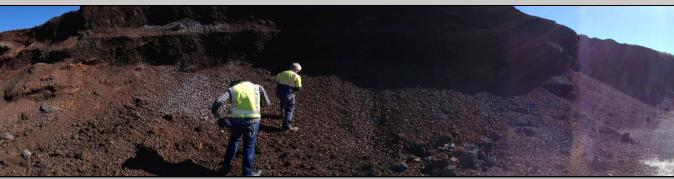
\includegraphics[scale=0.8]{figures/pile.jpg}
\caption{One of the stockpiles at the site.}
\end{figure}
    \chapter{Theory and Literature Review}
Modelling for the storage of BOS filter cake within stockpiles does not exist within the literature. The material is specific to the industry and presents its own challenges. In order to build appropriate models we utilise work conducted in existing industrial applications. We need to combine these models with the experimental data in order to provide useful models for stockpile ignition.

\section{Experimental work}
Experimental work has been conducted by Longbottom et al. \cite{Ray19} to evaluate the effectiveness of the filter cake to improve its recyclability. Through understanding the experimental work, we can use models to simulate the results and use the experimental data to fit these models. These experimental models can be used to develop more effective predictions in the larger stockpiles that we are interested in.

\subsection{Characterisation of the Material}
A key aspect of this thesis is the material used to build these stockpiles. The results from Longbottom et al. \cite{Ray19} determined the composition of the filter cake as well as the composition after some reactions had taken place. The important aspects of composition for this thesis, is the mass percentage of metallic iron and W\"{u}stite, 16.9\% and 29.8\% respectively. 
\subsection{Experimental Procedures}
One of the facets about this research project is the availability of experimental data. This allows more complicated models to be developed, as more parameters can be determined from experimental data. An additional benefit is that the models can be tested on smaller scales, to assess the accuracy. The relevant experimental techniques need to be understood in order to be able to model what is occurring.
%for more complicated models to be developed, as relevant data can be measured, though this requires a more thorough understanding of the experimental techniques and the relevant theory. 

\subsubsection{Thermogravemetric Analysis}
Thermogravemetric analysis (TGA), measures the weight change of a sample. A small sample is heated, usually at a fixed rate, and any deviation in mass is recorded. The technique is useful for assessing reactions such as oxidation and vaporisation, which have been observed from the experimental data for the filter cake \cite{Ray19}. Reactions such as melting and crystallisation cannot be investigated as the mass of the sample does not change \cite{thermal}.\\

In a small scale TGA experiment a 100 mg sample is placed in a crucible that is attached to a balance. Air is fed through the base of the set-up, and the sample is heated at a fixed rate via radiative heating. As the sample undergoes reactions the weight change is measured.\\

This set-up can be changed to include larger sample sizes, though this affects the quality of the data. With larger samples, significant temperature gradients within the sample can occur; as a result, diffusion needs to be considered and heating at a fixed rate becomes more difficult. Since the sample is larger, it can be representative of the stockpiled material. Having a bigger sample also improves the repeatability of the experiment.\\
\begin{figure}[h!]
\centering
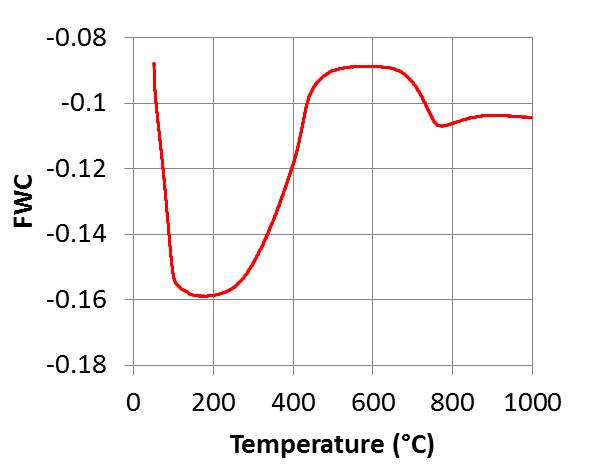
\includegraphics[scale=1]{figures/TGA_exp.jpg}
\caption{The Fractional weight change curve obtained from the TGA experiment \cite{Ray19}.}
\label{TGA_exp}
\end{figure} 
\subsubsection{Differential Scanning Calorimetry}
The set-up of the differential scanning calorimetry (DSC) is similar to that of the TGA. The experimental procedure of heating the sample is the same and as a result the two experiments can be conducted simultaneously. DSC however measures the heat of the reactions occurring in the sample. This is done by measuring temperature differences\cite{thermal}.\\  
\begin{figure}
\centering
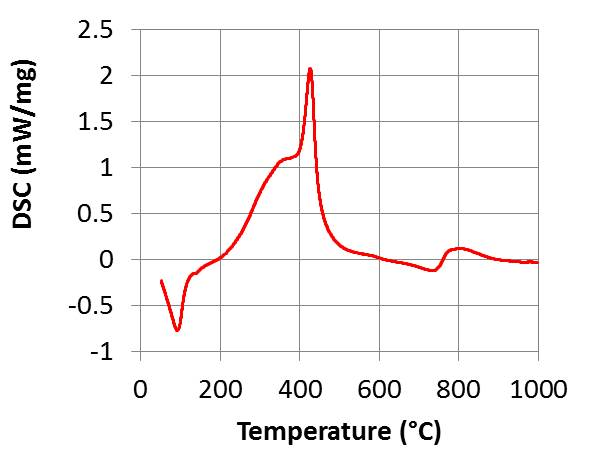
\includegraphics[scale=1]{figures/DSC_exp.jpg}
\caption{The DSC curve obtained through experimentation \cite{Ray19}.}
\label{DSC_exp}
\end{figure} 

\section{Frank Kamentskii Theory}
The fundamental theory of spontaneous combustion, is known as Frank-Kamentskii theory \cite{bowes}. The theory is based around temperature diffusion with an Arrhenius reaction term. The equation is,
\begin{equation}
\rho c\frac{\partial T}{\partial t}=k\frac{\partial^2 T}{\partial x^2}+Q\rho A\exp\left(\frac{-E}{RT}\right). \label{Comb_model}
\end{equation}
It is useful to consider the steady state solution of this equation.  
%include the scaled variables as well.
After rescaling the variables the steady state solution solves the differential equation,
\begin{equation}
\frac{d^2u}{dz^2}=-\delta\exp\left(\frac{u}{1+\varepsilon u}\right). \label{FK_mod}
\end{equation}
Using the Frank-Kamentskii approximation $\eps=0$, an analytic solution to the equation can be derived. This equation is the 1-dimensional analogue of Semenov's condition for ignition in a self-heating system \cite{bowes}.  The existence of this solution is dependant on the value for $\delta$ with two solutions existing for $\delta<\delta_{cr}$ \cite{bowes}. A large amount of combustion modelling uses this critical condition as a means of developing an ignition criteria for the stockpiles.
\subsection{Application to stockpile Ignition}
The model described in equation \eqref{Comb_model} has been used in a range of industries including oxidative heating, in materials such as coal and biological heating that occurs during composting \cite{bowes}. In each of these applications there are slight differences in how the theory is applied. 
\subsubsection{Compost}
In the composting process the method of heating cannot simply be taken as an Arrhenious reaction. Instead a second heating function is required to model the microbial heating.  Nelson et al.\cite{NELS03} proposed the following model,
\begin{multline}
\rho c_vV\frac{dT}{dt}=Q_bVF_b\frac{A_1\exp[-E_1/RT]}{1+A_2\exp[-E_2/RT]}B\left(1-\frac{B}{B_{max}}\right)+Q_cVA_3\exp\left[\frac{-E_3}{RT}\right]C\\-\chi S\left(T-T_a\right). \label{Bio}
\end{multline}
This has been used as a basis for much of the following work involving compost models. This model has been extended to a two-dimensional model with temperature diffusion \cite{sidhu06}. This latter model can be used to determine a critical ignition length for a stockpile.\\
An extension of this model is to introduce oxygen into the spatially uniform models \cite{nels07}.
The consumption of oxygen limits the reaction, and consequently the temperature. This base model has been extended into two dimensions with diffusion of oxygen \cite{Sidhu2007}.\\
When extending to multiple dimensions, an airflow is also added into the equations.
In the one dimensional case, airflow can only be considered in one direction \cite{luang09,luang10}. When in two dimensions, an equation is required to express the airflow through the stockpile. This is done as a forced flow where the airflow is independant of temperature \cite{luang10b,luang10c}. Aganetti et al. \cite{aga16} used a Darcy-Brinkman equation for flow in a porous medium. The airflow inside these stockpiles have been studied further with different flows able to be described. \cite{AGA17}\\
The  effect of moisture on the reaction has also been added into the model \cite{ZAM11,luang18,luang11a}. When modelling the moisture content, both a liquid water concentration and a water vapour concentration are needed. The concentration of liquid water affects the reaction rate; at higher water levels, there is an increased coverage of the reaction sites. The effects of ambient humidity, on the ignition criteria has been investigated \cite{luang18u} \\
Further additions to the model have been to consider different geometries \cite{luang11a} and also to use radiative boundary conditions \cite{luang10d,MOR09}. These developments add more complexities into the model but improves its accuracy.\\
%\subsubsection{Coal}
Many of the developments to these models can be adapted and applied to filter cake stockpiles. There are some key points where the two problems differentiate, one of which is the construction of the stockpiles. The stockpiles are built up gradually over time and this has to be taken into account. The compost models focus on preventing combustion, so when the stockpile is increased in size, a cautious approach would be to consider fresh compost. This will underestimate the critical combustion length. The need for a model that considers a changing domain is dependant on the consumption of reactants due to this.

\subsubsection{Coal}
Coal stockpiles have also been modelled using the FK framework \cite{Zhang16}. 
\subsubsection{Periodic Boundary conditions}
The basic model can be adapted by change the boundary condition. One such method is to have an oscillating ambient temperature. The stockpiles are exposed to diurnal and seasonal temperature variation. Shteinberg and Khudyaev \cite{shtein05} proposed an ODE model, given by,
\begin{align}
\frac{d\theta}{d\tau}&=a\E^\theta-\frac{1}{\delta}\left[\theta-\theta_A\sin\left(\frac{\omega\tau}{\delta}\right)\right],\\
\frac{da}{d\tau}&=-\gamma a\E^\theta,
\end{align}
for the averaged temperature and reactant consumption across the domain. Gorel'skii et al. \cite{gorel10}, analysed this model. These models do not consider the diffusion of temperature, so cannot distinguish regions that have different temperatures. \\
Novozhilov \cite{novozhilov16} proposed a model in one dimension with a single sinusoidal, oscillating boundary. Critical dependencies for the non-dimensionalised amplitude of the oscillations, were developed in terms of the other variables. The analysis was limited to the scaled equations rather than providing any direct application to any problems. Both convective heat transfer and fixed temperature boundary conditions were considered.\\
Novozhilov \cite{novozhilov18} added reactant consumption to the model, using a first order reaction scheme. The effects of having an initial condition that differs from the ambient temperature is also added \cite{novozhilov18}. As more complexities are introduced into the model there are more parameters to investigate. The study similarly determined critical dependencies of the scaled amplitude oscillations. Providing a critical condition for this scaled oscillation amplitude, does provide some insight into the problem, however, it does not address ways to prevent or promote ignition. This parameter does not include variables such as the stockpile length which can be controlled.\\ 
Roy \cite{roy18} proposed a two dimensional model to investigate the effects of oscillating boundary conditions. The proposed model included an oscillating boundary condition along one of it's edges with fixed temperatures on the other edges. It included convection terms, though limited this to a closed system (no air flowing in or out of the domain). As such, the model is more applicable to an experimental set-up, rather than to assess the ignition in large stockpiles where the oscillations are expected on the majority of the boundary.\\ 
We see that there is comparatively limited work with oscillating boundary conditions. The current models proposed are limited in their dimensions and subsequently their application to large stockpiles. The models are restricted to one sinusoidal function, whereas a model including both seasonal and diurnal temperature variation may be more appropriate.
%cite reference for dual sinusoidal weather function.
 It may also be useful to use include the weather data that has been recorded, as this will be more accurate than using a sinusoidal function.

\subsection{Theory applied to experimental work}
\label{Kis}
The models used for thermogravemertic analysis have been reported in studies from Flynn and Wall \cite{flynn66} and Sharp \cite{sharp69}. In these studies the proposed model was in terms of conversion, given,
\begin{equation}
\frac{dC}{dt}=kf(C), \label{fl}
\end{equation}
where k is reaction dependant. In this case the conversion, C, can be expressed as, $C=1-\left(\left(W-W_f\right)/\left(W_0-W_f\right)\right)$, where $W$ is the weight, $W_f$ is the final weight, and $W_0$ is the initial weight. This implies that the initial concentration, $C(0)=0$ The expression for $f(C)$, is dependant on the reaction order. For a reaction of order $n$,
\begin{equation}
f(C)=(1-C)^n.
\end{equation}
This has the effect that for higher concentrations the reaction is accelerated and slows once more of the reactant is consumed. The reaction rate $k$, varies with temperature per an Arrhenious expression, \\
\begin{equation}
k=A\exp\left(\frac{-E}{RT}\right),
\end{equation}
where, A is a pre-exponential rate factor, E is the activation energy, and R is the ideal gas constant.\\
It is not necessary to write the equations in terms of the conversion factor. Ozawa \cite{ozawa65}, uses the weight directly. The equation is,
\begin{equation}
-\frac{dW}{dt}=A\exp\left(\frac{-E}{RT}\right) W^n. \label{oz}
\end{equation} 
It is straightforward to show that these equations are equivalent. This requires equation \eqref{oz}, to be rescaled by the initial weight. In the two equations, the interpretation of the pre-exponential factor is different. This can be seen from dimensional analysis. For equation \eqref{oz}, $\frac{dW}{dt}$ has units $MT^{-1}$, where $M$ is units of mass and $T$ is units of time. As a result $A\exp(E/RT)W^n$ must also have units $MT^{-1}$. The exponential term is dimensionless, and $W^n$ has dimension $M^n$. As a result the dimension of the pre-exponential factor is $M^{1-n}T^{-1}$. For equation \eqref{fl}, there is no mass dimension involved in the equation as we are dealing with the dimensionless conversion factor $C$. The only units involved are time and since the reaction rate $k$ must have units $T^{-1}$, the pre-exponential factor, $A$, must have dimension $T^{-1}$. The units are only the same when the equation is first order, $n=1$. In this case the reaction is invariant under scaling of $W$. It is also useful to note that different reaction order equations have different pre-exponential factors.
The same equations have been used in other studies to evaluate the kinetic parameters A and E \cite{carrasco93,kissinger56,sbirrazzuoli97}.\\
Kissinger \cite{kissinger56} developed a method that can be used to determine the reaction constants, $A$ and $E$. This method was to examine when the reaction rate is at its peak. The reaction rate for Equation \eqref{oz} is at it's maximum when, 
\begin{equation}
\frac{d}{dt}\left(\frac{dW}{dt}\right)=0.
\end{equation}
In the work carried out by Kissinger, it was assumed that the reaction order was one. This resulted in the equation,
\begin{equation}
A\exp\left(\frac{-E}{RT_m}\right)=\frac{E}{RT_m^2}\frac{dT}{dt},
\end{equation}
where $T_m$ is the temperature at which the maximum reaction rate occurs, and $\frac{dT}{dt}=\alpha$, which is the heating rate in the experiment. By taking logarithms straight line equation can be formed, for the variables, $X=1/T_m$ and $Y=\log\left(\alpha/T_M^2\right)$ allowing a linear regression to be performed. If we do not assume the reaction order, then an additional term, the amount of converted material, is required. From this equation the reaction order and the kinetic parameters can be estimated. To estimate the parameters in this way, we must be able to determine the Temperature at which the maximum reaction rate is achieved. With two reactions this is difficult to achieve. This equation is still useful in being able to relate our parameters.\\
%As an aside, for this reaction problem where we have two distinct reactions occurring, determining the converted fraction of material will be difficult. As a result the simplifying assumption is to take a first order reaction.
\subsection{Critical Ignition Criteria}
The Frank-Kamanetskii theory states that for the case when $\delta<\dcr$, there exists a low temperature solution and a high temperature solution \cite{Gray93,bowes}. Various ignition criteria have been investigated. Weber et al \cite{weber98} investigates the effects that different families of initial conditions have. These include, constant, linear and quadratic initial temperature profiles. These initial investigations provided some useful critical ignition conditions though they lack any consumption of material. Brindley, Griffiths and McInstosh \cite{brindley01} address this by introducing consumption and also restricting their analysis to an embedded hotspot. They numerically examinded some criteria required to iniate combustion waves. The existence and propogation of combustion waves have been well studied by various authors \cite{merzhanov88,gubernov12,mcintosh04,weber97,mercer96}. 
McIntosh, Brindley and Griffiths \cite{mcintosh02} futher build upon their work to produce an analytic approach to this problem. This extends previous work that has been done on strongly reactive material \cite{Jackson89,kapila81}. The hotspots examined used a constant power source for their hotspot. For our industrial stockpiles we use a hotspot consisting of previously reacted material.\\

More recent work from Shah et al \cite{shah07} examines hotspots more consistent with the tyoe we are interested in. This research examines the smoldering bahaviour where the reaction rate is controlled by a low oxygen concentration where the reactions are occurring. The key introduction here is the introduction of Oxygen into the model and the subsequent porosity. This theory has been applied to numerical and experimental studies into ignition by a heated particle \cite{wang15,glushkov11}. Similar experimental work has been done by Caine et al \cite{caine10} where they investigated a hotspot with constant power.\\

These studies have developed a lot of theory regarding the ignition of materials using hotspots. One area that appears to be lacking, is the use of previously reacted material. 


\subsection{Parallel Reactions}
Much of the standard approach to Frank-Kamanteskii theory uses a single reaction. The work of Longbottom et al. \cite{Ray19} indicates that we may have several reactions occuring during the sintering process. Boddington et al. \cite{bodd84} developed the foundations of Frank-Kamenetskii theory with parallel reactions. The paper determines a method to calculate an effective activation energy and FK parameter. This then reduces the parallel reactions to a single reaction for which we can apply the existing theory for. Graham-Eagle and Wake \cite{GE85} extended this theory to determine the critical FK parameter in an infinite cylinder and sphere. Graham-Eagle and Wake \cite{GE86} then extend this further to examine the effects of introducing an endothermic reaction. All previous work had only considered exothermic reactions as these are the drivers of self-ignition. This theory has been used to simplify reaction equations in various different contexts and with differing numbers of reactions \cite{wake92,push89,ajadi09,jones91}. \\

Wake et al. \cite{wake92} used this theory to examine heating in forest litter and coal. Pushpavanam and Narayanan \cite{push89} considered the effects of having an endothermic and exothermic reaction in parallel to investigate the ignition and extinction points of the steady state solution. Ajadi and Gol'dshtein \cite{ajadi09} studies the critical behaviour of a three step reaction scheme using this technique.  
 

\subsection{Moisture}
Moisture can be an important factor to consider. There have been instances in the literature \cite{back81,walker67,lohrer05} where wetting of dry material has been found to have caused ignition. Gray and Wake \cite{gray90} models this ignition phenomenon by using a series of parallel reactions. They considered the heat generated through the wetting process and also the cooling effect of evaporation. These two concepts are important to address in investigating our stockpiles. 

\subsubsection{Drying}
Different drying models have been proposed \cite{chen98}. This includes a reaction engineering approach that models evaporation as an Arrhenious expression with activation energy as the latent heat of vaporisation. Similarly condensation is modelled using a zero activation energy assumption. This form of drying was used by Luangwilai \cite{luang11} when investigating how moisture is evaporated in the compost piles.\\
Chen \cite{chen98} proposed a model that looks at evaporation and condensation in terms of an exchange between two surfaces. The change in concentration is proportional to the difference in concentration at the inner surface, and the surface area. Similarly we have a change occurring that is proportional to the concentration difference on the outer surface. The advantage of this approach, is that it considers the concentration of water vapour within the sample, to be distinct from its concentration in ambient air. The issue with this model is that it introduces additional parameters. One of the new terms introduced is the surface area of the small scale particles within the sample. In the context of our material, that does not appear to be a feasible option, as determining the surface area is quite complicated. For simplicity, we therefore use the reaction engineering approach to drying.

\subsubsection{Affect on the reaction}
Characterising how the moisture affects the reaction is not a simple task. We can consider inhibition due to covering the surface available for the reaction. Luangwilai \cite{luang11} used this approach when modelling the combustion of organic material in compost heaps. It was assumed that if the concentration is above a critical concentration, then the reaction would stop. The function is normalised so that when there is no water then the reaction is maximised and the effect of moisture is set to 1. Then the function decreases to 0 as the water concentration approaches some critical concentration. \\
More work needs to be done experimentally to characterise how the moisture levels affect the reaction. From the TGA data provided by Longbottom et al.\cite{Ray19}, it appears as though the reactions are activated at temperatures above the evaporation point of water. This may indicate that the water woould not have any effect as the reactions are not significant at those low temperatures.



\subsection{Radiation effects on Conduction}
The effect of radiation on stockpile ignition is not a common consideration. The modelled stockpiles usually are to prevent ignition \cite{Zhang16}. Mercer and Weber \cite{mercer97} studied the effects of radiative transfer on combustion wave speeds. The radiation effects included was in terms of a radiative heat flux. The net radiative energy emitted and absorbed by the matter per unit time per unit volume is given by $ \nabla \cdot \mathbf{q}^r$, where $\mathbf{q}^r$ is the radiative heat flux  \cite{ozisik73}. The Eddington approximation in one direction is given by the differential equation,
\begin{equation}
\frac{d^2 q^r(\tau)}{d\tau^2}=(1-\omega)\left[4\pi\frac{dI_b(\tau)}{d\tau}+3q^r(\tau)\right],
\end{equation}
where $\omega$ is the albedo, and $I_b(\tau)$ is the total black-body radiation intensity. We can relate the total black-body radiation intensity to the Temperature, 
\begin{equation}
I_b(x)=\frac{\sigma n^2 T(x)^4}{\pi}, \label{black_body}
\end{equation}
where $\sigma$ is the Stefan-Boltzman constant and $n$ is the refractive index. This approximation is for optically thick medium, as a result, this approximation is not as accurate near the boundaries \cite{ozisik73}. In the literature \cite{joulin86,mercer97} the approximation has been altered to,
\begin{equation}
L^2\frac{d^2 q^r(x)}{dx^2}=\left[4\pi L\frac{dI_b(x)}{dx}+3q^r(x)\right],
\end{equation}   
where L is the local absorption length. When the local absorption length is small compared to the length of the medium, then a simplified expression can be used,
\begin{equation}
q^r(x)=-\frac{4\pi}{3} L\frac{dI_b(x)}{dx}.	\label{qr}
\end{equation}
This is the case of optically thick mediums \cite{mercer97}.\\

When incorporating this into the model given by equation \ref{Comb_model} we have, 
\begin{equation}
\rho c\frac{\partial T}{\partial t}=k\frac{\partial^2 T}{\partial x^2}+Q(T)+\frac{\partial q^r}{\partial x}. \label{Rad_model}
\end{equation}
This was investigated by Mercer and Weber \cite{mercer97}. Substituting in equations \ref{black_body} and \ref{qr} and rearranging we obtain,
\begin{equation}
\rho c\frac{\partial T}{\partial t}=\frac{\partial}{\partial x}\left(\left(k-\frac{16}{3} L \sigma n^2 T^3\right)\frac{\partial T}{\partial x}\right) +Q(T).
\end{equation}
This equation provides an effective radiative conductivity, $k_r$ that satisfies $$q^r(x)=-k_r \frac{dT}{dx}$$.

%\section{Ignition of metal powders}

\section{Parameter Estimation}
An important aspect of our modelling is determining the parameter values for the reaction model. Experimental work has been conducted on the BOS filter cake \cite{Ray19,ray20}. We use the TGA and DSC data to fit our model. One of the common approaches is to use that of Kissinger \cite{kissinger56} outlined in section \ref{Kis}. This uses the equation,
\begin{equation}
A\exp\left(\frac{-E}{RT_m}\right)=\frac{E}{RT_m^2}\frac{dT}{dt}, \label{eqkis}
\end{equation}
with different heating rates and corresponding maximum temperatures. Taking logarithms we can rearrange equation \ref{eqkis} to,
\begin{equation}
\log\left(\frac{\alpha}{T_m^2}\right)=\log\left(\frac{AE}{R}\right)-\frac{E}{R}\frac{1}{T_m}.
\end{equation}
This is a straight line for the variables, $X=1/T_m$ and $Y=\log\left(\alpha/{T_m^2}\right)$, allowing a linear regression analysis. This method is not as useful for systems where multiple reactions are occurring. The reason for this is that we cannot determine the temperature at which the reaction rate for each reaction is maximised.\\
Another approach is to use the critical FK parameter, $\delta$. The FK parameter is given by,
\begin{equation}
\delta=\left(\frac{L}{2}\right)^2\frac{QCA}{k}\exp\left(\frac{-E}{RT_a}\right)\frac{E}{RT_a^2}.
\end{equation} 
Taking logarithms we can rearrange this to,
\begin{equation}
\log\left(\frac{4 \delta T_a^2}{L^2}\right)=\log\left(\frac{QCA}{k} \frac{E}{R}\right)-\frac{E}{R}\frac{1}{T_a}. 
\end{equation}
The hot storage test heats a basket of material at a fixed ambient condition. By determining which ambient temperature causes the basket to ignite, for multiple size baskets, we can use a regression model to determine the parameters \cite{gray84}. Jones and Wake \cite{jones90} used this method to determine the kinetic parameters for several materials. This method also has similar issues as it only considers one reaction. Jones \cite{jones92} uses the work of Boddington et al. \cite{bodd84} on parallel reactions to modify this method for two reactions. This adjustment relies on knowing some information that we do not possess. However in our stockpiles the exact reactions have not been determined so those know parameters are not known in our stockpiles.\\

Include two other techniques here mentioned by zanoni.\\

These standard techniques are insufficient to estimate the kinetic parameters when we have multiple reactions. We cannot know what the temperature is which maximises each reaction rate. Another approach is to use an optimisation algorithm. Elliot et al. \cite{elliot05} use a genetic algorithm as an optimasation tool for a system of parallel reactions.  Zanoni et al. \cite{zanoni12} used a Levenberg-Marquardt algorithm to determine the kinetic parameters in a reaction scheme. The objective functions in these cases are complex, exhibiting multiple local minima and maxima, as such gradient based optimisation algorithms are not as successful \cite{elliott05}. Reverte et al. \cite{reverte07} also used a Levenberg-Maraquardt algorithm. They used this to determine an optimal experimental design in order to minimise the error in the parameters estimated. They optimised the design for sample weight, temperature profile, and gas flow rate. The objective fuction minimised was a sum of squares of the measured data and the predicted data.\\
Using these techniques, quantifying the uncertainty in the model becomes more difficult. We use a Markov-Chain Monte-Carlo (MCMC) method to estimate our parameters. An outline of the method is provided in the Appendix. The main advantage of using a MCMC algorithm, is that we are able to draw a sample from the distribution of possible parameter values. We can use this sample to estimate posterior expectations for different quantities including the critical length of the stockpiles. The optimisation based methods allow the variance around the optimum value to be determined, but does not naturally allow a sample to be obtained and parameters to be transformed.\\
The Bayesian approach has been used in recent studies of coal blends \cite{buyu17,buyu17p}. These studies used Monte-Carlo simulations in order to characterise the uncertainty in the predictor coefficients for a multiple non-linear regression analysis. This is a similar idea to our approach, however we assess the uncertainty of parameters in an ODE model.\\


    \chapter{Model Definition}
In this chapter we define each of the models that we use as well as some of the variations. Having a clear model is the first stage in being able to predict future behaviour. We begin by ptoviding the base model that we use to form the basis of our stockpile models. We then present some of the variations to the model that can be made. We do not investigate these changes until Chapter \ref{results}. After presenting the models for the stockpile we look at the models we use for modelling the TGA experiment.

\section{Stockpile Model}
\label{Sec:stockpile}
The first model we examine is for the large stockpiles. To model such stockpiles we use the Frank-Kamenetskii (FK-theory). We consider the equation,
\begin{equation}
\rho c \frac{\partial T}{\partial t}=\nabla \cdot \left(k\nabla T\right) +Q(T), \label{base}
\end{equation}   
where the parameters are defined in the nomenclature, and $Q(T)$ represents heat generation inside the stockpiles. Equation \ref{base} provides the basis for which we build our models. Inside the stockpiles we have multiple reactions occurring. Longbottem et al. \cite{Ray19} conducted experimental work on the material found inside the stockpiles. Multiple reaction schemes have been proposed by Longbottom et al \cite{Ray19}. We consider a sequence of two parallel reactions,
\begin{align*}
3\text{Fe}+2\text{O}_2 &\rightarrow \text{Fe}_3\text{O}_4, \\
6\text{FeO}+\text{O}_2 &\rightarrow 2\text{Fe}_3\text{O}_4. \\
\end{align*} 
We can model these reactions through an Arrhenius reaction rate. The reaction rate is given by,
\begin{equation}
k(T)=A\exp\left(\frac{-E}{RT}\right). \label{arrhenius}
\end{equation} 
Using the Arrhenius reaction rate, Equation \ref{arrhenius}, for two reactions, Equation \ref{base} becomes,
\begin{equation}
\rho c \frac{\partial T}{\partial t}=\nabla \cdot \left(k\nabla T\right) +Q_1A_1\exp\left(\frac{-E_1}{RT}\right)+Q_2A_2\exp\left(\frac{-E_2}{RT}\right). \label{FK_eq}
\end{equation}
The parameter $Q$ is to the heat generated from the reaction. Equation \ref{FK_eq}, is a heat balance equation that describes the rate at which energy inside the stockpile changes. This formulation is valid for any geometry.\\
One key consideration in proposing a model is understanding the assumptions that are placed on the model. The assumptions simplify the model but we cannot make too many assumptions otherwise the information gained from the model is not useful. We have made the following assumptions:
\begin{itemize}
\item The filter cake is a homogeneous material.
\item No material is consumed by the reactions.
\item Heat is only transported via conduction.
\item Oxygen is not depleted within the stockpile. 
\item The change in filter cake density is negligible.
\end{itemize}
These assumptions are necessary to simplify the problem into something that we can investigate. The filter cake is naturally a heterogeneous material. We are unable to quantify this heterogeneity and as such cannot factor this into the model. %Another factor that makes this complicated is measuring the effects that the material has on each parameter. Because of this then we can use effective parameters that assume the material is homogeneous and these will be the parameters obtained through experimentation.
\\
Within the stockpiles oxygen, iron and  w\"{u}stite are all consumed as part of the reactions. In the combustion literature it is standard to assume that the material is not consumed \cite{Zhang16}. The argument is that most models are interested in preventing ignition and the material depleted before ignition is often not significant. Oxygen is often added into models after the initial investigations. We eventually remove this assumption.\\
For outdoor stockpiles there are other mechanisms of heat transfer. Wind can transfer energy within the stockpile. Radiation is another form of energy transfer that is usually not considered. Advection is typically added into a model using simple models. These do not account for the variation in wind that occurs naturally. %cite. 
Radiation as a form of energy transfer is not usually considered as the effects are often small at low temperatures.\\
Through the course of this thesis we aim to remove some of these assumptions in order to develop the model to provide more realistic predictions.\\
\subsubsection{Oxygen}
We add a mass balance equation for oxygen into the model. One factor to consider is the consumption of oxygen by the reaction. We modify the reaction rate equation \ref{arrhenius}, to include oxygen as a factor. We assume a first order reaction for simplicity, though this may prove to be insufficient. The modified equation becomes.
\begin{equation}
k(T)=OA\exp\left(\frac{-E}{RT}\right). \label{Arr_Oxygen}
\end{equation}
This now includes oxygen as a controlling factor in the reaction rate. If the oxygen concentration is zero, then the reaction ceases. Using equation \ref{Arr_Oxygen}, the mass balance equation is,
\begin{equation}
\frac{\partial O}{\partial t}=D\nabla \cdot \nabla O - OA\exp\left(\frac{-E}{RT}\right). \label{O2_equation}
\end{equation}
This model is limited to include the diffusion of oxygen and does not include advection. Adding Equation \ref{O2_equation} into the model removes the previous assumption we made that oxygen is not depleted within the stockpile. We still make assumptions about how oxygen moves throughout the stockpile and we also have to make assumptions as to how oxygen is exchanged at the boundary. These assumptions are more realistic than oxygen not being depleted and as such this addition is made to the model.

\subsubsection{Material Consumption}
Consumption of the material within the stockpile is usually not considered in models for spontaneous combustion. In many applications of combustion theory \cite{Zhang16, NELS03,RESTUCCIA17}, the objective is to identitify the conditions for self-ignition in order to prevent a loss of material. In these cases if the material has undergone a significant depletion then the objective has failed. The result is that this assumption is acceptable in these cases. Ignoring the depletion of material is a worst case scenario approach. Any conditions that are imposed on these models to limit self-heating will apply to the stockpiles with reactant depletion.\\
The stockpiles that we are interested in are used to recycle the filter cake. In this case it is desirable for the stockpiles to undergo self heating. It may also be useful to be able to model the stockpiles at high temperatures in order to predict where the material has sintered. In order to make the model useful at high temperatures we need to consider the consumption of reactants.\\
To include material consumption into our model we consider the effect it has on the reaction rate. We consider a first order arrhenius reaction for simplicity. Equation \ref{Arr_Oxygen} becomes,
\begin{equation}
k(T)=MOA\exp\left(\frac{-E}{RT}\right), \label{Arr_Mat}
\end{equation}
where $M$ is the mass density of the reactant. When introducing the reactants into the model we have to make some consideration for the units. We go into detail about determining units in section \ref{SEC:TGA}.\\
The material within the stockpile is a solid, as such we do not consider any transport within the stockpile. Similarly to when we introduced oxygen an assumption is removed, no depletion of reactant. New assumptions are made about how material is moved through the stockpile and the effect it has on the reaction. These assumptions are more reasonable than the material having no reactants consumed in the reaction.\\

\subsection{Boundary Conditions}
\label{Sec:models:BC}
A partial differential equation (PDE) model requires boundary conditions. The boundary conditions can be adjusted in order to add more complexities into the model. The most basic boundary condition is the Dirichlet condition,
\begin{equation}
T=Ta. \label{base_BC}
\end{equation}   
It is often assumed that the ambient temperature is constant. This assumption does not have to be made and we remove this by investigating the effects of periodic boundary conditions. The Dirichlet boundary condition assumes that there is perfect heat transfer between the external boundary and the air. This can be overcome by introducing Newtonian cooling boundary conditions,
\begin{equation}
\frac{\partial T}{\partial n}=-h\left(T-T_a\right), \label{Newton_cooling}
\end{equation}
where $\frac{\partial T}{\partial n}$ is the outward unit normal derivative. Similarly to the dirichlet condition, the ambient temperature is usually considered fixed. For the newtonian cooling condition we have the limiting case, as $h\rightarrow \inf$, then the boundary condition approaches the Dirichlet condition, $T=T_a$. This condition indicates perfect heat tansfer between the boundary and ambient air.

\section{Thermogravimetric Analysis Model}
\label{SEC:TGA}
As part of this thesis we require a model that simulates the TGA experiment. This model is used to estimate the reaction parameters used in Equation \ref{arrhenius}. The TGA experiment provides some data that can be used whereas the stockpiles alone cannot provide these estimates. We will build this model using Equation \ref{Arr_Mat}. Equation \ref{Arr_Mat} is the rate at which the reaction is occurring. By carefully selecting the appropriate units, we can express this as the rate at which a mass, $M$ is consumed by the reaction. We also want to consider our choice of units in the context of the stockpiles. We do this to ensure consistency to allow for the reaction parameters to be used easily in the stockpile models. We model the TGA experiment by the system of equations,
\begin{align}
\frac{dM}{dt}&=-MOA\exp\left(\frac{-E}{RT}\right), \label{TGA_system} \\
\frac{dT}{dt}&=\alpha. \label{TGA_system2}
\end{align}
This system represents the mass lost through a reaction as the temperature is increased at a constant rate. To use the system of equations \ref{TGA_system}, we make the following assumptions:
\begin{itemize}
\item The temperature is constant throughout the sample and is increased at a fixed rate.
\item Oxygen levels are constant for the duration of the experiment.
\end{itemize}
These assumptions are reasonable based on the experimental design. The constant temperature is justified due to the small size of the sample. The sample is 100 mg and the temperature diffusion within the sample is negligible. The experiment has a continuous inflow of air. We assume this inflow replaces oxygen consumed during the reaction. If we removed any assumptions then it adds more complexity into the model. We could measure the oxygen concentration at the outflow point in order to determine the validity of this assumption.\\
We still need to determine an appropriate set of units. From dimensional analysis we have,
\begin{equation}
\frac{\left[M\right]}{\left[t\right]}=\left[M\right]\left[OA\right].
\end{equation}
Since $\left[M\right]$ appears on both sides of the equation then its units does not matter for the TGA experiment. For the TGA model we use mass for the units of $M$. We choose to use mass since it is easy to convert the equation into a mass density equation for models that consider spatial dimensions. Since we can scale $M$ by a constant then if we assume that the volume is kept constant and the mass doesn't change spatially then the equation remains true. When mass does change spatially then the change in mass density follows the mass change equation in equation \ref{TGA_system}.\\
We now consider appropriate units for oxygen. In the context of the TGA experiment it does not matter as oxygen is kept constant. In the large stockpiles the concentration is the most natural quantity to consider. When we include consumption of iron, our reaction rate is expressed as the rate at which a mass of iron is consumed. In order to determine how much oxygen is consumed at the same time it is easiest to work in terms of a mass of oxygen rather than a concentration. We are still able to convert mass density into a concentration and this is done after the simulation is complete. The pre-exponential factor, $A$, subsequently has units, $[A]=\text{m}^3/\text{kg}/\text{s}$. We may scale this constant to have different units of time depending upon the context.\\
In order to model the TGA experiment conducted by Longbottom et al. \cite{Ray19}, we consider a two reaction system. We only consider simulating the region that is considered from $130-600^oC$. This is where the bulk of the self heating is expected to occur in the large stockpiles. Prior to this region, moisture is being removed from the sample. There is a possibility that more reactions occurr in this region; we expect two reactions are sufficient to simulate the experiment. The TGA experiment measures the total mass of the sample. Our model equations are for the mass of the individual components being consumed. This means that we need an equation for the sample mass.
The sample mass is given by,
\begin{equation}
\frac{dM_t}{dt}=w_{c,1}M_1A_1\exp\left(\frac{-E_1}{RT}\right)+w_{c,2}M_2A_2\exp\left(\frac{-E_2}{RT}\right), \label{FWC_equation}
\end{equation}
Where the subscripts 1,2 refers to the first and second reaction respectively, $M_1,M_2$ follow the system given by equation \ref{TGA_system}, and $w_c$ refers to the change in sample mass per $M$ consumed.\\
This now forms a complete system that can be used to simulate the TGA experiment. In the next chapter we use the TGA experiment to estimate the parameters in our model in order to translate this into the larger stockpiles. 

\subsubsection{Differential Scanning Calorimetry}
During the TGA experiment, Differential Scanning Calorimetry (DSC) can be conducted. This provides additional data that we can use to estimate the kinetic parameters. In order to do this we need to simulate the DSC data. We can do this using the equation,
\begin{equation}
H=Q_1 \frac{dM_1}{dt}+Q_2 \frac{dM_2}{dt}. \label{eq:dsc}
\end{equation}
This equation introduces a heat of reaction parameter $Q$, for each reaction. This is the same parameter that is introduced in our stockpile. We can rewrite Equation \ref{eq:dsc} by substitung the arrhenous reaction rates. This form allows a simple calculation to be made once we have solved the system of equations.\\

We have established the various models that we conduct our analysis on. We have also stated the necessary assumptions that unperpin each of the models. These assumptions all simplify the model down. We conduct anaylsis on each of these models and present different alterations to these.
    \chapter{Bayesian Inference}
\label{Ch:Infer}
In this chapter we present Markov-Chain Monte Carlo (MCMC) algorithms to estimate the Bayesian posterior distribution of the parameters in our Thermogravemetric Analysis (TGA) model. We begin by investigating the effectiveness of this method on a simulated, single reaction TGA. We then apply this to a simulated experiment with two parallel reactions, before applying the algorithm to experimental data. At each stage we look for issues that arise with the algorithm and how to refine this for our application in thermogravemetric modelling. The test cases provides a framework with known parameters and conditions. The key advantage of the simulated data is that we know the underlying parameters and the model predicts exactly the behaviour of our system. For the experimental data we also face the potential issue of model misspesification \cite{KEN01,Bry14}\\

For each application we apply the same basic statistical model. Let, $F(\theta_M)$ denote the vector corresponding to the solution of the relevant ODE equation, evaluated at the times, $t$. The symbol, $\theta_M$ denotes
the parameters required for the differential equation. The simulated data, $y$ is generated by, adding Gaussian noise to the simulation. Our liklihood function is, 
\begin{equation}
\textbf{y}~ \sim ~N\left(\textbf{F}\left(\theta_{M}\right),\sigma^2\textbf{I}\right). \label{eqn:liklihood}
\end{equation}
To evaluate this liklihood we are required to solve the ODE equation. We solve the ODE numerically using a simple Runge-Kutta algorithm. The posterior distribution follows the equation,
\begin{equation}
P(\theta|\textbf{y})=\frac{P(\textbf{y}|\theta)P(\theta)}{\int P(\textbf{y}|\theta)P(\theta) d\theta},
\end{equation}
where, $\theta=\left(\theta_M,\sigma\right)$ represents our parameters, $P(\textbf{y}|\theta)$ follows the liklihood function in Equation \ref{eqn:liklihood}, and $P(\theta)$ is the prior for our parameters which generally a uniform distribution. $P(\textbf{y})=\int P(\textbf{y}|\theta)P(\theta) d\theta$ is a normalising constant, sometimes referred to as the model evidence. Since the likelihood \ref{eqn:liklihood} requires the solution to the ODE, $P(\textbf{y})$ is unavailable in closed form. Instead we use MCMC methods to simulate from the posterior $P\left(\theta|\textbf{y}\right)$.\\
\begin{algorithm}[H]
\SetAlgoLined
\KwResult{Write here the result }
 Initialise $\theta$ by sampling from the prior\;
 \While{sample_size $<$ required sample}{
  Sample $\theta ^*~ \sim ~ Q(theta^*|\theta)$ \;
  Set $\alpha = \frac{P(\textbf{y}|\theta^*)Q(\theta_{t-1}|\theta^*)P(\theta^*)}{P(\textbf{y}|\theta)Q(\theta^*|\theta_{t-1})P(\theta_{t-1})}$\;
  Sample $b ~ \sim ~U(0,1)$\;
  \eIf{$\alpha>b$}{
   Set $\theta_t=\theta^*$} {
   Set $\theta_t=\theta_{t-1}$
   }
 }
 \caption{Metropolis Hastings Algorithm}
 \label{Alg:MH}
\end{algorithm}
The MCMC algorithm we use is a Metropolis-Hastings Algorithm outline in Algorithm \ref{Alg:MH}. Our algorithm proposes new parameters, $\theta ^*$, using a Gaussian random walk proposal, centered on the previous parameters. This proposal has the advantage of being symmetric, $Q(\theta |\theta^*)=Q(\theta^*|\theta)$. This reduces the amount of computations that are required when determining the likelihood, $\alpha$ in Algorithm \ref{Alg:MH}.\\ 
We have not yet defined the variance of the Gaussian proposal distribution. When selecting this variance it is important to consider what acceptance rate is acceptable. If the acceptance rate is too large, then the algorithm may not have explored enough of the parameter space. A low acceptance rate increases the number of iterations required to generate our sample. There are numerous ways to consider the optimal acceptance rate. Roberts et al. \cite{Rob97} and Yang et al. \cite{Yang20}  indicates that an acceptance rate of 0.234 can be obtained under some conditions. Achieving a rate similar to this over the course of the algorithm is unlikely. At different stages of the algorithm we want different acceptance rates. In an ideal case, the early stages of the algorithm quickly locates the maximum likelihood point. To achieve this a large variance is considered. Once the algorithm is near this local maximum more precise steps are required to generate a sample from the posterior distribution. We vary the variance to allow greater steps to occur initially and smaller steps to occur later in the algorithm.\\
The initial values proposed in the algorithm are heavily dependant upon the starting point. At this stage, known as the transition phase, the algorithm has yet to converge and is not approximating the posterior distribution. These values are considered the burn in for the algorithm and must be discarded. Our algorithm is set up so that a fixed number of points are proposed. To discard the burn in points we take a fixed sample size from the end of the chains and discard all but the last 1000 values.\\
The algorithm is dependant upon the starting values. In our simulations we create four chains, each with different starting values. Each chain follows the same process outlined in Algorithm \ref{Alg:MH}. This is particularly important when the posterior distribution has multiple modes. This is also a key advantage of using the MCMC approach as traditional optimisation methods can become stuck in the suboptimal modes. %cite

\section{Single Reaction}
\label{Sec:1R}
To develop the MCMC algorithm, we need to define our model and model parameters. We use the model
\begin{align}
\frac{dM}{dt}&=-MOA\exp\left(\frac{-E}{RT}\right), \label{TGA_system_BI} \\
\frac{dT}{dt}&=\alpha, \label{TGA_system2_BI}
\end{align}
derived in section \ref{SEC:TGA}. In this application since the oxygen level does not change, then this constant is absorbed into the pre-exponential factor $A$.\\
Using this model, we consider the parameters $A$ and $E$. We also need a parameter $\sigma$ that represents the noise of our data. We set the true parameters to be $A_{\text{true}}=3.17\times10^6 \text{min}^{-1}$, $E_{\text{true}}=8.616\times 10^4 \text{J}/\text{mol}$, and $\sigma_{\text{true}}=0.05$. Since the parameters $A$ and $E$ can vary significantly on a log scale we explore the parameter space using the parameters, $\tilde{E}=\log_{10}E$ and $\tilde{A}=\log_{10}A$. This is a key transformation allowing the algorithm to explore many orders of magnitude much more easily than if we used the original variables. This can reduce the burn in time and provide greater precision. Our vector of parameters, $\theta$, in Algorithm \ref{Alg:MH} becomes $\theta=\left(\tilde{E},\tilde{A},\sigma\right)$.\\
We require a prior and proposal distribution for our parameters. In the absence of any additional information, the simplest choice is to use an uninformative uniform distribution over the parameters $\tilde{A}$ and $\tilde{E}$. As we are using the parameter space of these variable in our algorithm, this reduces some of the calculations. This choice of prior equates to a log-uniform distribution over the variables $A$ and $E$. As stated in at the beginning of this chapter, we use a Gaussian proposal distribution around the previous estimates, which reduces the number of calculations we require. Specification of these distributions are stated in Appendix \ref{App:Distributions}.\\
Simulating the single reaction using the true parameters and adding some noise we obtain the mass curve in Figure \ref{fig:single_mass}. For the single reaction we limit our discussions to include only the mass of the reactant, rather than a sample mass. Converting to a sample mass is a simple manipulation of the same curve.\\
\begin{figure}[h!]
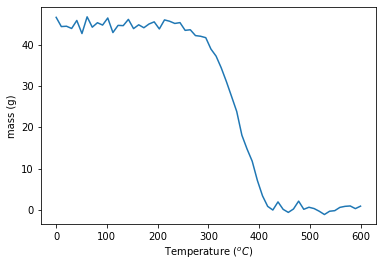
\includegraphics[scale=1]{figures/bayesian/Noisy_tga.png}
\caption{Sample noisy experimental data.}
\label{fig:single_mass}
\end{figure}

The random sample of parameter estimates obtained through the MCMC algorithm are displayed in Figures \ref{HistA} and \ref{HistE}. These histograms are indicative of the posterior distribution. We can use this data to analyse the posterior distribution to obtain point estimates and confidence intervals for the parameters. The ability to apply a functional transformation of our sampled data allows us to utilise these estimates for $\tilde{A}$ and $\tilde{E}$ to determine the critical stockpile lengths required for stockpile ignition. This is a significant advantage of the Bayesian approach. \\ 
\begin{figure}[h!]
\centering
\begin{subfigure}{0.5\textwidth}
\centering
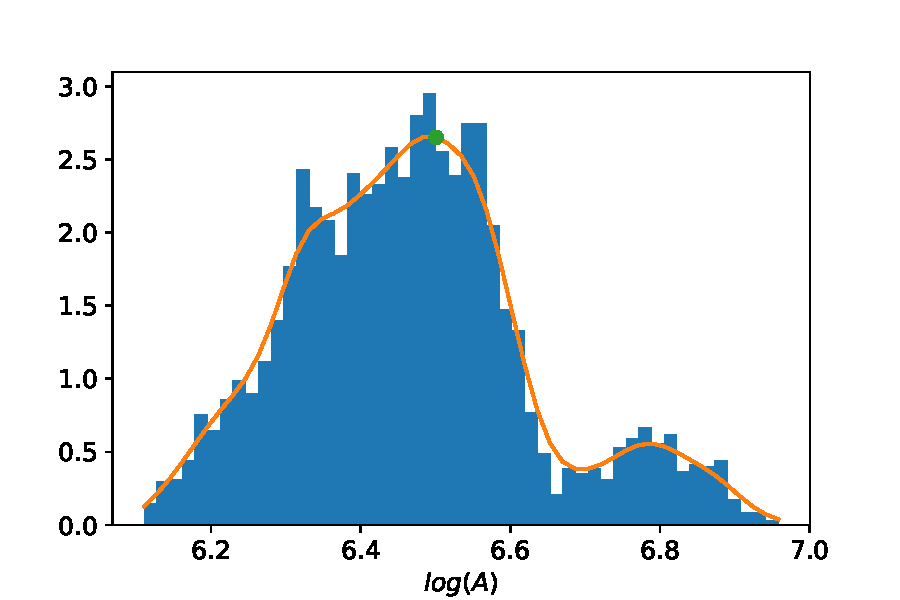
\includegraphics[width=\linewidth]{figures/bayesian/hist_A.pdf}
\caption{Histogram of $\tilde{A}$.}
\label{HistA}
\end{subfigure}%
\begin{subfigure}{0.5\textwidth}
\centering
\includegraphics[width=\linewidth]{figures/bayesian/hist_E.pdf}
\caption{Histogram of $\tilde{E}$.}
\label{HistE}
\end{subfigure}
\newline
\begin{subfigure}{0.5\textwidth}
\centering
\includegraphics[width=\linewidth]{figures/bayesian/hist_sigma.pdf}
\caption{Histogram of $\sigma$.}
\label{Histsigma}
\end{subfigure}%
\begin{subfigure}{0.5\textwidth}
\centering
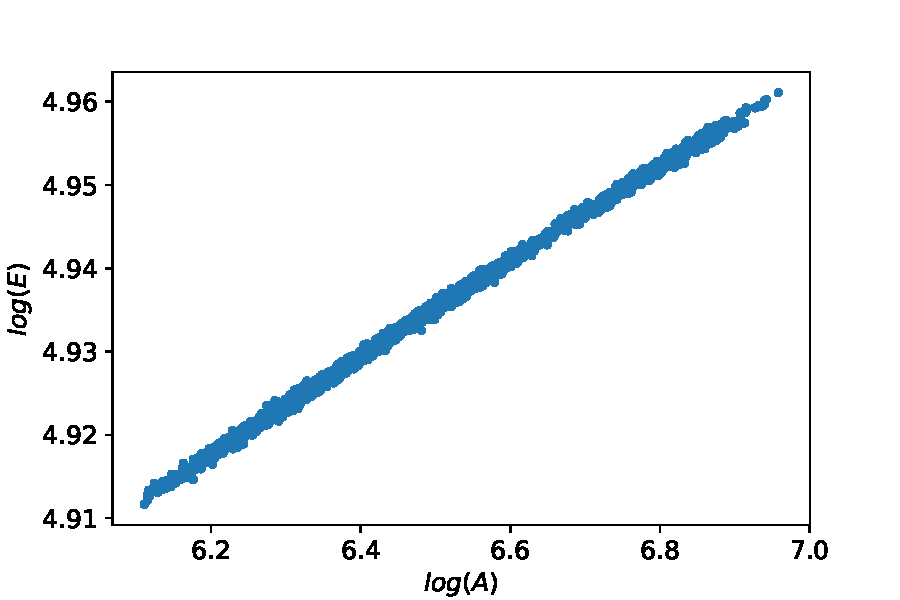
\includegraphics[width=\linewidth]{figures/bayesian/joint_distribution.pdf}
\caption{Joint distribution of $\tilde{A}$ and $\tilde{E}$.}
\label{AvsE}
\end{subfigure}
\caption{Output from the Metropolis-Hastings algorithm with the true values indicated.}
\label{fig:MH1}
\end{figure}

Figure \ref{fig:MH1} displays the sample density that our Metropolis-Hastings Algorithm generates. In each Histogram we capture the true value within the bounds of our sample. We can construct confidence intervals for the true parameters based off our samples. Given we have the true values we can calculate the percentile of each value and these are stated in Table \ref{tab:MH1}. Various summary statistics were calculated and can be found in Appendix \ref{App:1_Summary}.\\ 
\begin{table}[h!]
\centering
\begin{tabular}{|c|c|c|}
\hline 
Parameter & True Value & Percentile \\
\hline
$\tilde{E}$ & 4.94 & 89.7 \\
\hline
$\tilde{A}$ & 6.5 & 89.5 \\
\hline
$\sigma$ & 0.05 & 0\\
\hline
\end{tabular}
\caption{Table of the percentile scores from the Metropolis-Hastings Algorithm.}
\label{tab:MH1}
\end{table}

%Add figure for the histogram of Sigma.
Figure \ref{Histsigma} indicates that the 4 chains have not converged and that no chain has estimated the true noise. This presents a major issue with our algorithm. Figure \ref{fig:trace1} displays the trace plots for the parameters $\tilde{A}$ and $\tilde{E}$. The figure indicates that some chains take significantly longer to converge. This causes issues in determining the appropriate number of samples to accept before terminating the algorithm. This is also a reason why the sigma values are comparatively large. If the sampled points produce a FWC curve that is not sufficiently close to the data, then increasing the noise parameter increases the likelihood. Additional figures for the trace plots of each parameter are included in Appendix \ref{App:1_traces}.
\begin{figure}[h!]
\centering
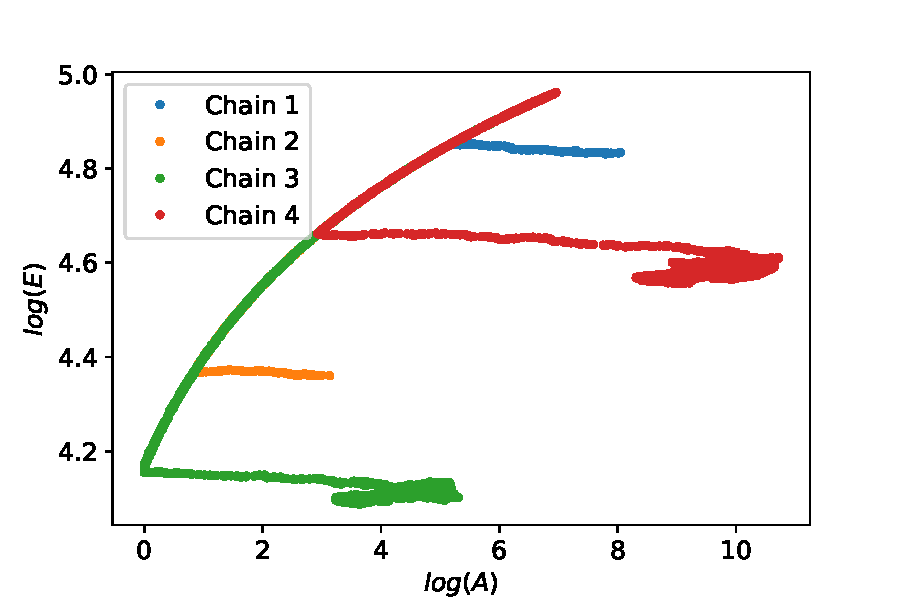
\includegraphics[width=\linewidth]{figures/bayesian/trace_plots.pdf}
\caption{Trace plots of the parameters $\tilde{A}$ and $\tilde{E}$, for each chain.}
\label{fig:trace1}
\end{figure}

Figure \ref{AvsE} plots the joint distribution of the parameters $\tilde{E}$ and $\tilde{A}$. This indicates that the two variables are highly correlated, with correlation coefficient, $0.99$. The fact that the variables are highly correlated causes inefficiencies in the MCMC algorithm.
Given that this curve is so signifant in the acceptance of new data points, it is useful to design an algorithm that samples along this curve. When we propose $\tilde{A}$ and $\tilde{E}$ independently, it is unlikely to remain on this curve.\\
Consider Equation \ref{eqkis},
\begin{equation}
A\exp\left(\frac{-E}{RT_m}\right)=\frac{E}{RT_m^2}\frac{dT}{dt}, \label{eqkis}
\end{equation}
derived in section \ref{SEC:TGA}.
This equation relates the pre-exponential factor ,$A$, and activation energy, $E$, to the temperature at which the reaction rate is maximised, $T_m$. Figure \ref{fig:eqkis_comp} compares the points sampled by our original algorithm with the theoretical true curve with $T_{m,\text{true}}=635$K. We observe that the Markov Chains follow this curve quite closely. Using this information it would be more beneficial to propose new parameters along these curves. The issue remains in how to identify which of these curves do we sample along.\\
\begin{figure}[h!]
\centering
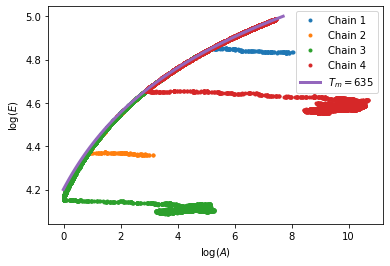
\includegraphics[width=\linewidth]{figures/bayesian/Theoritcal_Tm.png}
\caption{A comparison of the sampled points and the curve in equation \ref{eqkis}.}
\label{fig:eqkis_comp}
\end{figure}

Using Equation \ref{eqkis} alleviates another issue with our sampling method; We do not have good prior information on either the pre-exponential factor nor the activation energy. This equation allows us to replace the parameter $\tilde{A}$ from our sample space with the parameter $T_m$. We propose $T_m$ and $\tilde{E}$ values, and then using Equation \ref{eqkis} we determine the corresponding $\tilde{A}$ value. In the case where we have one reaction, we can often measure $T_m$ directly from the experimental data. For this simulation we do not wish to use this explicit value as we intend to apply this to a scenario with two reactions where we are unable to determine the value explicitly. Even without knowing the exact value, we are able to obtain a useful prior distribution for $T_m$. We use a uniform prior with a limited range.\\
%Include additional figures for the new histograms. Also provide histograms for the original parameters.
\begin{figure}[h!]
\centering
\begin{subfigure}{0.5\textwidth}
\centering
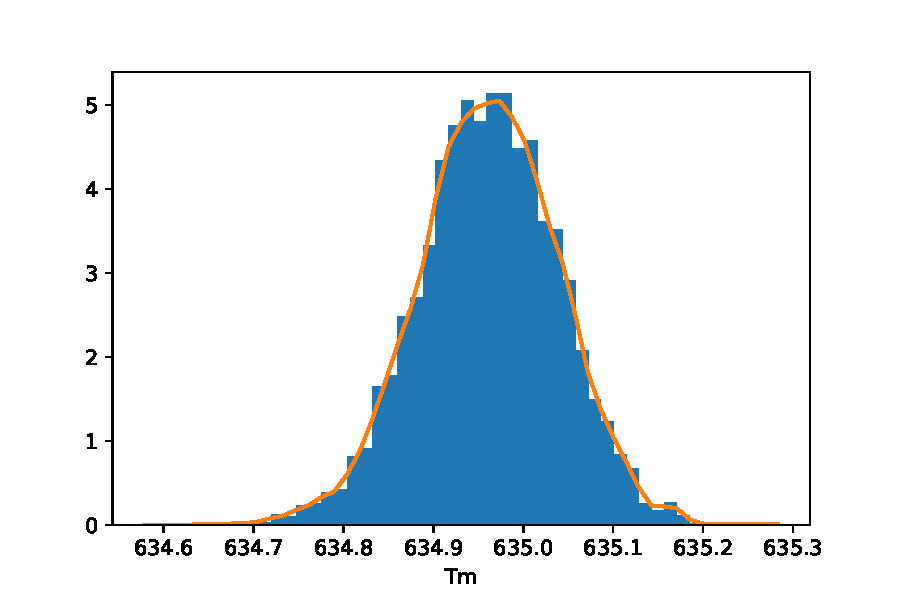
\includegraphics[width=\linewidth]{figures/bayesian/Tm/hist_Tm.pdf}
\caption{Histogram of $T_m$}
\label{HistTm}
\end{subfigure}%
\begin{subfigure}{0.5\textwidth}
\centering
\includegraphics[width=\linewidth]{figures/bayesian/Tm/hist_E.pdf}
\caption{Histogram of $\tilde{E}$}
\label{HistTE}
\end{subfigure}
\newline
\begin{subfigure}{0.5\textwidth}
\centering
\includegraphics[width=\linewidth]{figures/bayesian/Tm/hist_sigma.pdf}
\caption{Histogram of $\sigma$}
\label{HistTsigma}
\end{subfigure}%
\begin{subfigure}{0.5\textwidth}
\centering
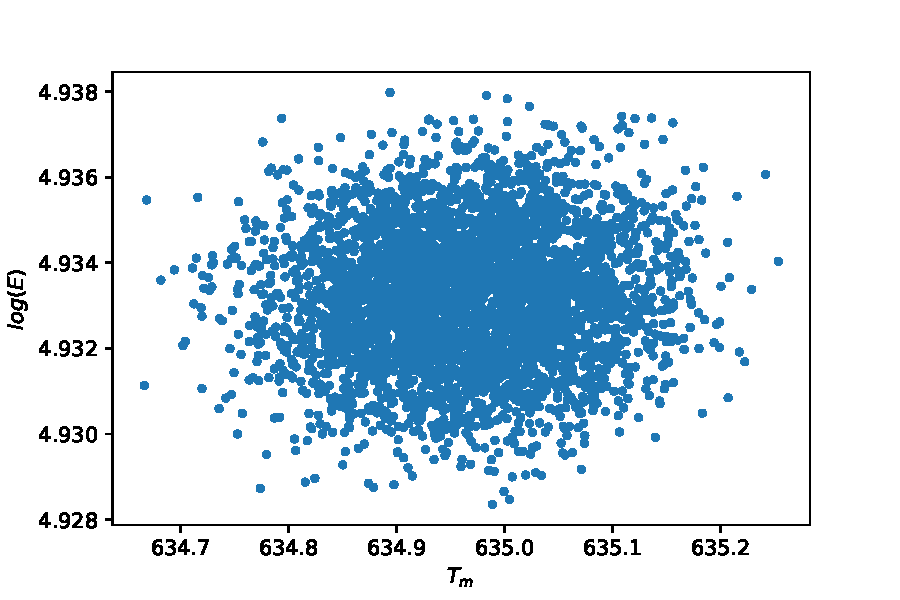
\includegraphics[width=\linewidth]{figures/bayesian/Tm/joint_distribution.pdf}
\caption{Joint distribution of $T_m$ and $\tilde{E}$.}
\label{TvsE}
\end{subfigure}
\caption{Output from the Metropolis-Hastings algorithm using the parameters $(T_m,E)$, with the true values indicated.}
\label{fig:MH2}
\end{figure}

%Look to include traceplots and additional information on
Using the parameter $T_m$, we obtain very similar graphs for $A$ and $E$. The plot for $E$ against $T_m$ is displayed in figure \ref{TvsE}. This figure indicates that there is no significant correlation between the two parameters. This is useful in our algorithm as it improves the acceptance rate with similar step sizes. This is further supported by the trace plot in figure \ref{fig:trace2}.\\
\begin{figure}[h!]
\centering
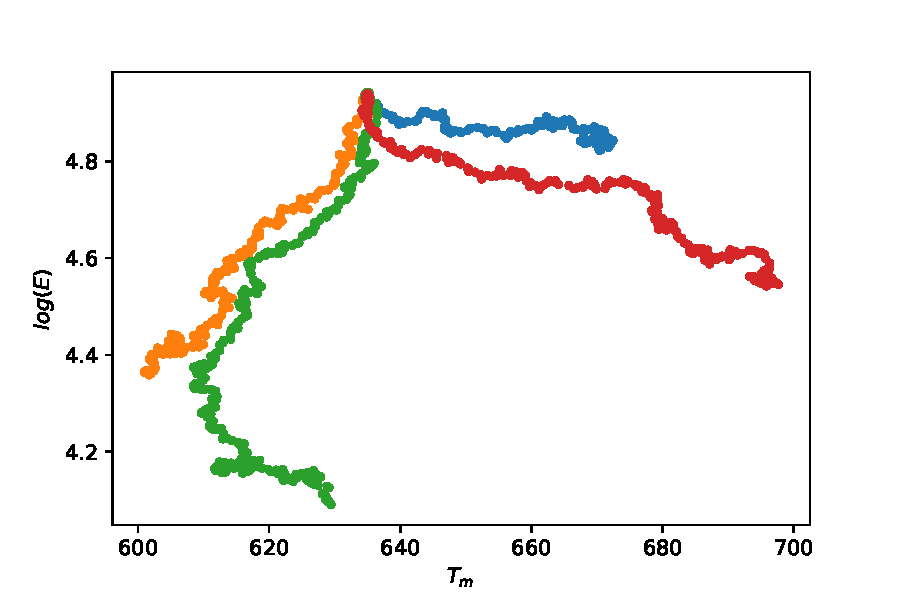
\includegraphics[width=\linewidth]{figures/bayesian/Tm/trace_plots.pdf}
\caption{Trace plots of the parameters $T-m$ and $\tilde{E}$, for each chain.}
\label{fig:trace2}
\end{figure}
One of the key metrics we are interested in is the effect that this variation has on the predicted critical length of the stockpile. This is a major benefit of the MCMC approach as we can conduct a functional transform from our sample to the critical length using the formula,
\begin{equation}
L_{cr}=K \sqrt{\frac{\exp\left(\frac{E}{RT_a^2}\right)}{A}\frac{RT_a^2}{E}},
\label{eq:Lcr}
\end{equation}
where $K$ is some constant that depends upon various constants in our stockpile model. Equation \ref{eq:Lcr} was derived in Section \ref{SEC:Lcr}. We have taken this constant such that the minumum critical length is $1$m.
Figure \ref{fig:HistL} indicates that the critical length of the stockpile can be determined to within some reasonable range. The values in the histogram are indicative of the critical lengths and are dependant on the thermal conductivity and the heat of reaction; these parameters are not included in our TGA analysis. Using Equation \ref{eq:Lcr} and taking logarithms we obtain,
\begin{equation}
\log \left(L_{cr}\right)=\log (K)+\log\left(\frac{RT_a^2}{EA}\right) +\frac{E}{RT_a^2}\log( e).
\end{equation}
This form clearly indicates that the parameter, $K$ shifts the values of $\log L_{cr}$ and does not affect the spread.\\
\begin{figure}
\centering
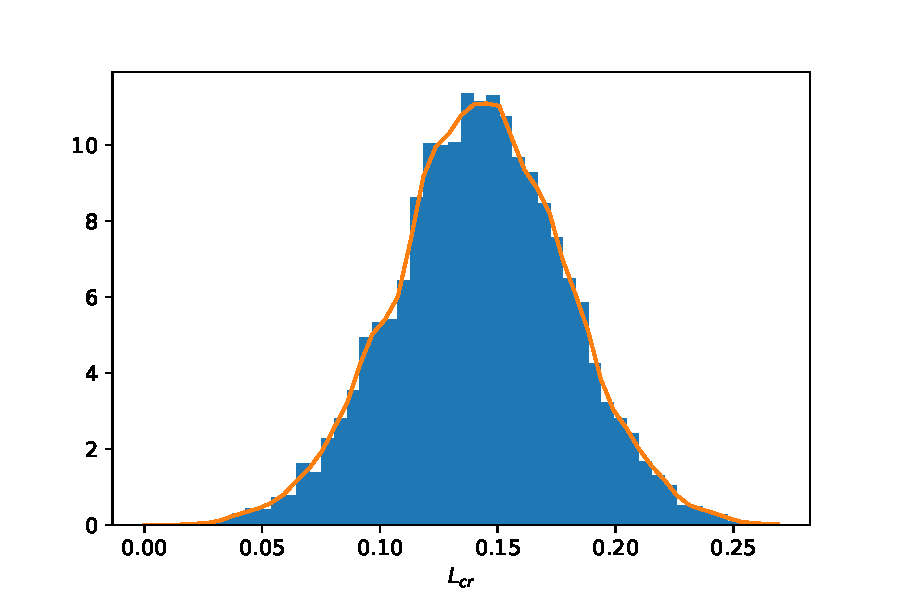
\includegraphics[scale=1]{figures/bayesian/hist_Lcr.pdf}
\caption{Histogram of the sample obtained for $\log_{10}\left(L_{\text{cr}}\right)$ through the MCMC algorithm.}
\label{fig:HistL}
\end{figure}
\subsubsection{Selecting Appropriate Parameters}
This section has shown that utilising a different set of parameters can improve the efficiency of the MCMC algorithm. It is useful to consider why this is the case.\\ 
\begin{figure}[h!]
\centering
\begin{subfigure}{.5\textwidth}
  \centering
  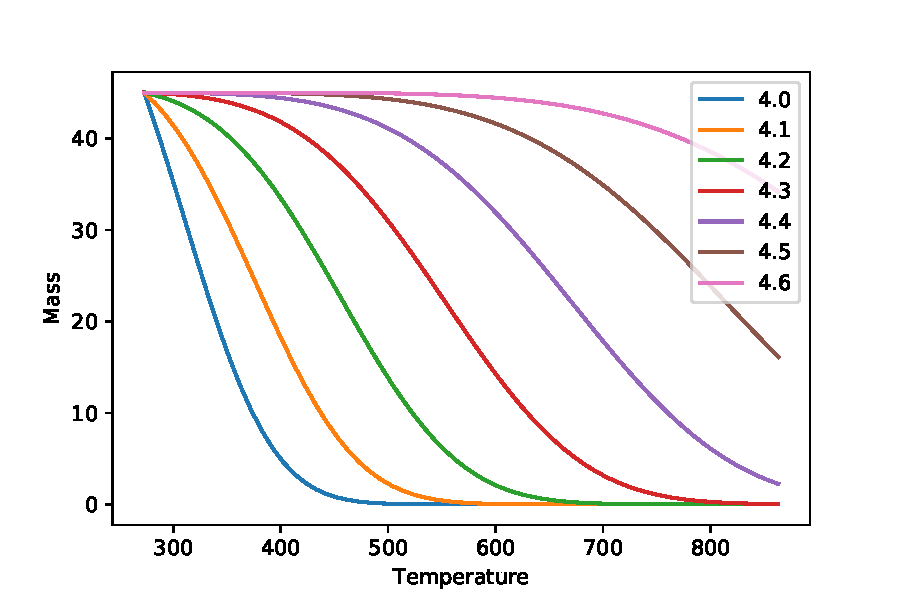
\includegraphics[width=\linewidth]{figures/bayesian/1_reaction/E_A_fwc.pdf}
  \caption{The effect of $\tilde{E}$ with $\tilde{A}=6$.}
  \label{fig:subfwc_E_A}
\end{subfigure}%
\begin{subfigure}{.5\textwidth}
  \centering
  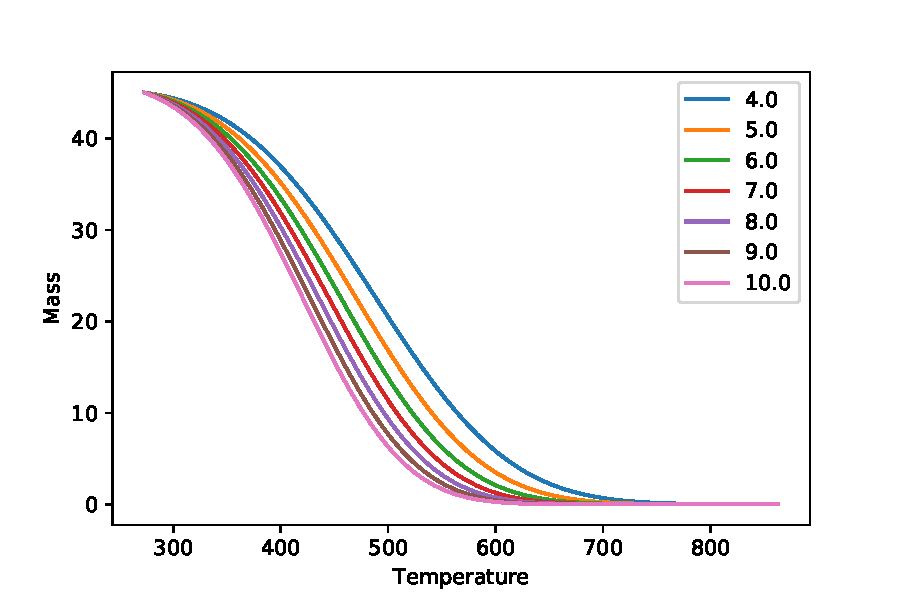
\includegraphics[width=\linewidth]{figures/bayesian/1_reaction/A_fwc.pdf}
  \caption{The effect of $\tilde{A}$ with $\tilde{E}=4.2$.}
  \label{fig:subfwc_A_E}
\end{subfigure}
\newline
\begin{subfigure}{.5\textwidth}
  \centering
  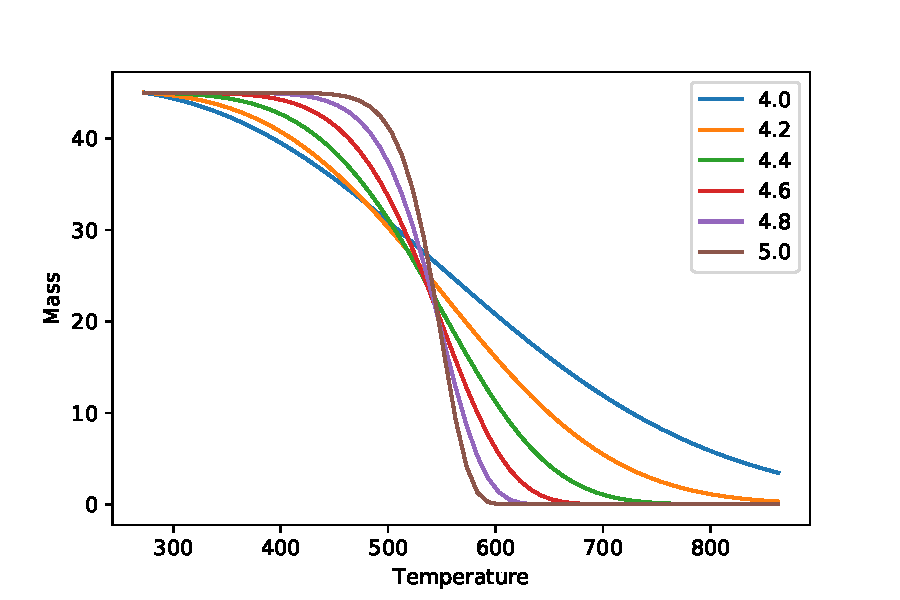
\includegraphics[width=\linewidth]{figures/bayesian/1_reaction/E_fwc.pdf}
  \caption{The effect of $\tilde{E}$ with $T_m=550$.}
  \label{fig:subfwc_E_Tm}
\end{subfigure}%
\begin{subfigure}{.5\textwidth}
  \centering
  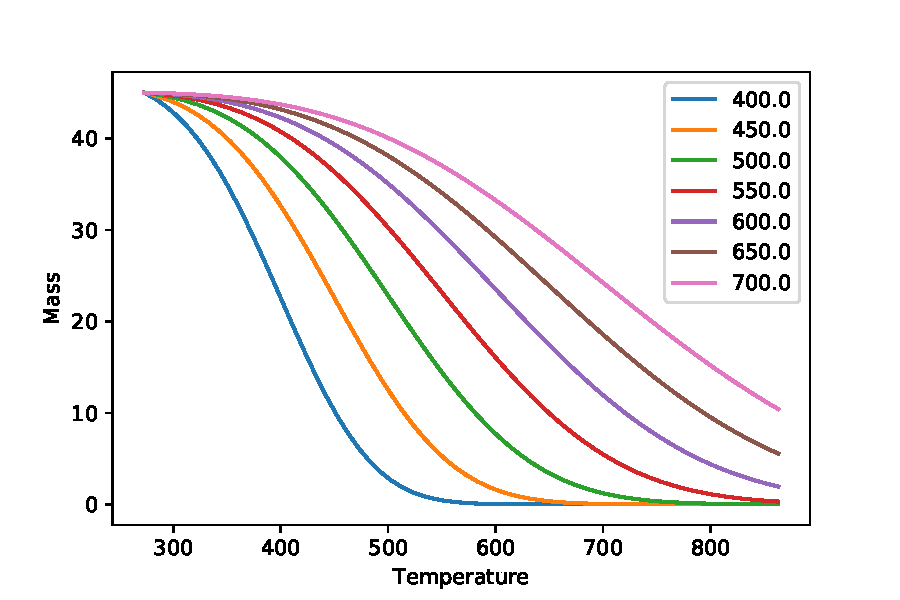
\includegraphics[width=\linewidth]{figures/bayesian/1_reaction/Tm_fwc.pdf}
  \caption{The effect of $T_m$ with $\tilde{E}=4.2$.}
  \label{fig:subfwc_Tm_E}
\end{subfigure}
    \caption{Comparison of the effects of each parameter pairing on the FWC curve.}%
    \label{fig:FWC_para_comp}%s}
\end{figure}%
Figure \ref{fig:FWC_para_comp} demonstrates the effect that altering each parameter has on the FWC curve. We observe in figures \ref{fig:subfwc_E_A} and \ref{fig:subfwc_A_E}, that the $\tilde{E}$ parameter has a large effect on both when the reaction occurs and its duration; small changes in $\tilde{E}$ cause a large shift in the FWC curve. In contrast the affect of changing $\tilde{A}$ appears to be minimal. Dramatically changing the order of magnitude of the parameter has little effect on FWC curve. This is in contrast to the $\left(\tilde{E},T_m\right)$ pairing displayed in figures \ref{fig:subfwc_E_Tm} and \ref{fig:subfwc_Tm_E}. In this set up, $T_m$ is the sole indicator of the reaction's location. As $T_m$ is increased, the duration of the reaction increases. The key difference is that as we vary $\tilde{E}$ the location of the reaction remains the same; only the duration of the reaction changes. It is important to note the the temperature ranges from 400 to 700 K, which is far greater than any prior information will deem necessary. This is a key observation in increasing the efficiency as we are able to start the algorithm with a useful prior for $T_m$ and the small changes in $T_m$ do not cause large changes in the duration of the reaction. This enables the parameter $\tilde{E}$ to control the duration whilst $T_m$ refines the location.\\
Figure \ref{fig:FWC_para_comp} displays graphically why the parameter pairing $\left(\tilde{E},T_m\right)$ can be considered a better basis than the parameter pairing $\left(\tilde{E},\tilde{A}\right)$.

\subsection{Application to Experimental Data}
\label{Sec:1R_EXP}
We can apply this algorithm to an experimental dataset where only a single reaction is occuring. This is a very simple experiment that serves to test the algorithm on experimental data where the underlying parameters are unknown. We model our reactant using equation \ref{TGA_system_BI},
\begin{align*}
\frac{dM}{dt}&=-MOA\exp\left(\frac{-E}{RT}\right), \\
\frac{dT}{dt}&=\alpha. 
\end{align*}
This models the mass of the reactant, whereas the experimental data is in terms of a mass percentage. Since our model is invariant for mass we can scale this by the initial mass, without affecting any of the other parameters. We determine the mass percentage using the equation,
\begin{equation}
SM=M+\frac{M_f}{M_0}\left(M_0-M\right),
\end{equation}
where $M_f$, is the final mass, $M_0$, is the initial mass, and $SM$ is the sample mass as a percentage of the initial mass. This equation is a sum of the mass of reactant, $M$, and the product mass $\frac{M_f}{M_0}\left(M_0-M\right)$. This approach assumes that sample is pure and the reaction is complete at the end of the experiment; This is valid with our data. The fractional weight change data is presented in Figure \ref{fig:FWC_exp}. For our analysis, we restrict the data to the window wher the temperature is between $250^oC$ and $1250^oC$. This reduces some complications initially where the sample is not heated at a constant rate, and removes the back end of the reaction where the mass change is negligible.\\

\begin{figure}[h!]
\centering
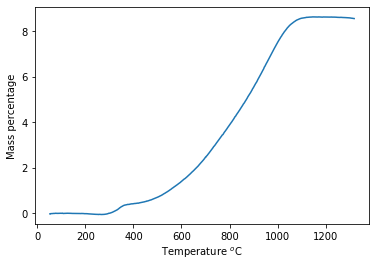
\includegraphics[scale=0.75]{figures/bayesian/1_reaction/EXP/FWC_data.png}
\caption{The FWC curve for a simple experiment where one reaction is occuring.}
\label{fig:FWC_exp}
\end{figure}

We will introduce a variable proposal distribution into our algorithm. The prior information we have in determining the temperature where the reaction rate is maximised, is less precise than our simulated examples. This requires a larger step size initially to explore this space, though we still require a narrower proposal once the chains have converged to efficiently sample the posterior. To implement this our proposal is $N\left(\theta_{t-1},\frac{s}{\sqrt{d}}\right)$, where, $s$ is our fixed proposal standard deviation, and $d$ is our control parameter. We simulate for 20000 iterations total and after we reach 10000 iterations we increase the parameter $d$, narrowing the proposal distribution.\\ 
\begin{figure}[h!]
\centering
\begin{subfigure}{.5\textwidth}
  \centering
  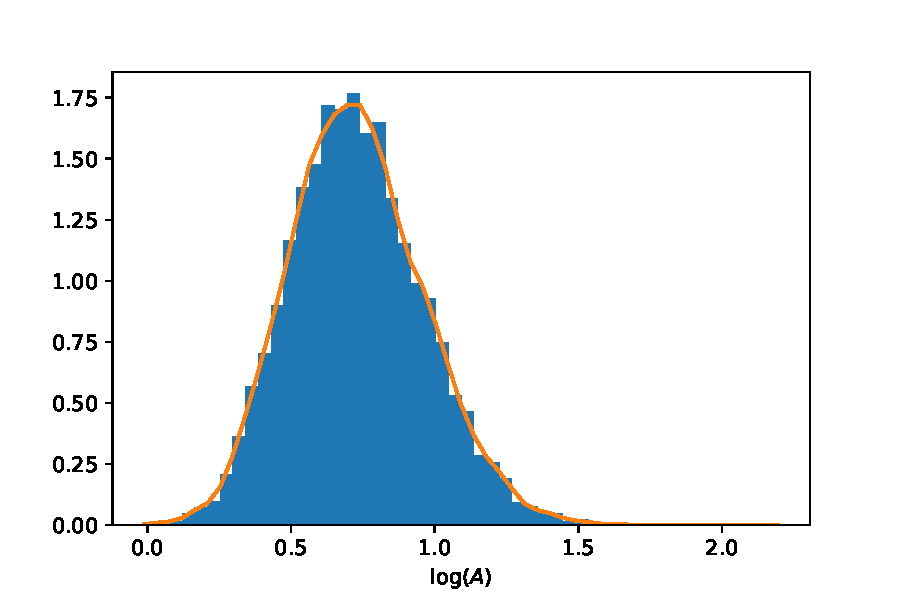
\includegraphics[width=\linewidth]{figures/bayesian/1_reaction/EXP/hist_A.pdf}
  \caption{Histogram of $\tilde{A}$.}
  \label{fig:1EXPA}
\end{subfigure}%
\begin{subfigure}{.5\textwidth}
  \centering
  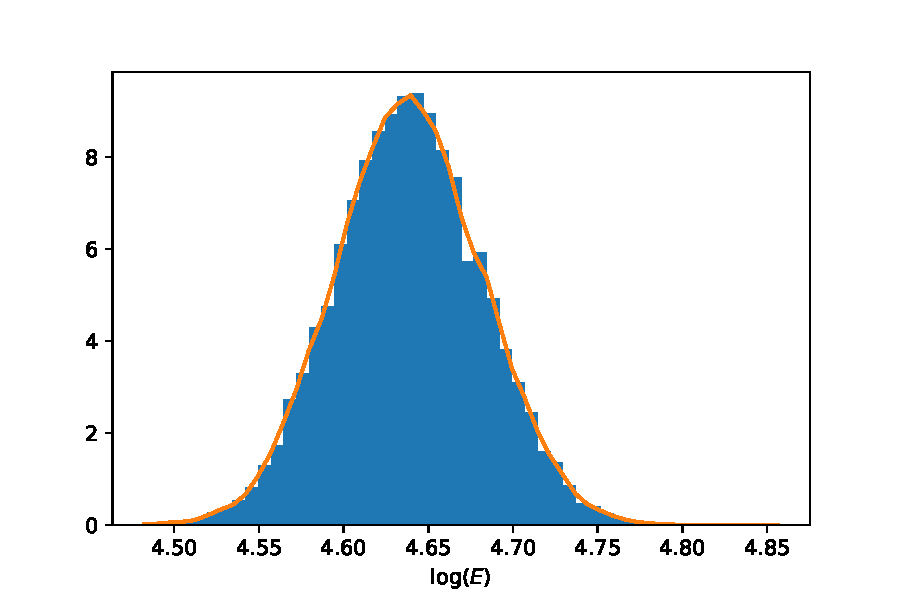
\includegraphics[width=\linewidth]{figures/bayesian/1_reaction/EXP/hist_E.pdf}
  \caption{Histogram of $\tilde{E}$.}
  \label{fig:1EXPE}
\end{subfigure}
\newline
\begin{subfigure}{.5\textwidth}
  \centering
  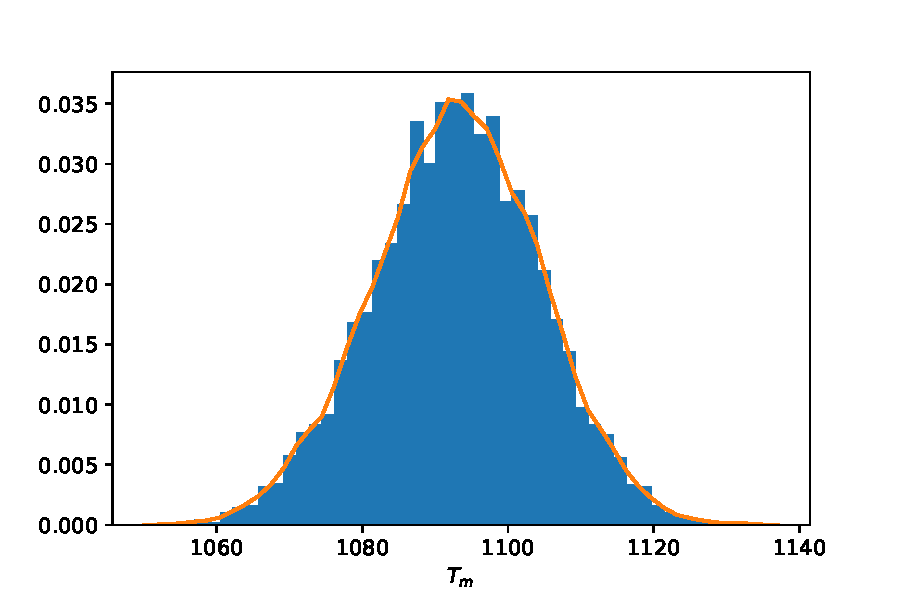
\includegraphics[width=\linewidth]{figures/bayesian/1_reaction/EXP/hist_Tm.pdf}
  \caption{Histogram of $T_m$.}
  \label{fig:1EXPTm}
\end{subfigure}%
\begin{subfigure}{.5\textwidth}
  \centering
  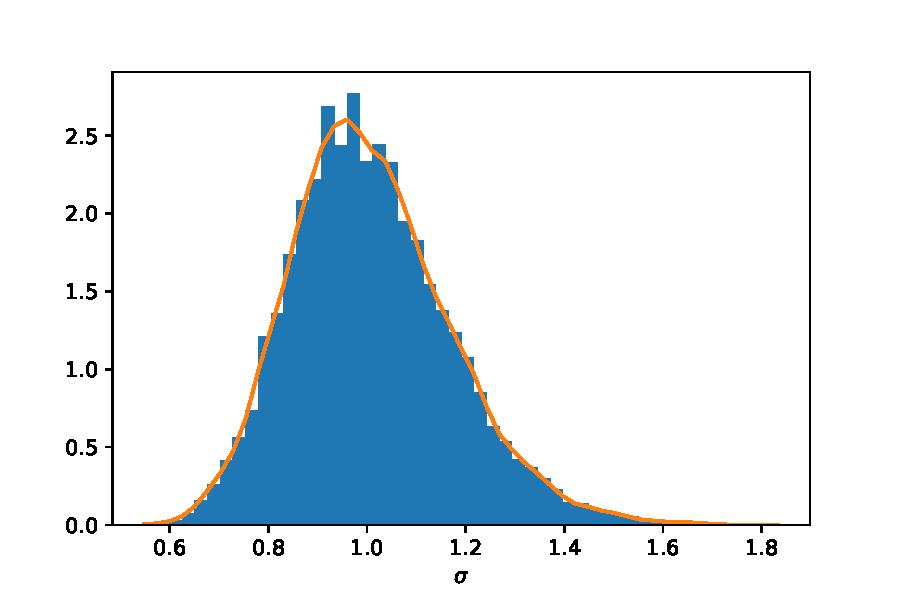
\includegraphics[width=\linewidth]{figures/bayesian/1_reaction/EXP/hist_sigma.pdf}
  \caption{Histogram of $\sigma$.}
  \label{fig:1EXPsigma}
\end{subfigure}
    \caption{Histograms of sampled parameters of the posterior distribution for the experimental data.}%
    \label{fig:EXP1}%s}
\end{figure}%

Figure \ref{fig:EXP1} displays the samples samples from the posterior distribution. This figure indicates that we have a large uncertainty within our parameters. When examining the trace plots in Figure \ref{fig:EXPtrace}, the algorithm behaves as we expect. These trace plots include the first 10000 points sampled which are discarded as burnin. We also observe that the variance in the noise $\sigma$, is much higher than in our simulated examples and is higher than we expect for the experimental data. This suggests that there may be an issue with model misspecification.\\

\begin{figure}[h!]
\centering
\begin{subfigure}{.5\textwidth}
  \centering
  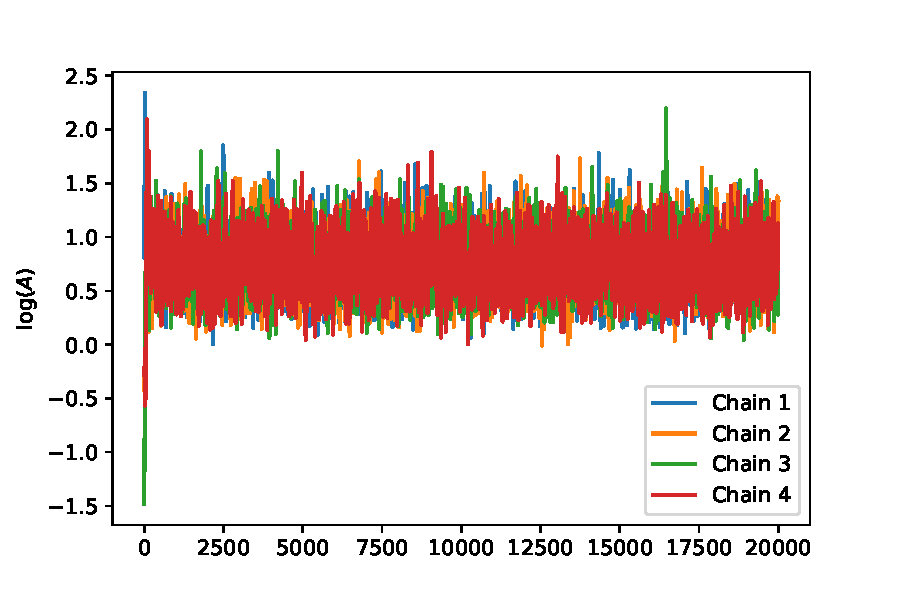
\includegraphics[width=\linewidth]{figures/bayesian/1_reaction/EXP/trace_plot_A.pdf}
  \caption{Trace plot of $\tilde{A}$.}
  \label{fig:1EXPA}
\end{subfigure}%
\begin{subfigure}{.5\textwidth}
  \centering
  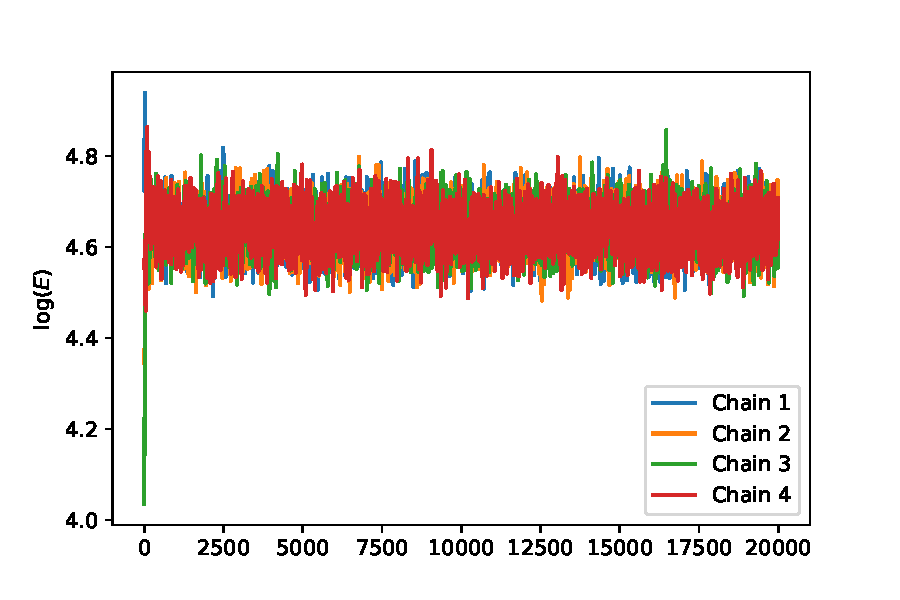
\includegraphics[width=\linewidth]{figures/bayesian/1_reaction/EXP/trace_plot_E.pdf}
  \caption{Trace plot of $\tilde{E}$.}
  \label{fig:1EXPE}
\end{subfigure}
\newline
\begin{subfigure}{.5\textwidth}
  \centering
  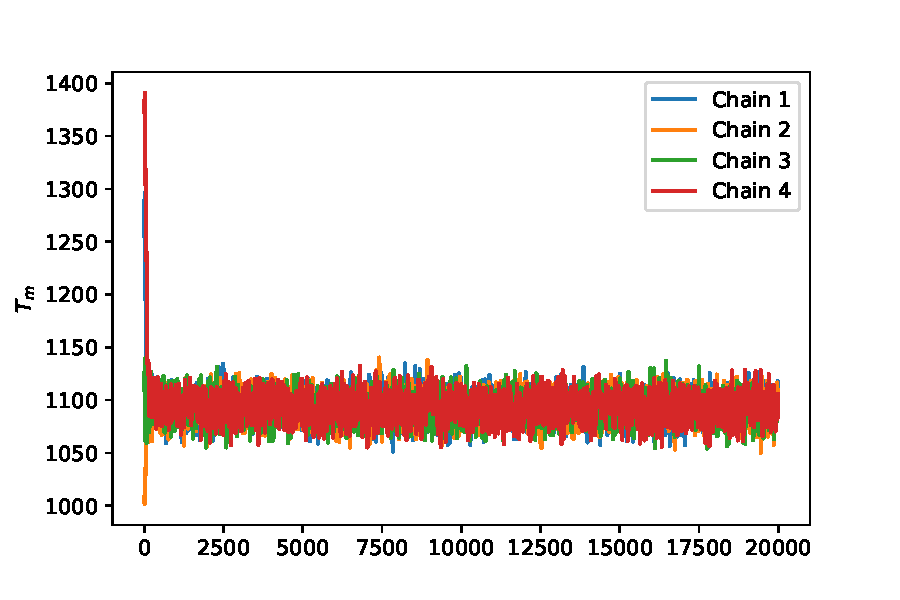
\includegraphics[width=\linewidth]{figures/bayesian/1_reaction/EXP/trace_plot_Tm.pdf}
  \caption{Trace plot of $T_m$.}
  \label{fig:1EXPTm}
\end{subfigure}%
\begin{subfigure}{.5\textwidth}
  \centering
  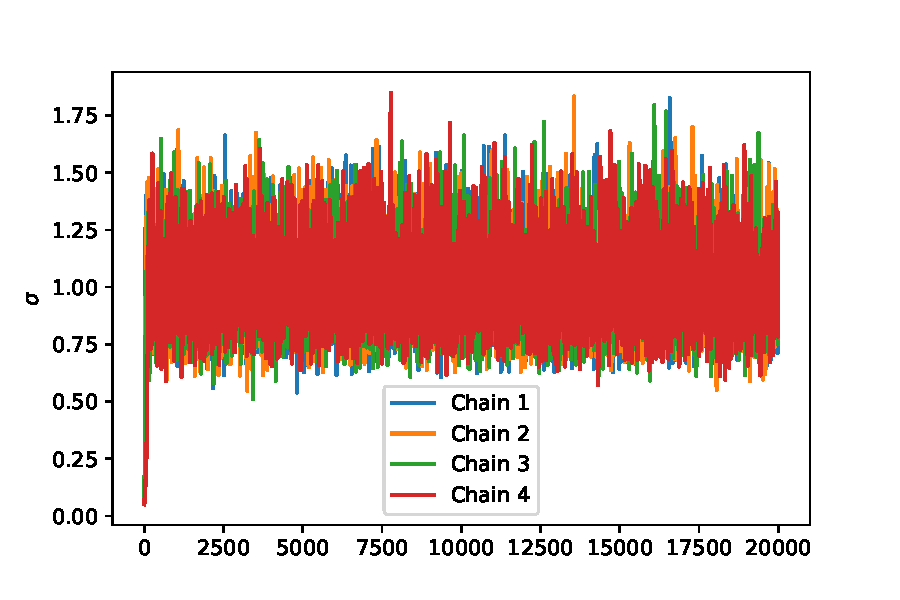
\includegraphics[width=\linewidth]{figures/bayesian/1_reaction/EXP/trace_plot_sigma.pdf}
  \caption{Trace plot of $\sigma$.}
  \label{fig:1EXPsigma}
\end{subfigure}
    \caption{Trace plots for each of the parameters of our MCMC algorithm applied to experimental data.}%
    \label{fig:EXPtrace}%s}
\end{figure}%

To examine the hypothesis that the model doesn't accurately represent the data, we plot some of the sampled curves. We randomly select 10 data points and simualte the experiment and plot them all against the FWC data. What we observe in Figure \ref{fig:comp_exp}, is that the FWC curves find this other mode. What is also worth noting, is that it is difficult to say which curve is a better fit for the data. This is expected through our algorithm. The data has an unusual structure early in the reaction that is likely causing some of these issues.\\

\begin{figure}[h!]
\centering
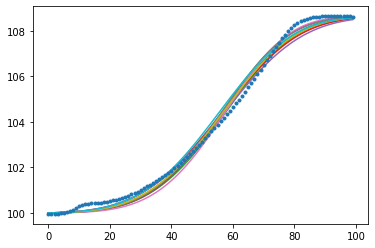
\includegraphics[width=\linewidth]{figures/bayesian/1_reaction/EXP/example_curve.png}
\caption{A random sample of FWC curves against the experimental data.}
\label{fig:comp_exp}
\end{figure}

\begin{figure}[h!]
\centering
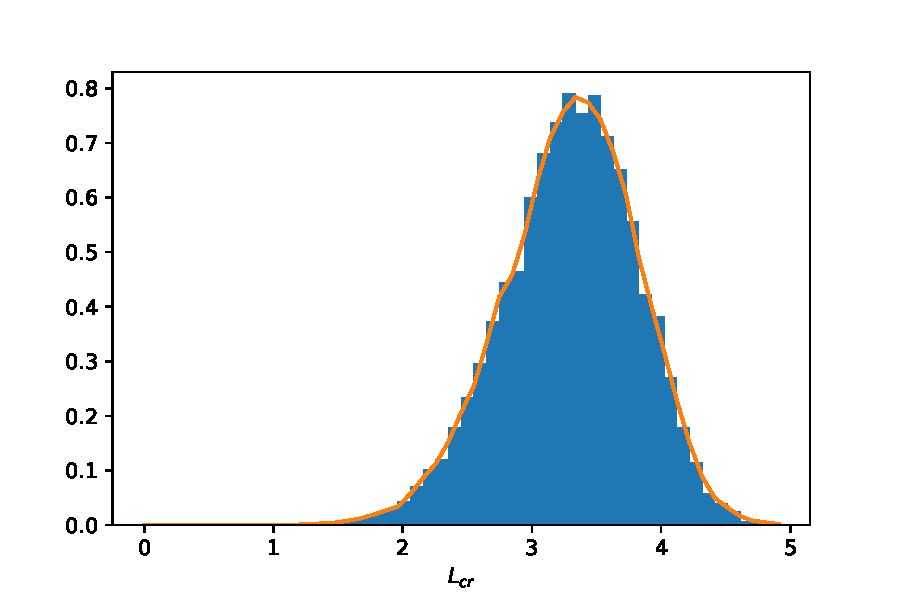
\includegraphics[width=\linewidth]{figures/bayesian/1_reaction/EXP/hist_Lcr.pdf}
\caption{Histogram of the logarithm of the critical length of the stockpile made from the material in the experiment.}
\label{fig:Lcr_exp}
\end{figure}

Persisting with this model we are able to sample from the posterior of the critical length of a stockpile to be built with this material. Figure \ref{fig:Lcr_exp} indicates that the critial length varies over many orders of magnitude. This indicates that using any of these acceptable curves in Figure \ref{fig:comp_exp} in isolation, could provide a poor estimate of the critical length needed for ignition to occur. This highlights the need for consideration of the uncertainty of parameters in assessing models. This analysis indicates that if we wish to approximate the reactions using this model, then we have a large uncertainty within our parameters, and this causes a large uncertainty in the critical length of the stockpiles. To avoid this issue, then we need additional data, or to use an alternative model that can better predict this behaviour. This simple example also indicates the dangers we could face if we use a simple one reaction model as an approximation for more complicated reaction schemes.\\



\section{Two Reactions}
Now that we have an algorithm set up for a single reaction, we extend this to two parallel reactions. For the identifiability of the parameters, we need to ensure the reactions maintain a defined order. Experimentally we can determine which of the two reactions is occurring first, as such the simulations need to reflect this.\\ 

To model the experiment we use the equation defined in equation \ref{FWC_equation},
\begin{equation}
\frac{dM_t}{dt}=w_{c,1}M_1A_1\exp\left(\frac{-E_1}{RT}\right)+w_{c,2}M_2A_2\exp\left(\frac{-E_2}{RT}\right). \label{FWC_equation}
\end{equation}
This equation simplifies down to the equation,
\begin{equation}
M_t=M_{t_0}+w_{c,1}\left(M_1-M_{1_0})\right)+w_{c,2}\left(M_2-M_{2_0})\right),
\end{equation}
where the $0$ subscript denotes the initial masses. The masses, $M_1$ and $M_2$ follow Equation \ref{TGA_system_BI}. We use this weight change equation as it best mimics the experiments that have been conducted. For the statistical model, Equation \ref{FWC_equation}, is used to determine the theoretical solution, which we discretise at given times, $t$. We then add Gaussian noise to our simulated solution.
As our results for the one reaction case indicate that it is better to estimate $T_m$ then we shall explore that parameter space for the two reaction model. We initially consider a scheme with well seperated reactions. The true parameters for our parameter space are defined in table \ref{sim_paras}.\\
For the two reaction models we adjust our algorithm as well. As we introduce more complex behaviour into our model, then efficiency becomes more of an issue. We observed in the one reaction model, that the algorithms can take a significant time to converge. This is computationally inefficient. We also still want our algorthm to have an acceptance rate of approximately $0.234$. As such we divide our algorithm into three stages. Initially we propose from a Gaussian distribution with high variance. In this stage we anticipate the acceptance rate can vary dramatically, but once the optimal node is found, then we will have a low acceptance rate. The intermediate stage has a more narrow proposal distribution where the algorithm refines this node further. The final stage is where we obtain our sample. In this region the algorithm is expected to have converged, so the proposal distribution can be altered to achieve an acceptance rate around the optimal value.\\ 

\begin{table}[h!]
\centering
\begin{tabular}{|c|c|}
\hline
Parameter & value \\ \hline
$E_1$ & $8.6 \times 10^4$ J/mol \\ \hline
$E_2$ & $2.6 \times 10^5$ J/mol\\ \hline
$T_{m,1}$ & 560 K\\ \hline
$T_{m,2}$ & 750 K\\ \hline
$A_1$ & $3.5 \times 10^7 $ m$^3$/kg/s\\ \hline
$A_2$ & $7.1 \times 10^{17} $ m$^3$/kg/s \\ \hline
$\sigma$ & 0.05 \\ \hline
\end{tabular}
\caption{Parameter values for the simulation.}
\label{sim_paras}
\end{table} 

When need to introduce some constraint such that the reactions correspond to the correct portion of the data. Each of the reactions contribute independently to the overall FWC curve. Given that experimentally we can determine which reaction is peaking earlier than our model needs to preserve this. We enforce this constraint through including an informative prior. In our prior we have an additional constraint that $T_{m,1}<T_{m,2}$. We enforce this by using uniform distributions on non-overlapping domains. When the two peaks become closer, we consider a joint prior that enforces this condition.\\

Following Algorithm \ref{Alg:MH}, the samples are presented in Figure \ref{fig:MH3}. These histograms indicate that the chains have converged. The trace plots for these chains also indicate this and can be found in Appendix \ref{App:2_traces}. When we compare these histograms to those in Figure \ref{fig:MH2}, then we observe a similar variances occurring though with two reactions it increases slightly. Interestingly, our sample does not include the true values for $T_{m,2}$ and $\tilde{A_2}$.\\

\begin{figure}[h!]
\centering
\begin{subfigure}{0.5\textwidth}
\centering
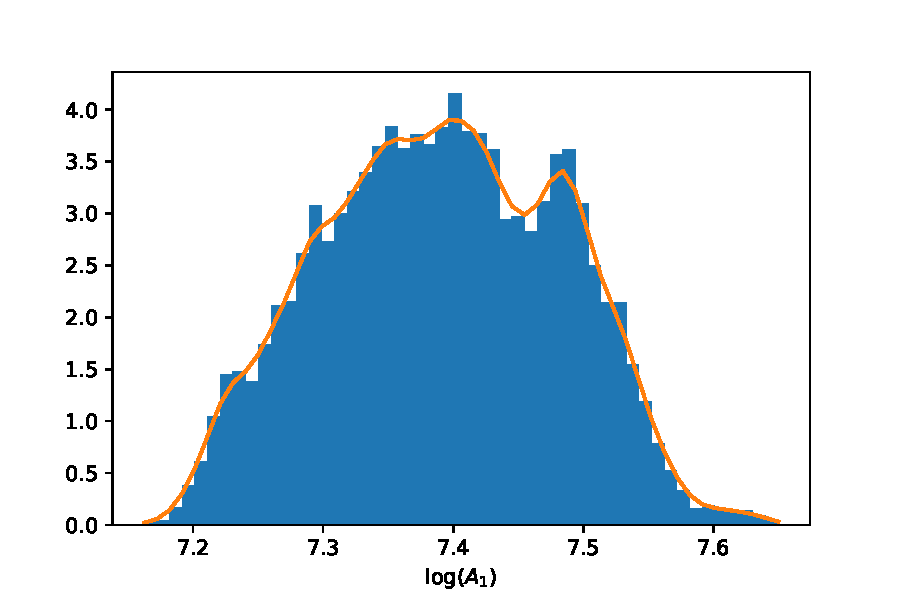
\includegraphics[width=\linewidth]{figures/bayesian/2_reactions/mass/hist_A1.pdf}
\caption{Histogram of $\tilde{A_1}$.}
\label{HistA1}
\end{subfigure}%
\begin{subfigure}{0.5\textwidth}
\centering
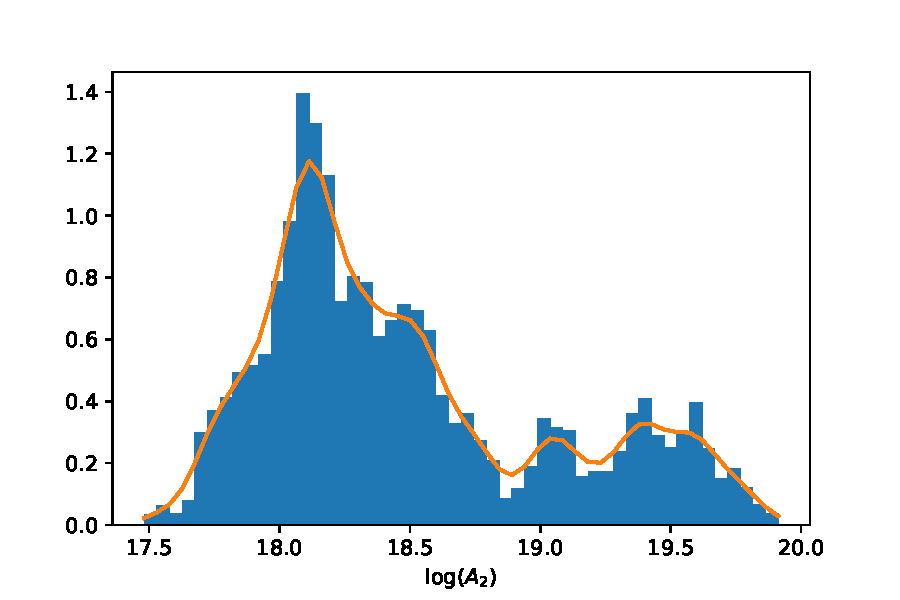
\includegraphics[width=\linewidth]{figures/bayesian/2_reactions/mass/hist_A2.pdf}
\caption{Histogram of $\tilde{A_2}$.}
\label{HistA2}
\end{subfigure}
\newline
\begin{subfigure}{0.5\textwidth}
\centering
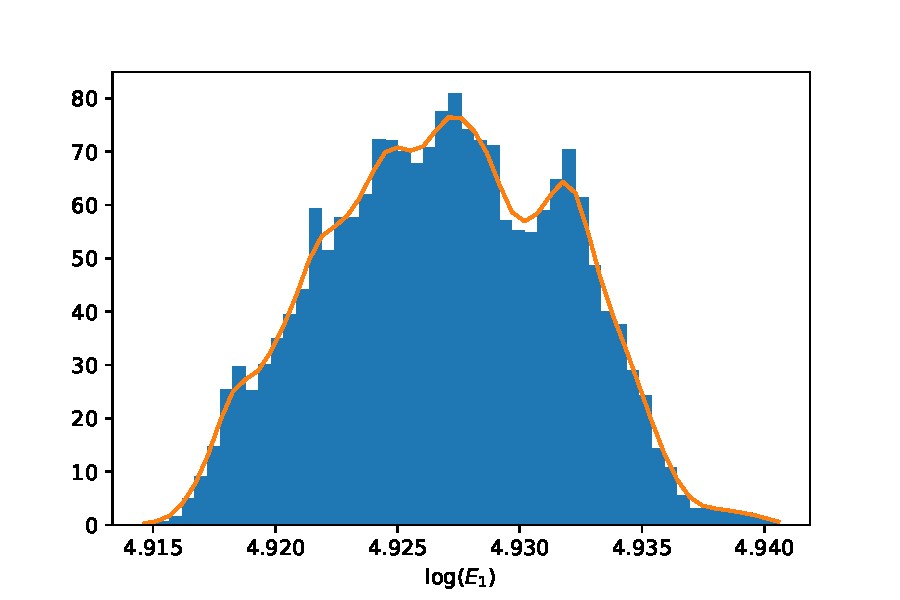
\includegraphics[width=\linewidth]{figures/bayesian/2_reactions/mass/hist_E1.pdf}
\caption{Histogram of $\tilde{E_1}$.}
\label{HistE1}
\end{subfigure}%
\begin{subfigure}{0.5\textwidth}
\centering
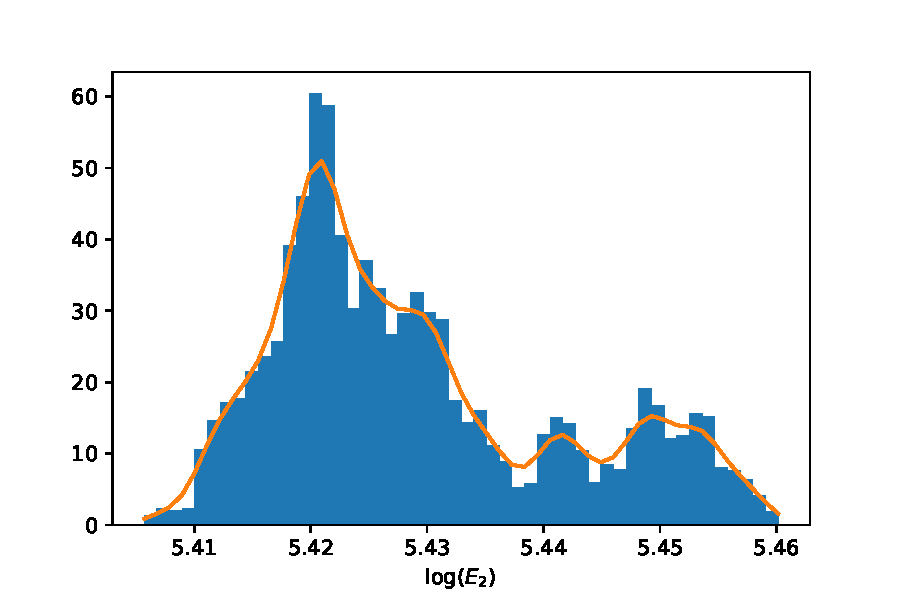
\includegraphics[width=\linewidth]{figures/bayesian/2_reactions/mass/hist_E2.pdf}
\caption{Histogram of $\tilde{E_2}$.}
\label{HistE2}
\end{subfigure}
\newline
\begin{subfigure}{0.5\textwidth}
\centering
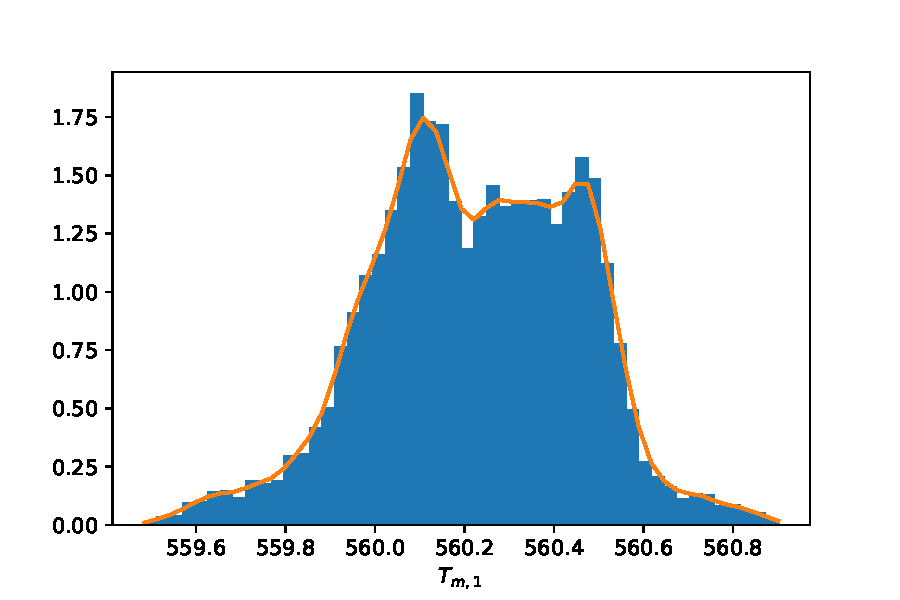
\includegraphics[width=\linewidth]{figures/bayesian/2_reactions/mass/hist_Tm1.pdf}
\caption{Histogram of $T_{m,1}$}
\label{HistTm1}
\end{subfigure}%
\begin{subfigure}{0.5\textwidth}
\centering
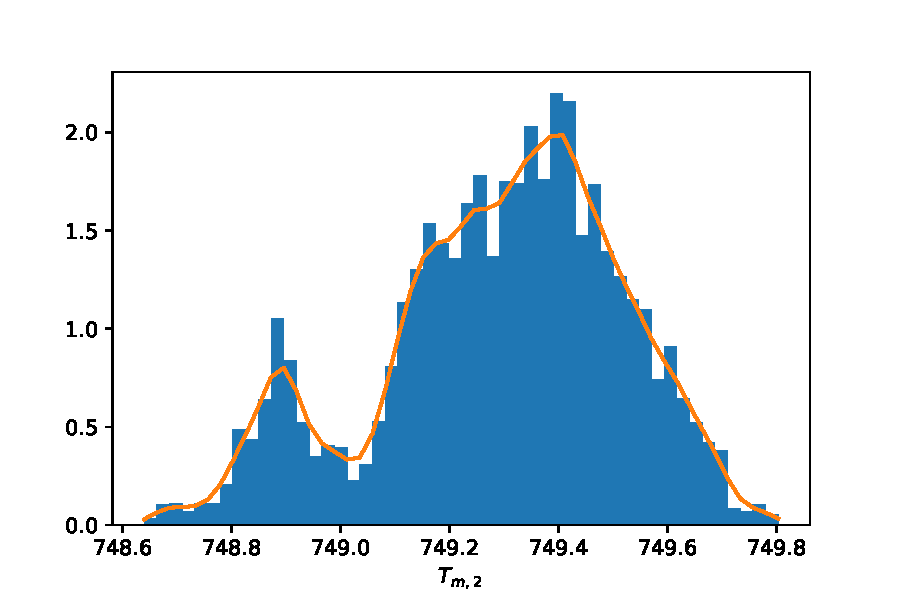
\includegraphics[width=\linewidth]{figures/bayesian/2_reactions/mass/hist_Tm2.pdf}
\caption{Histogram of $T_{m,2}$}
\label{HistTm2}
\end{subfigure}%
\newline
\begin{subfigure}{0.5\textwidth}
\centering
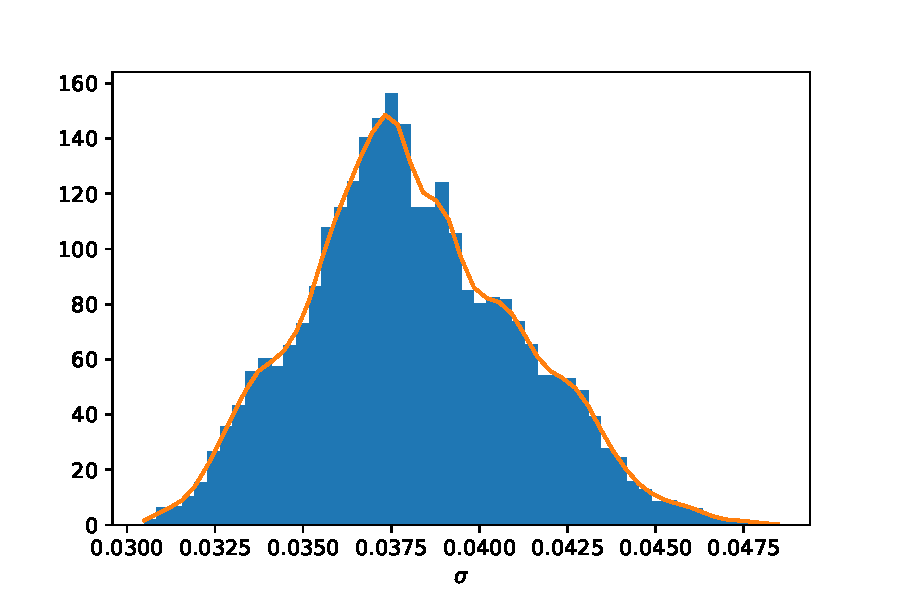
\includegraphics[width=\linewidth]{figures/bayesian/2_reactions/mass/hist_sigma.pdf}
\caption{Histogram of $\sigma$}
\label{Histsigma2}
\end{subfigure}%
\caption{Output from the Metropolis-Hastings for an experiment with two reactions.}
\label{fig:MH3}
\end{figure}

\begin{figure}[h!]
\centering
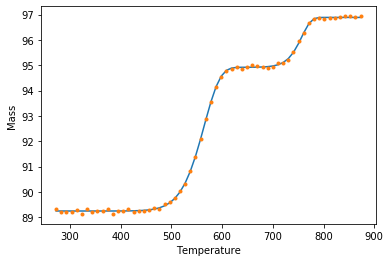
\includegraphics[scale=0.7]{figures/bayesian/2_reactions/mass/Example_FWC.png}
\caption{Example of a FWC change curve with two seperated equations.}
\label{fig:FWC_EX2}
\end{figure}

Figure \ref{fig:FWC_EX2}, plots an example of the FWC curve, generated using one of the sampled points and compares this to the the noisy data. This highlights an issue that may be arising from a lack of datapoints. There are minimal datapoints where the seond reaction is occurring, and this may contribute to why the sample obtained does not include the true parameters. Figure \ref{fig:FWC_EX2} clearly indicates that the sampled parameters still provide a good fit for the data.\\

This data is very simple, with well separated reactions. This indicates that our algorithm is useful to estimate these parameters for well seperated reactions. In the experimental data we use, the reactions are not well seperated. We simulate some new data using altered parameters. We change the parameters $T_{m,1}$ and $T_{m,2}$ such that, $T_{m,1}=620$ and $T_{m,2}=700$. Given these values are much closer, from the data itself it is harder to distinguish where the two peaks are. The non-overlapping uniform prior will not be useful in this scenario. Instead we consider a uniform prior over the region, $550<T_{m,1}<T_{m,2}<750$. This prior enforces our identifiability constraint, $T_{m,1}<T_{m,2}$, and bounds each value. It is possible to have other priors that fit these constraints, though we use this prior for its simplicity.\\

Conducting the inference we obtain the samples displayed in Figure \ref{fig:MH4}. In these samples we correctly obtain the true parameter values for each parameter. With the additional data points we do not have the issue before where the true parameter was outside our sampled values. We are able to successfully implement our algorithm to estimate the parameters with two reactions. It is reasonable to expect that we can apply this algorithm to include additional reactions. There is limitations that the reactions will have to be seperated in such a way that we can impose useful prior information.

\begin{figure}[h!]
\centering
\begin{subfigure}{0.5\textwidth}
\centering
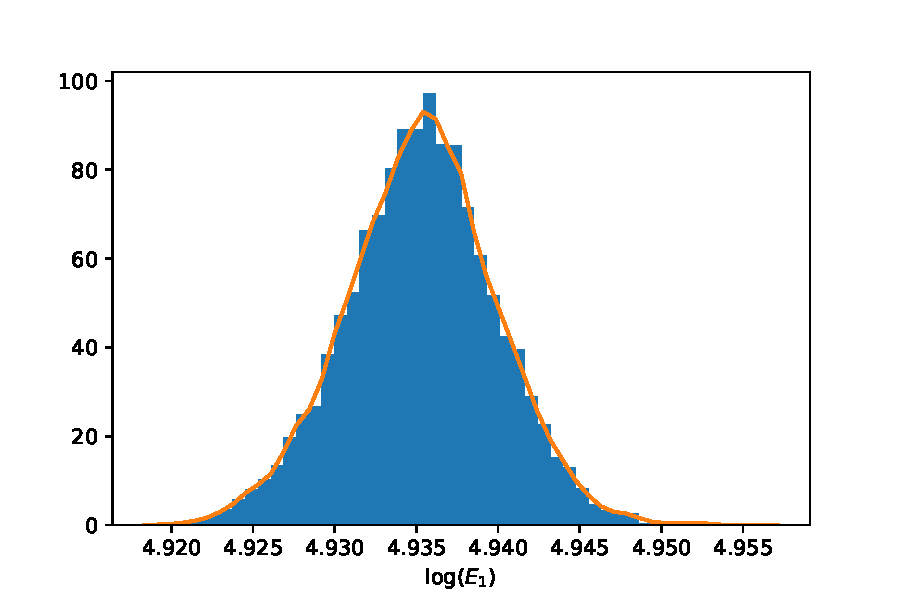
\includegraphics[width=\linewidth]{figures/bayesian/2_reactions/mass_close/hist_E1.pdf}
\caption{Histogram of $\tilde{E_1}$.}
\label{HistE12}
\end{subfigure}%
\begin{subfigure}{0.5\textwidth}
\centering
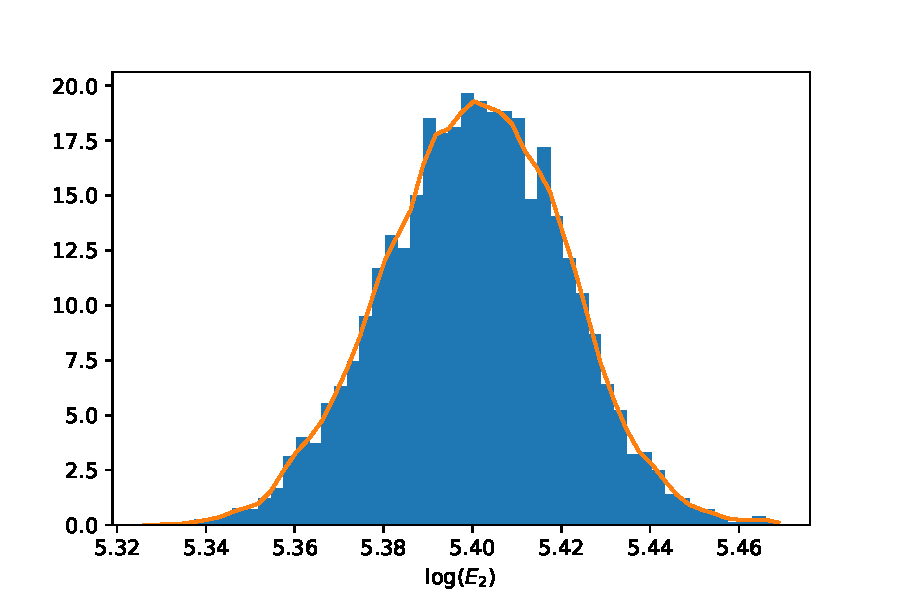
\includegraphics[width=\linewidth]{figures/bayesian/2_reactions/mass_close/hist_E2.pdf}
\caption{Histogram of $\tilde{E_2}$.}
\label{HistE22}
\end{subfigure}
\newline
\begin{subfigure}{0.5\textwidth}
\centering
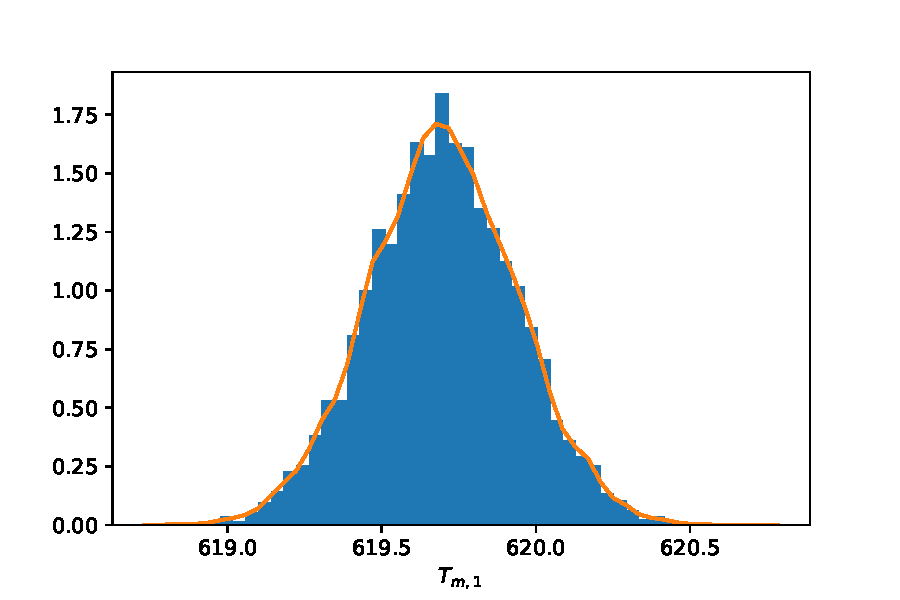
\includegraphics[width=\linewidth]{figures/bayesian/2_reactions/mass_close/hist_Tm1.pdf}
\caption{Histogram of $T_{m,1}$}
\label{HistTm12}
\end{subfigure}%
\begin{subfigure}{0.5\textwidth}
\centering
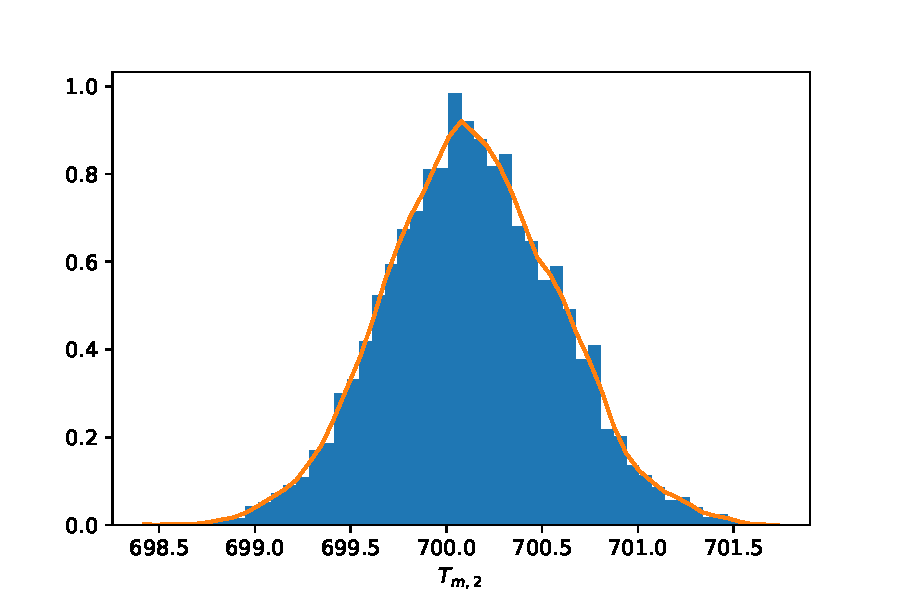
\includegraphics[width=\linewidth]{figures/bayesian/2_reactions/mass_close/hist_Tm2.pdf}
\caption{Histogram of $T_{m,2}$}
\label{HistTm22}
\end{subfigure}%
\newline
\begin{subfigure}{0.5\textwidth}
\centering
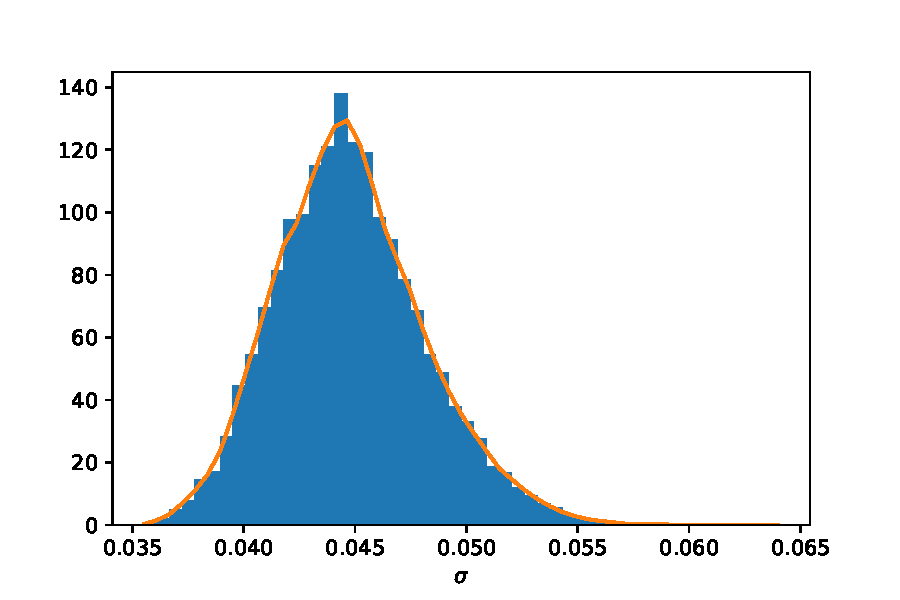
\includegraphics[width=\linewidth]{figures/bayesian/2_reactions/mass_close/hist_sigma.pdf}
\caption{Histogram of $\sigma$}
\label{Histsigma22}
\end{subfigure}%
\caption{Output from the Metropolis-Hastings for an experiment with two reactions, close together.}
\label{fig:MH4}
\end{figure}


\subsubsection{Multi-Modality}
The algorithm that we are using is not always work without issues. We found that when using a different model, our posterior distribution identified different modes. We use the model,
\begin{align*}
\frac{dM_1}{dt}&=-M_1OA_1\exp\left(\frac{-E_1}{RT}\right), \\
\frac{dM_2}{dt}&=-M_2^3OA_2\exp\left(\frac{-E_2}{RT}\right), \\ 
\frac{dT}{dt}&=\alpha, %\label{TGA_system2_BI}.
\end{align*}
This model is for a third order Arrhenious reaction for the second reaction rather than a first order. In future work we may consider different models, though our current analysis focuses upon first order reactions. \\
When using higher order reactions Equation \ref{eqkis}, becomes,
\begin{equation}
A\exp\left(\frac{-E}{RT_m}\right)nM_m^{n-1}=\frac{E}{RT_m^2}\frac{dT}{dt}, \label{eqkis2}
\end{equation}
where $n$, is the reaction order and $M_m$ is the mass when the reaction rate is maximised. We cannot use this equation to propose new values of $A$, as the mass term $M_m$ is dependant upon the parameters $(A,E,T_m)$. This yields an implicitly defined function for $A$, which is unlikely to yield any significant gains in computation speed. We can still use the Equation \ref{eqkis} as a means to propose new $A$ values, though the $T_m$ parameter in this case will not have the same meaning. This still reduces some of the issues we found when using the parameters $(A,E)$, though the prior information is not as useful.\\

We produce a simulated sample using the same parameters specified in Table \ref{sim_paras}. These parameters use Equation \ref{eqkis} to relate the Pre-exponential factor to the Activation Energy, and temperature $T_m$. This simulated data is displayed in Figure \ref{fig:modal_sim}. We observe that the second reaction rate is not maximised at the $T_m$ value stated in Table \ref{sim_paras}. This also highlights some issues with identifiability of the two reactions. We can no longer define the order of the reactions using this $T_m$ parameter.
 
\begin{figure}[h!]
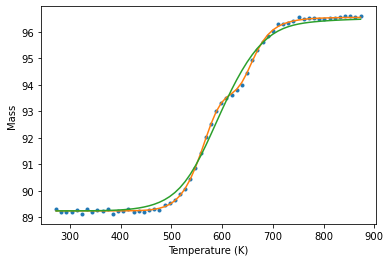
\includegraphics[scale=1]{figures/bayesian/2_reactions/TGA_comparison.png}
\caption{This figure needs to be updated.}
\label{fig:modal_sim}
\end{figure}
%
%After running the MCMC algorithm we observed that it does not always converge. Figure \ref{comparison} depicts the estimated mass of the sample for different sampled parameters. We observe that in some cases, the chains appear to be blurring the reactions together. It appears as though the MCMC algorithm is sampling around a local optimum value rather than the true optimal value.\\

We examine the bahaviour of the four chains as they move through the parameter sapce. Figure \ref{fig:walks} indicates that the value that the mode each chain samples around is dependant upon the initial proposal for the sampling algorithm. We observe two chains (red and orange) sample the true parameters in our model, whilst the other chains sample a much larger region. \\

\begin{figure}[h!]
\centering
\begin{subfigure}{.5\textwidth}
  \centering
  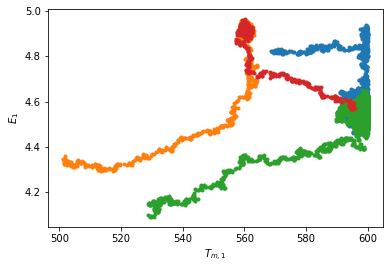
\includegraphics[width=\linewidth]{figures/bayesian/2_reactions/E1vsTm1.png}
  \caption{Random walks for the first reaction.}
  \label{fig:subwalk1}
\end{subfigure}%
\begin{subfigure}{.5\textwidth}
  \centering
  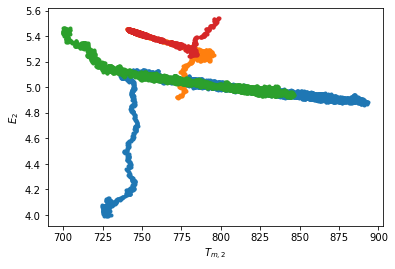
\includegraphics[width=\linewidth]{figures/bayesian/2_reactions/E2vsTm2.png}
  \caption{Random walks for the second reaction.}
  \label{fig:subwalk2}
\end{subfigure}%
\caption{Random walks for the maximal temperature and activation energy for the two reactions in a simulated system.}
\label{fig:walks}
\end{figure}

We claimed earlier that by proposing new values of $T_m$, we are still able to eliminate some of the issues with proposing the parameters,$(A,E)$. Figure \ref{fig:modal_sample} indicates that the sample from the chains that converged around the true parameters are uncorrelated. This indicates that although the parameter $T_m$ has lost its physical interpretation, the parameters $(A,E)$ are still near correlated along the cruve in \ref{eqkis}.\\

\begin{figure}[h!]
\centering
\begin{subfigure}{.5\textwidth}
  \centering
  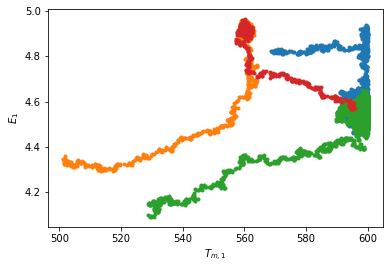
\includegraphics[width=\linewidth]{figures/bayesian/2_reactions/E1vsTm1.png}
  \caption{Random walks for the first reaction.}
  \label{fig:subwalk1}
\end{subfigure}%
\begin{subfigure}{.5\textwidth}
  \centering
  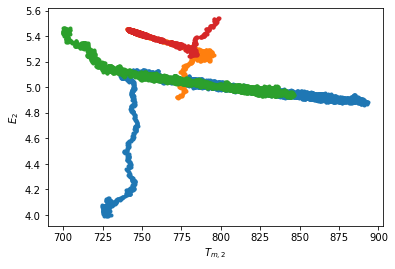
\includegraphics[width=\linewidth]{figures/bayesian/2_reactions/E2vsTm2.png}
  \caption{Random walks for the second reaction.}
  \label{fig:subwalk2}
\end{subfigure}%
\caption{Samples of the converged chain for the maximal temperature and activation energy for the two reactions in a simulated system.}
\label{fig:modal_sample}
\end{figure}

\begin{figure}[h!]
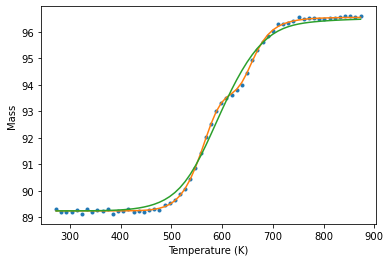
\includegraphics[scale=1]{figures/bayesian/2_reactions/TGA_comparison.png}
\caption{Comparison of two sampled parameter values for the two reaction case.}
\label{comparison}
\end{figure}

Figure \ref{comparison} plots example FWC curves within each mode. We see that mode 1 is able to approximate the data well whilst mode 2, seems to approximate the two reactions by a single reaction. This could potentially arise from the fact we are not using good information about the $T_m$ parameter. Implementing this in the way we have, could disrupt the algorithms ability to identify the reaction order and this results in this mode occuring. The key takeaway frm this is when we consider the experimental data, this issue may occur. The multi-modality is something we need to take into consideration.

\subsection{DSC}
With the issues of multi-modality we opt to use more of the experimental data. We include the addition of the DSC data into our simulations. The contribtion of each reaction to the DSC data is proportional to the reaction rate. By adding the DSC data, we are effectively adding information about the gradients of the FWC into our algorithm. This will ensure that what we observed in Figure \ref{comparison}, where the reactions combine, have a significantly lower likelihood. The adjusted algorithm is displayed in Algorithm \ref{Alg:MH_DSC}. It is important to note that the DSC data is calculated based off the mass of each substance from our solution vector.\\

Utilising the DSC data introduce s two new variables into the equation, $Q_1$ and $Q_2$. These denote the heat given by the reaction. We deal with the parameters in two ways. We can pre-assign the parameter values, or we can estimate these parameters through the MCMC algorithm. The results presented in Figure \ref{fig:DSC_4hist} use preassigned values. For the experimental data we estimate these parameters as they can be used to provide a better fit for the data. If there are multiple reactions occurring that mimic a single reaction. Estimating the heat of reaction parameters allows us to capture this information and characterise the heat in terms of a single reaction. This provides more valuable information when translating the theory across to the stockpiles where the temperature at each point of the pile is the key piece of information we are interested in.\\
We also have to consider the error for each of the mass and DSC data. We want to ensure that our algorithm isn't favouring one set of data over the other. We address this in our algorithm by setting the noise parameters so that the relative variances scale. The alternative is to have separate noise parameters to estimate. We have opted to include separate noise parameters, and then use the prior to force the variances to scale in some degree.\\

\begin{algorithm}[H]
\SetAlgoLined
\KwResult{}
 Initialise $\theta_0$ by sampling from the prior\;
 \For{$t=0:$sample\_size}{
  Sample $\theta ^*~ \sim ~ Q(\theta^*|\theta)$ \;
  Evaluate $\textbf{F}_\tau(\theta^*)$ \# solve differential equation\;
  Evaluate $\textbf{D}_\tau(\theta^*)$ \# calculate the DSC\;
  Set $\alpha = \frac{P(\textbf{y}|\theta^*)Q(\theta_{t-1}|\theta^*)P(\theta^*)}{P(\textbf{y}|\theta)Q(\theta^*|\theta_{t-1})P(\theta_{t-1})}$\;
  Sample $b ~ \sim ~U(0,1)$\;
  \eIf{$\alpha>b$}{
   Set $\theta_t=\theta^*$} {
   Set $\theta_t=\theta_{t-1}$
   }
 }
 \caption{Metropolis Hastings Algorithm for determining the posterior distribution with FWC and DSC data.}
 \label{Alg:MH_DSC}
\end{algorithm}

With this algorithm we now consider two cases; Fixed heat parameters, where we prescribe the values of $Q_1$ and $Q_2$, and our Inferred Parameters, where we conduct inference on the parameters $Q_1$ and $Q_2$.  
\subsubsection{Fixed Heat Parameters}
The first case is where we consider fixed heat parameters. This is a simple case where we can examine the effects of the addition of the DSC data without increasing the dimension of our problem. In a practical application we may not be able to prescribe these heat parameters and this limits the practical implementation of this method. Figure \ref{fig:DSC_4hist} displays the posterior distributions obtained from the simulated data. When we compare that to the data posterior samples in Figure \ref{fig:MH4}, then we observe that the histograms are much narrower. The samples in Figure \ref{fig:DSC_4hist} still contain the true values as well. With adding the DSC data into the simulations we have decreased the uncertainty in the posterior distributions.\\
%
\begin{figure}[h!]
\centering
\begin{subfigure}{.5\textwidth}
  \centering
  \includegraphics[width=\linewidth]{figures/bayesian/SIM/hist_E1.pdf}  \caption{Distribution of $\log E_1$.}
  \label{fig:subhistE1}
\end{subfigure}%
\begin{subfigure}{.5\textwidth}
  \centering
  \includegraphics[width=\linewidth]{figures/bayesian/SIM/hist_E2.pdf}
  \caption{Distribution of $\log E_2$.}
  \label{fig:subhistE2}
\end{subfigure}
\newline
\begin{subfigure}{.5\textwidth}
  \centering
  \includegraphics[width=\linewidth]{figures/bayesian/SIM/hist_Tm1.pdf}
  \caption{Distribution of $T_{m,1}$.}
  \label{fig:subhistTm1}
\end{subfigure}%
\begin{subfigure}{.5\textwidth}
  \centering
  \includegraphics[width=\linewidth]{figures/bayesian/SIM/hist_Tm2.pdf}
  \caption{Distribution of $T_{m,2}$.}
  \label{fig:subhistTm2}
\end{subfigure}
\newline
\begin{subfigure}{.5\textwidth}
  \centering
  \includegraphics[width=\linewidth]{figures/bayesian/SIM/hist_sigma.pdf}
  \caption{Distribution of $\sigma$.}
  \label{fig:subhistTm1}
\end{subfigure}%
%\begin{subfigure}{.5\textwidth}
%  \centering
%  \includegraphics[width=\linewidth]{figures/bayesian/SIM/hist_sigmaD.pdf}
%  \caption{Distribution of $\sigma_D$.}
%  \label{fig:subhistTm2}
%\end{subfigure}
    \caption{Distributions of the estimated parameters.}%
    \label{fig:DSC_4hist}%s}
\end{figure}%

\subsubsection{Inferred Parameter}
The alternative method for including these heat parameters is to conduct inference on them. This setting is more useful for practical problems where these parameters are unknown. As mention before that introducing new parameters into the inference increases the dimensionality of the problem and could lead to more multi-modal behaviour. The samples from the posterior distribution are displayed in Figure \ref{fig:DSC_8hist}

\begin{figure}[h!]
\centering
\begin{subfigure}{.5\textwidth}
  \centering
  \includegraphics[width=\linewidth]{figures/bayesian/SIM_Q/hist_E1.pdf}  \caption{Distribution of $\log E_1$.}
  \label{fig:subhistE1}
\end{subfigure}%
\begin{subfigure}{.5\textwidth}
  \centering
  \includegraphics[width=\linewidth]{figures/bayesian/SIM_Q/hist_E2.pdf}
  \caption{Distribution of $\log E_2$.}
  \label{fig:subhistE2}
\end{subfigure}
\newline
\begin{subfigure}{.5\textwidth}
  \centering
  \includegraphics[width=\linewidth]{figures/bayesian/SIM_Q/hist_Tm1.pdf}
  \caption{Distribution of $T_{m,1}$.}
  \label{fig:subhistTm1}
\end{subfigure}%
\begin{subfigure}{.5\textwidth}
  \centering
  \includegraphics[width=\linewidth]{figures/bayesian/SIM_Q/hist_Tm2.pdf}
  \caption{Distribution of $T_{m,2}$.}
  \label{fig:subhistTm2}
\end{subfigure}
\newline
\begin{subfigure}{.5\textwidth}
  \centering
  \includegraphics[width=\linewidth]{figures/bayesian/SIM_Q/hist_Q1.pdf}
  \caption{Distribution of $Q_{1}$.}
  \label{fig:subhistTm1}
\end{subfigure}%
\begin{subfigure}{.5\textwidth}
  \centering
  \includegraphics[width=\linewidth]{figures/bayesian/SIM_Q/hist_Q2.pdf}
  \caption{Distribution of $Q_{2}$.}
  \label{fig:subhistTm2}
\end{subfigure}
\newline
\begin{subfigure}{.5\textwidth}
  \centering
  \includegraphics[width=\linewidth]{figures/bayesian/SIM_Q/hist_sigma.pdf}
  \caption{Distribution of $\sigma$.}
  \label{fig:subhistTm1}
\end{subfigure}%
\begin{subfigure}{.5\textwidth}
  \centering
  \includegraphics[width=\linewidth]{figures/bayesian/SIM_Q/hist_sigmaD.pdf}
  \caption{Distribution of $\sigma_D$.}
  \label{fig:subhistTm2}
\end{subfigure}
    \caption{Distributions of the estimated parameters.}%
    \label{fig:DSC_8hist}%s}
\end{figure}%

When we compare the histograms in Figure \ref{fig:DSC_8hist} to those in Figure \ref{fig:DSC_4hist}, then we observe that the variance of the posterior distributions is much greater when we infer the heat parameters. This is not a surprising result as we are adding in more unknowns into the model. Figure \ref{fig:DSC_8hist} also indicates that we have successfully captured the true parameters within our posterior distrbutions. (Currently I have used the old values in the script and didn't update them so they are different).



\section{Application to Experimental Data}
Now that we have established the algorithm is able to infer information about our parameters in our simulated examples we can apply this to experimental data. The experimental data is more complex and there is also the case where we can have model misspecification. We persist with the model,
\begin{align}
\frac{dM_1}{dt}&=M_1A_1\exp\left(\frac{-E_1}{RT}\right),\\
\frac{dM_2}{dt}&=M_2A_2\exp\left(\frac{-E_2}{RT}\right),\\
\frac{dT}{dt}&=\alpha,\\
\frac{dM_t}{dt}&=w_{c,1}M_1A_1\exp\left(\frac{-E_1}{RT}\right)+w_{c,2}M_2A_2\exp\left(\frac{-E_2}{RT}\right), \\
H&=Q_1M_1A_1\exp\left(\frac{-E_1}{RT}\right)+Q_2M_2A_2\exp\left(\frac{-E_2}{RT}\right),\\
\end{align}
that we derived the respective parts for in Section \ref{SEC:TGA}. This first order Arrhenious equation model will also link into our large stockpile models and thus it is imperative that we conduct inference on these parameters. The experimental data is obtained from the work done by Longbottom et al \cite{Ray19} and displayed in Figure \ref{fig:EXP_data}.\\ 

\begin{figure}[h!]
\centering
\begin{subfigure}{.5\textwidth}
  \centering
  \includegraphics[width=\linewidth]{figures/TGA_exp.jpg}  
  \caption{Fractional weight change curve.}
  \label{fig:exp_fwc}
\end{subfigure}%
\begin{subfigure}{.5\textwidth}
  \centering
  \includegraphics[width=\linewidth]{figures/DSC_exp.jpg}
  \caption{Differential Scanning Calorimetry data.}
  \label{fig:exp_DSC}
\end{subfigure}
\label{fig:EXP_data}
\caption{Experimental data on the Filter cake \cite{Ray19}.}
\end{figure} 

This data includes all the reactions that are occuring within the stockpile. If we were to use all of the data we would need at least 5 reactions, of which many are unlikely to be identified through experimentation. We focus our analysis on the critical region from $200^oC$ to $500^oC$. This region was identified by Longbottom et al. \cite{Ray19} as the region where the reaction that are the primary drivers of selfheating are occuring. The restricted data is displayed in Figure \ref{fig:Res_data}, for clarity.\\

\begin{figure}[h!]
\centering
\begin{subfigure}{.5\textwidth}
  \centering
  \includegraphics[width=\linewidth]{figures/FWC.png}  
  \caption{Restricted FWC curve.}
\end{subfigure}%
\begin{subfigure}{.5\textwidth}
  \centering
  \includegraphics[width=\linewidth]{figures/Dsc.png}
  \caption{Restricted DSC data.}
  \label{fig:res_DSC}
\end{subfigure}
\label{fig:Res_data}
\caption{Experimental data on the Filter cake restricted to the critical region \cite{Ray19}.}
\end{figure}

When we are applying the algorithm to experimental data it is important to consider the effect of the parameters we aren't conducting the inference on. The specific parameters of interest are the initial mass concentrations, denoted $M_{1,0}$ and $M_{2,0}$, and the weight change constants, $w_{c,1}$ and $w_{c,2}$. We determine the weight change constants by prescribing the reaction scheme, 
\begin{align*}
3\text{Fe}+2\text{O}_2 &\rightarrow \text{Fe}_3\text{O}_4, \\
6\text{FeO}+\text{O}_2 &\rightarrow 2\text{Fe}_3\text{O}_4, \\
\end{align*}
stated in Section \ref{Sec:stockpile}. Using this reaction scheme we can determine the amount of mass that is added to the sample per gram of Iron and W\"ustite consumed. These weight change constants are stated in nomenclature.\\
The initial masses are more challenging. The filter cake is known to be highly heterogeneous and as a result the initial masses in the sample can vary from the measured values determined by Longbottom et al \cite{Ray19}. It is important to have accurate estimates for these parameters as they can introduce error into the model and the estimates of the reaction parameters can have an unkown bias. We control for this by ensuring that the simulated sample mass at the beginning and end of the critical region closely match the sample mass in the experiment. To calculate this we impose an assumption that there is negligible mass change from these reactions outside of this region. Under this assumption we also assume that the moistureless mass is the minimum sample mass. This results in the equation,
\begin{equation}
M_{1,0}w_{c,1}+M{2,0}w_{c,2}=M_{t,0}-M_{t,f}. \label{eq:constraint}
\end{equation} 
To determine the initial concentrations we minimise the distance, $d=\lvert \left(M_{1,0}-\tilde{M_1},M_{2,0}-\tilde{M_2}\right \rvert$, subject to the constraint \ref{eq:constraint}, where $ \tilde{M_1}$ and $\tilde{M_2}$ are the masses calculated using the percentage of moistureless mass determined by Longbottom et al \cite{Ray19}. We calculate the proportion of moistureless mass of Iron, $M_1$, and W\"ustite, $M_2$, to be 14.95\% and 29.42\%. Both of these values are less than those measured by Longbottom et al \cite{Ray19}, 16.4\% and 29.8\%. Our assumptions influence this as, if the reaction is continuting before and after this window we are investigating, then our method would understimate the these percentages. Due to the difficulty in obtaining precise measurements for these quantities, then we persist with this approximation method as it is deemed sufficient enough.\\
With all these assumptions we can conduct our inference on the data. The samples obtained through our algorithm are displayed in Figure \ref{fig:EXP_histograms}. These Histograms appear nicely behaved and indicate a slightly greater spread of values than what we experience in the simulated studies. This is to be expected as we expect that some model misspesification can occur. The spread of these histograms are quite similar to those achieved when we consider two reactions close together only using the FWC data presented in Figure \ref{fig:MH4}. The parameter with the greatest uncertainty in comparison to the results with two reactions, is the temperature at which the first reaction is maximised, $T_{m,1}$. 

\begin{figure}[h!]
\centering
\begin{subfigure}{.5\textwidth}
  \centering
  \includegraphics[width=\linewidth]{figures/bayesian/EXP_Q/hist_E1.pdf}  \caption{Distribution of $\log E_1$.}
  \label{fig:subhistE1}
\end{subfigure}%
\begin{subfigure}{.5\textwidth}
  \centering
  \includegraphics[width=\linewidth]{figures/bayesian/EXP_Q/hist_E2.pdf}
  \caption{Distribution of $\log E_2$.}
  \label{fig:subhistE2}
\end{subfigure}
\newline
\begin{subfigure}{.5\textwidth}
  \centering
  \includegraphics[width=\linewidth]{figures/bayesian/EXP_Q/hist_Tm1.pdf}
  \caption{Distribution of $T_{m,1}$.}
  \label{fig:subhistTm1}
\end{subfigure}%
\begin{subfigure}{.5\textwidth}
  \centering
  \includegraphics[width=\linewidth]{figures/bayesian/EXP_Q/hist_Tm2.pdf}
  \caption{Distribution of $T_{m,2}$.}
  \label{fig:subhistTm2}
\end{subfigure}
\newline
\begin{subfigure}{.5\textwidth}
  \centering
  \includegraphics[width=\linewidth]{figures/bayesian/EXP_Q/hist_Q1.pdf}
  \caption{Distribution of $Q_{1}$.}
  \label{fig:subhistTm1}
\end{subfigure}%
\begin{subfigure}{.5\textwidth}
  \centering
  \includegraphics[width=\linewidth]{figures/bayesian/EXP_Q/hist_Q2.pdf}
  \caption{Distribution of $Q_{2}$.}
  \label{fig:subhistTm2}
\end{subfigure}
\newline
\begin{subfigure}{.5\textwidth}
  \centering
  \includegraphics[width=\linewidth]{figures/bayesian/EXP_Q/hist_sigma.pdf}
  \caption{Distribution of $\sigma$.}
  \label{fig:subhistsigma}
\end{subfigure}%
\begin{subfigure}{.5\textwidth}
  \centering
  \includegraphics[width=\linewidth]{figures/bayesian/EXP_Q/hist_sigmaD.pdf}
  \caption{Distribution of $\sigma_D$.}
  \label{fig:subhistsigmad}
\end{subfigure}
    \caption{Distributions of the estimated parameters from the experimental data.}%
    \label{fig:EXP_histograms}%s}
\end{figure}%



When we apply this algorithm to experimental data it is important to carefully examine the convergence of each of the four chains in our algorithm. These investigatons can be carried out with the our simulated data, though given we know the true values we an get an appreciable idea of whether they have converged using the sample. The associated plots for the simulated data are contained in Appendix \ref{App:2_traces}. We investigate the samples by first inspecting the traceplots. We expect that the four chains should be well mixed. We also want to observe chains that have a low autocorrelation, and this can be observed qualitatively by observing the chains but can also be obsrved in a quantitative manner using the effective sample size (ESS).


\begin{figure}[h!]
\centering
\begin{subfigure}{.5\textwidth}
  \centering
  \includegraphics[width=\linewidth]{figures/bayesian/EXP_Q/trace_plot_E1.pdf}  \caption{Trace plot of $\log E_1$.}
  \label{fig:subtpE1}
\end{subfigure}%
\begin{subfigure}{.5\textwidth}
  \centering
  \includegraphics[width=\linewidth]{figures/bayesian/EXP_Q/trace_plot_E2.pdf}
  \caption{Trace plot of $\log E_2$.}
  \label{fig:subtpE2}
\end{subfigure}
\newline
\begin{subfigure}{.5\textwidth}
  \centering
  \includegraphics[width=\linewidth]{figures/bayesian/EXP_Q/trace_plot_Tm1.pdf}
  \caption{Trace plot of $T_{m,1}$.}
  \label{fig:subtpTm1}
\end{subfigure}%
\begin{subfigure}{.5\textwidth}
  \centering
  \includegraphics[width=\linewidth]{figures/bayesian/EXP_Q/trace_plot_Tm2.pdf}
  \caption{Trace plot of $T_{m,2}$.}
  \label{fig:subtpTm2}
\end{subfigure}
\newline
\begin{subfigure}{.5\textwidth}
  \centering
  \includegraphics[width=\linewidth]{figures/bayesian/EXP_Q/trace_plot_Q1.pdf}
  \caption{Trace plot of $Q_{1}$.}
  \label{fig:subtpTm1}
\end{subfigure}%
\begin{subfigure}{.5\textwidth}
  \centering
  \includegraphics[width=\linewidth]{figures/bayesian/EXP_Q/trace_plot_Q2.pdf}
  \caption{Trace plot of $Q_{2}$.}
  \label{fig:subtpTm2}
\end{subfigure}
\newline
\begin{subfigure}{.5\textwidth}
  \centering
  \includegraphics[width=\linewidth]{figures/bayesian/EXP_Q/trace_plot_sigma.pdf}
  \caption{Trace plot of $\sigma$.}
  \label{fig:subtpsigma}
\end{subfigure}%
\begin{subfigure}{.5\textwidth}
  \centering
  \includegraphics[width=\linewidth]{figures/bayesian/EXP_Q/trace_plot_sigmaD.pdf}
  \caption{Trace plot of $\sigma_D$.}
  \label{fig:subtpsigmad}
\end{subfigure}
    \caption{Trace plots of the estimated parameters from the experimental data.}%
    \label{fig:EXP_TP}%
\end{figure}%

Figure \ref{fig:EXP_TP} displays the trace plots for each of the inferred parameters and seems to indicate that the chains do converge. We observe the initil period where we have a lower acceptance rate. We can accept this as it will allow the algorithm to explore greater regions of the parameter space. By having a variable proposal distribution, in the initial stages of the algorithm we can have a lower acceptance rate as we attempt to explore more of the parameter space. Once the Markov Chains begin to converge onto the posterior distribution we adjust the proposal so that we can sample this distribution more efficiently. Figure \ref{fig:EXP_TP} shows that by using the four chains we have been able to explore different areas of the parameter space.

\begin{figure}[h!]
\centering
\begin{subfigure}{.5\textwidth}
  \centering
  \includegraphics[width=\linewidth]{figures/bayesian/EXP_Q/FWC.pdf}  
  \caption{Fractional weight change curve.}
  \label{fig:exp_fwc_comp}
\end{subfigure}%
\begin{subfigure}{.5\textwidth}
  \centering
  \includegraphics[width=\linewidth]{figures/bayesian/EXP_Q/DSC.pdf}
  \caption{Differential Scanning Calorimetry data.}
  \label{fig:exp_DSC_comp}
\end{subfigure}
\label{fig:EXP_data_comp}
\caption{Experimental data on the Filter cake \cite{Ray19}, compared to the posterior sampled values.}
\end{figure}

\begin{figure}[h!]
\centering
\begin{subfigure}{\textwidth}
  \centering
  \includegraphics[width=\linewidth]{figures/bayesian/EXP_Q/trace_plot_E1_burned.pdf} 
  \caption{Trace plot of $\log E_1$.}
  \label{fig:subtpburnE1}
\end{subfigure}%
\newline
\begin{subfigure}{\textwidth}
  \centering
  \includegraphics[width=\linewidth]{figures/bayesian/EXP_Q/trace_plot_E2_burned.pdf}
  \caption{Trace plot of $\log E_2$.}
  \label{fig:subtpburnE2}
\end{subfigure}
\newline
\begin{subfigure}{\textwidth}
  \centering
  \includegraphics[width=\linewidth]{figures/bayesian/EXP_Q/trace_plot_Tm1_burned.pdf}
  \caption{Trace plot of $T_{m,1}$.}
  \label{fig:subtpburnTm1}
\end{subfigure}%
\newline
\begin{subfigure}{\textwidth}
  \centering
  \includegraphics[width=\linewidth]{figures/bayesian/EXP_Q/trace_plot_Tm2_burned.pdf}
  \caption{Trace plot of $T_{m,2}$.}
  \label{fig:subtpburnTm2}
\end{subfigure}
\newline
\begin{subfigure}{\textwidth}
  \centering
  \includegraphics[width=\linewidth]{figures/bayesian/EXP_Q/trace_plot_Q1_burned.pdf}
  \caption{Trace plot of $Q_{1}$.}
  \label{fig:subtpburnTm1}
\end{subfigure}%
\newline
\begin{subfigure}{\textwidth}
  \centering
  \includegraphics[width=\linewidth]{figures/bayesian/EXP_Q/trace_plot_Q2_burned.pdf}
  \caption{Trace plot of $Q_{2}$.}
  \label{fig:subtpburnTm2}
\end{subfigure}
\newline
\begin{subfigure}{\textwidth}
  \centering
  \includegraphics[width=\linewidth]{figures/bayesian/EXP_Q/trace_plot_sigma_burned.pdf}
  \caption{Trace plot of $\sigma$.}
  \label{fig:subtpburnsigma}
\end{subfigure}%
\newline
\begin{subfigure}{\textwidth}
  \centering
  \includegraphics[width=\linewidth]{figures/bayesian/EXP_Q/trace_plot_sigmaD_burned.pdf}
  \caption{Trace plot of $\sigma_D$.}
  \label{fig:subburnsigmad}
\end{subfigure}
    \caption{Trace plots of the estimated parameters from the experimental data.}%
    \label{fig:EXP_TP_burned}%s}
\end{figure}% 

Figure \ref{fig:EXP_TP_burned} displays the trace plots after discarding the burn in period. In this figure we observe that the chains are mixing and are not getting stuck on a set of parameters. This indicates that the chains have converged and are effectively sampling the posterior distribution. These traceplots indicate that the chains have converged to the posterior distribution but it remains to be shown how reasonable this distribution is at following the experimental data. As we observed in Section \ref{Sec:1R_EXP}, that a one reaction model didn't sufficiently explain the data, and resulted in large variances in the posterior distribution. Figure \ref{fig:EXP_histograms} indicates that this may not be the case with our two reaction model. It is still useful to compare the experimental data.\\

Figure \ref{fig:EXP_data_comp} compares the simulated FWC and DSC data using 10 randomly sampled points from the posterior distribution. This figure indicates that the fit for the DSC data matches up well though we observe some issues with the weight change data. For the purposes of examining the heat generation within the stockpile it is more important that we approximate the DSC data as this directly relates to the heat generation from the reactions. We also observe that these 10 curves are clumped together providing further evidence of the Markov Chains converging.


    \chapter{Sequential Monte Carlo Sampling}
In the previous chapter we utilised a Metropolis-Hastings in order to sample from the posterior distribution of our parameters. These posteriors are dependant upon the observations of a single experiment. In practice these experiments are often repeated and can be carried out under different heating rates. To make use of this additional information then we could just add this to our original data and implement an MCMC algorithm for more data. This approach would be computationally costly and could present other issues arising from various modes appearing. Instead the approach that we use is through Importance Sampling (IS) and Sequential Monte Carlo (SMC).\\

\section{Importance Sampling}
Importance sampling is a resampling technique, where given a sample $\textbf{X}$, then for each point $\textbf{x}$ in our sample a weight $w$ is calculated. These weights are calculated through the liklihood function with respect to the second reaction  
    \chapter{Non-Dimesional Analysis}
One of the ways we can analyse the stockpile model,
\begin{equation}
\rho c \frac{\partial T}{\partial t}=\nabla \cdot \left(k\nabla T\right) +Q(T), \label{base2}
\end{equation}
stated in section \ref{Sec:stockpile}, is through non-dimensional analysis. In this technique we scale the dimensional variables, $x$, $t$ and $T$ using the constants that appear in the equations. This analysis allows us to determine some of the general features of the stockpiles. This analysis has been used to determine a relationship for the critical length of a stockpile, dependant upon the reaction kinetics. Within this chapter we will analyse, through non-dimensional analysis the effects that periodic boundary condition can have on stockpile ignition and also the effects of a hotspot within the stockpile for subcritical stockpile.\\

Considering a one-dimensional stockpile, of length $L$, with a first order Arrhenious reaction rate, we can use the scalings,
\begin{align*}
x^*&=\frac{x}{L},\\
t^*&= \frac{\alpha}{L^2}t, \\
u&=\frac{E}{RT_a^2}\left(T-T_a\right),
\end{align*} 
to reduce the equation to the non-dimensioanal form,
\begin{equation}
\frac{\partial u}{\partial t^*}=\frac{\partial^2 u}{\partial {x^*}^2}+\delta\exp\left(\frac{u}{1+\varepsilon u}\right), \label{eq:non-dim}
\end{equation}
where,
where $\varepsilon=T_a R/E$ and $$\delta=L_y^2\frac{Q\rho A}{k}\exp\left(\frac{-E}{RT_a}\right)\frac{E}{R T_a^2}.$$ The parameter $\delta$ is the Frank-Kamanetskii (FK) parameter. Using the Dirichlet boundary condition, $T=Ta$, then we obtain the non-dimensional boundary condition $u=0$. The domain of our scaled equation is $x^*\in [0,1]$. With this formulation we often have $\varepsilon \ll 1$ so we consider $\varepsilon=0$. In this case we have a critical Frank-Kamanetskii parameter such that if $\delta>\delta_{\text{cr}}$ then the stockpile will ignite, and if $\delta<\delta_{\text{cr}} $ then the stockpile will not ignite and is considered subcritical.\\

We can extend this non-dimensionalisation to higher spatial dimensions. If we consider three dimensions, $(x,y,z)$, then by scaling everything by the height, $L_y$, then Equation \ref{base2}, becomes,
\begin{equation}
\frac{\partial u}{\partial t^*}=\frac{\partial^2 u}{\partial {x^*}^2}+\frac{\partial^2 u}{\partial {y^*}^2}+\frac{\partial^2 u}{\partial {z^*}^2}+\delta\exp\left(\frac{u}{1+\varepsilon u}\right),
\end{equation}
on the domain $[0,L_x/L_y]\times[0,1]\times[0,L_z/L_y]$. We scale each spatial dimension by the same length since we maintain the laplacian in the equation. In this case the results are still dependant upon the shape of the domain but generally we will consider nice shapes where the lengths have certain nice ratios. From here we drop the $*$ from the dimensionless variables.\\

We need to define what we mean by ignition. In the theoretical case with $\varepsilon=0$, there is a point where there are no stable steady state solutions, and heating continues indefinitely \cite{bowes}. We can then state that supercritical stockpiles are those that will continue heating indefinitely and subcritical are those that do not. This phenomena cannot be determined numerically as we are restricted to finite times and temperatures. This asks the questions how can we define ignition in a practical sense. Within our model there are two things to consider: How hot does the stockpile need to get to to categorise the stockpile as supercritical, and how much time do we allow for the stockpile to reach this state. The answers to these are going to depend on the context of the problem that is being addressed. \\

For our context we generally consider ignition times of approximately one year. For the purposes of our analysis we will consider ignition occouring when the maximum non-dimensional temperature exceeds 100, $u_{\text{max}}=100$. Using the parameters used in a paper we published \cite{Berry19}, this equates to a temperature of roughly $800^oC$. The parameters used here are very similar to those we use in this thesis and as such the critical temperature is roughly $800^oC$. If we were to use a point estimate of $E=10^4.637$ for the experimental data, this would correspond to a critical temperature of $1600^oC$ which would be excessive. This highlights the need for these considerations to be made when applying the non-dimensional results to physical problems. When performing Nonidimensional analysis of the equations we are able to deduce relationships between certain parameters. 


\section{Periodic Boundary Conditions}
In the stockpile literature the boundary conditions do not depend upon time. In practicality the large stockpiles are left outside and subject to seasonal and dirunal variations in the ambient temperature. We only consider seasonal temperature variations within the scope of this thesis. We model the seasonal temperature variations using a sine function. The boundary condition becomes,
\begin{equation}
T=T_a+T_o\sin\left(\frac{2\pi t}{\omega_Y}+\phi\right), \label{eq:PBC_D}
\end{equation}
where $T_a$ is the average ambient temperature variation, $T_o$ is the maximum temperature oscillation, $\omega_Y$ is the oscillation period which for seasonal temperature variations is one year, and $\phi$ is a phase shift. After non=dimensionalising the boundary contition we obtain,
\begin{equation}
u=u_o \sin\left(\frac{2\pi t}{\omega}+\phi \right),
\end{equation} 
where $u_o=\left(E/RT_a^2\right)T_o,$ and $\omega=\alpha \omega_Y/L_y^2.$ The phase shift parameter $\phi$ allows us to control when during the year the stockpiles are constructed. When $\phi=0$, this would be indicative of a stockpile constructed in spring, whilst at $\phi=\pi/2$, this would be during summer when the ambient temperature is at its maximum. This is a very simple way to model the oscillations which also allows us to examine the relationship and effect on stockpile ignition.\\

When we extend this to higher dimensions we don't have all sides exposed to the ambient air. The base of the stockpile requires a seperate condition. For simplicity we assume that no heat is exchanged at this boundary, that is $\partial T/\partial y =0$. When we have this condition we are able to reflect around the plane $y=0$, which means we can use results where the boundary has the same condition.
 
\subsection{Dirichlet Boundary Condition}
Initially we consider a simple dirichlet boundary condition for two specific stockpile geometries, $L_x=2L_y$ and $L_x=\infty$. For the case where $L_x=2L_y$, the reflective condition prescribed at the boundary $y=0$ means that we can instead solve the problem on the square with non-dimensional length 2. This solution restricted to the domain $(0,2)\times (0,1)$ will solve our equation. For the approximation $\varepsilon=0$ and Dirichlet boundary conditions, the critical value is $\delta_{cr}=1.7$ \cite{bowes}. For $L_x \gg L_y$ we approximate the model by a one-dimensional model without diffusion in the $x$ direction. For the approximation $\varepsilon=0$ and static boundary condition the critical value is $\delta_{cr}=0.88$ \cite{bowes}. The value obtained from our simulations, displayed in Table \ref{1ddelt} equals the value stated by Bowes \cite{bowes} to the given number of significant figures.\\ 
\begin{table}[h!]
\caption{The critical Frank-Kamenetskii parameter, $\delta_{cr}$, in a one dimensional stockpile for different cut-off times with $u_o=0.637$, $\omega=0.3$ and $\phi=0$ for the cases with oscillations.}
\centering
\begin{tabular}{|c|c|c|c|c|c|}
\hline
$\varepsilon$ & Oscillations &$t_f=0.3$& $t_f=1$ & $t_f=10$ & $t_f=100$ \\ \hline
0 & no & 3.701 & 1.582 & 0.899 & 0.877 \\ \hline
0 & yes & 3.428 & 1.537 & 0.895 & 0.875 \\ \hline
0.027 & no & 3.910 & 1.658 & 0.927 & 0.904 \\ \hline
0.027 & yes & 3.639 & 1.612 & 0.924 & 0.901 \\ \hline
\end{tabular}
\label{1ddelt}
\end{table}
Table \ref{1ddelt} suggests that for the larger cut-off times ($t_f=10,100$) the dynamic boundary condition does not have a significant influence on the critical FK parameter with a slight reduction observed, when the oscillations are added. However, there is a significant difference in the ignition times.
For the case where $\varepsilon=0$, $\delta=0.89$, the ignition times are $\tig=14.00$ and $\tig=12.04$, for the dynamic and static boundary conditions respectively. Similarly for $\varepsilon=0.027$, $\delta=0.92$ and the static boundary condition, $\tig=12.40$ whilst with the dynamic boundary condition, $\tig=11.67$. This indicates that for a given stockpile the ignition time is different once the dynamic boundary condition is applied. \\ 
\begin{table}[h!]
\caption{The critical FK parameter $\delta_{cr}$ for a two-dimensional rectangular domain with $u_o=0.637$, $\omega=0.3$ and $\phi=0$.}
\centering
\begin{tabular}{|c|c|c|c|c|}
\hline
$\varepsilon$ & Oscillations & $t_f=0.3$ & $t_f=1$ & $t_f=10$ \\ \hline
0 & no & 4.072 & 2.20 & 1.71  \\ \hline
0 & yes & 3.615 & 2.14 & 1.69  \\ \hline
0.027 & no & 4.294 & 2.3 & 1.76  \\ \hline
0.027 & yes & 3.843 & 2.23 & 1.75  \\ \hline
\end{tabular}
\label{2ddelt}
\end{table}  
In two dimensions, the effects of the dynamic boundary condition are more prominent than with the static boundary condition. For the $\varepsilon=0$ case, the oscillations cause stockpiles to ignite that are \textit{subcritical} when considering a static boundary condition. The one-dimensional stockpiles have a lower critical value so one would expect as we increase the length, $L_x$, of the two-dimensional stockpile with fixed height, $L_y$, then this will decrease the critical parameter. This relationship is displayed in Figure \ref{ratio}.
\begin{figure}[h!]
\centering
\includegraphics[scale=0.8]{figures/NDA/PBC/deltavslength_both.pdf} 
\caption{The critical FK variable $\delta$ for ignition to occur within a year, as the ratio of side length to height is increased with $\epsilon=0.027$ and $\phi=0$.}
\label{ratio}
\end{figure}
For the static boundary condition, the critical value of the FK parameter approaches that calculated for the one dimensional model. \\
So far our analysis has assumed the stockpiles are constructed at a specific time of year, specifically spring, $\phi=0$. By setting $t_f=0.3$, Figure \ref{phi} indicates which stockpiles will ignite within a year. Certain stockpiles constructed in spring will ignite whilst identical ones constructed in Autumn will not.\\ 
\begin{figure}[h!]
\centering
\includegraphics[scale=0.8]{figures/NDA/PBC/phaseshift.pdf} 
\caption{The effects of changing the stockpile construction time ($\phi$) on the critical FK parameter, $\delta$, for stockpile ignition within a year ($t_f=0.3$).}
\label{phi}
\end{figure}
\begin{figure}[h!]
\centering
\includegraphics[scale=0.8]{figures/NDA/PBC/phaseshift2.pdf} 
\caption{The effects of changing the initial construction time ($\phi$) on the value of the critical FK parameter, $\delta$, for a final time, $t_f=1$, corresponding to just over a three year period.}
\label{phi2}
\end{figure}
The final time is increased to $t_f=1$. The critical Frank-Kamanetskii parameter becomes less sensitive to the construction date. Another key observation is that when $t_f=1$ there are more starting points where the critical parameter is lower than the static boundary condition. Figure \ref{phi2} shows a shift in the oscillation peak towards $\phi=0$. \\
We now consider the ignition times as the FK parameter ($\delta$) is varied.
\begin{figure}[h!]
\centering
\includegraphics[scale=0.8]{figures/NDA/PBC/ignitontimes.pdf}
\caption{The ignition times as the Frank-Kamanetskii parameter, $\delta$, is varied.}
\label{ignition}
\end{figure} 
Figure \ref{ignition} compares the ignition times for the static boundary condition with the dynamic boundary condition. Stockpiles constructed in spring, $\phi=0$, are plotted along with stockpiles constructed half a year later, $\phi=\pi$. For the larger values of the FK parameter, there is a distinct difference between the ignition times in each case. For smaller values of the FK parameter the ignition times for stockpiles constructed later ($\phi=\pi$) are lower than those with the static boundary condition. This indicates that as we consider longer periods of time the dynamic boundary condition reduces the ignition times. This Figure suggests that there will exist some time such that, regardless of when the stockpile is built, the effect of the dynamic boundary condition will cause the stockpile to ignite earlier than is the case for the static boundary condition.\\

\subsection{Newtonian Cooling Boundary Conditions}
The alternative to using a dirichlet boundary condition is to apply a convective heat transfer condtion. We use the same boundary condition defined in section \ref{Sec:models:BC}, with the ambient temperature following the same oscillations in equation \ref{eq:PBC_D}.
 
\section{Hotspot Ignition}
One of the theories to induce ignition within large stockpiles is to take a portion of material from a supercritical stockpile and add this to a stockpile that is subcritical. From a theoretical basis, in the approximation $\varepsilon=0$, if the temperature within the stockpile is high enough, then the reaction can continue out of control and the stockpile can become supercritical even for FK parameters less than the critical parameter. Since this is a possibility we seek to identify some of the conditions that leads to ignition occurring.\\
We introduce the hotspot by changing the initial temperature distribution. Our initial considerations is a uniform initial condition equal to that of the ambient temperature, ie, $u=0$. We introduce the hotspot by changing the initial condition to,
\begin{equation}
u=u_h\left(H(x-l-w/2)-H(x-l+w/2)\right),
\end{equation} 
where $u_h$ is the dimensionless hotspot temperature, $l$ is the centre location of the hotspot and $w$ is the width of the hotspot, generally expressed in terms of the ratio of hotspot to stockpile size. This formulation allows us to control the location, size and Temperature of the hotspot. We can obtain the nondimensional temperature using the equation,
\begin{equation}
u_h=\frac{E}{RT_a^2}\left(T_h-T_a\right),
\end{equation} 
where $T_h$ is the temperature of the hotspot.

\subsection{One-Dimensional Stockpiles}
To begin our analysis on stockpiles we consider a one-dimensional pile. These piles are the simplest and most computationally efficient to solve. This allows us to examine the dependencies efficiently and then we can generalise these to higher dimension stockpiles. The first relationship we explore is for a fixed size hotspot, how hot does this hotspot need to be in order to cause a subcritical stockpile to ignite. Figure \ref{fig:hot:delta1} displays this relation and indicates what we would expect that as we decrease the Frank-Kamanetskii parameter then we require a hotter hotspot to cause ignition.\\

\begin{figure}[h!]
\centering
\includegraphics[width=\linewidth]{figures/NDA/Hotspot/delta1.pdf}  
\caption{The temperature required for subcritical stockpile to ignite.}
\label{fig:hot:delta1}
\end{figure} 

Figure \ref{fig:hot:delta1} uses a hotspot that is 10\% of the size of the stockpile and located on the edge. It is worth investigation what occurs when we change these parameters. Figure \ref{fig:hot:size_loc} displays these results. We find that the size of the hotspot has a significant impact on the critical temperature. Figure \ref{fig:hot:size} also indicates that if the whole stockpile is heated initially to a point equivilant to $40^oC$ with our parameters, then this would be enough to get the stockpile to ignite. The location of the hotspot within the stockpile does not have a large impact on the necessary hotspot temperature. We observe that hotspots near the boundary require a slightly higher temerature and attribute this to the cooling that is occuring at the boundary.\\

\begin{figure}[h!]
\centering
\begin{subfigure}{.5\textwidth}
  \centering
  \includegraphics[width=\linewidth]{figures/NDA/Hotspot/size1.pdf}  
  \caption{Hotspot temperature required for different size hotspots.}
  \label{fig:hot:size}
\end{subfigure}%
\begin{subfigure}{.5\textwidth}
  \centering
  \includegraphics[width=\linewidth]{figures/NDA/Hotspot/Location1.pdf}
  \caption{Hotspot temperature for different hotspot locations}
  \label{fig:hot:loc}
\end{subfigure}
\label{fig:hot:size_loc}
\caption{The critical temperatures needed for different hotspots in order to cause ignition of subcritical stockpiles.}
\end{figure}

In the previous section we determined that periodic boundary conditions had an impact on the the critical delta parameter. It would then be useful to know if this has an impact on the critical hotspot temperature required for ignition. Figure \ref{fig:hot:phi} indicates that there is minimal effect of the time of year these hotspots are added to the piles. In our application the critical temperature varies by less than a degree. We can compare the to the critical hotspot temperature without periodic boundary conditions, which is $7.526$, and this indicates that we get an increase in the critical temperature required, this is not a significant difference. \\

\begin{figure}[h!]
\centering
\includegraphics[width=\linewidth]{figures/NDA/Hotspot/phi1.pdf}  
\caption{The temperature required for a subcritical stockpile to ignite as we change the time of year the hotspot is introduced.}
\label{fig:hot:phi}
\end{figure} 

All of the results we have used to this stage rely on an ignition condition of $u_{\text{max}}=100$. We look at how this ignition criteria determines the critical temperature of the stockpile. For the range of ignition conditions we tested, $[10,100]$, the critical hotspot temperature did not change. This seems to suggest that setting a high enough temperature is sufficient for determining ignition in this simple model.\\ 

\begin{figure}[h!]
\centering
\begin{subfigure}{.5\textwidth}
  \centering
  \includegraphics[width=\linewidth]{figures/NDA/Hotspot/Sample.png}  
  \caption{Stockpile after ignition}
  \label{fig:hot:ignited}
\end{subfigure}%
\begin{subfigure}{.5\textwidth}
  \centering
  \includegraphics[width=\linewidth]{figures/NDA/Hotspot/Sample_sub.png}  
  \caption{Stockpile below critical hotspot}
  \label{fig:hot:sub}
\end{subfigure}
\caption{Temperature profiles within two identical stockpiles with different hotspot temperatures.}
\label{fig:hot:sample}
\end{figure}

Figure \ref{fig:hot:sample} compares a stockpile with nondimensional hotspot temperature, $u_h=7.53$, with a stockpile with $u_h=7.52$. This figure clearly indicates that it is the region of the hotspot itself, and the reactions occurring in that region which are causing the stockpiles to ignite. This provides further validation to the claim that as the ignition criteria is changed, the critical hotspot temperature remains the same. Figure \ref{fig:hot:sample} does then pose the question of what if the hotspot is inert. In the practical applications this hotspot could be material from a supercritical stockpile and the concentrations of the reactants can differ from those of a fresh subcritical stockpile. It may also be of value to know if we are able to put a region of heated material that does not react in order to promote combustion.\\

To investigate this behaviour we consider the extreme case of an inert material used in the hotspot region. In this region no reaction is occurring. We maintain the same assumptions as before regarding reactant consumption, that is we do not consider it.\\

\begin{figure}[h!]
\centering
\includegraphics[width=\linewidth]{figures/NDA/Hotspot/delta_inert1.pdf}  
\caption{The temperature required for subcritical stockpile to ignite.}
\label{fig:hot:delta_inert}
\end{figure} 

Figure \ref{fig:hot:delta_inert} displays the same behaviour that we saw in Figure \ref{fig:hot:delta1} but we require a hotter hotspot in order to achieve ignition. This is intuitave as we need to heat the material surrounding the hotspot so that the material in those regions are heated. We can then compare the temperature profiles generated from identical stockpiles that have slightly different hotspot temperatures. 

\begin{figure}[h!]
\centering
\begin{subfigure}{.5\textwidth}
  \centering
  \includegraphics[width=\linewidth]{figures/NDA/Hotspot/Sample_inert.png}  
  \caption{Stockpile after ignition}
  \label{fig:hot:ignited_inert}
\end{subfigure}%
\begin{subfigure}{.5\textwidth}
  \centering
  \includegraphics[width=\linewidth]{figures/NDA/Hotspot/Sample_sub_inert.png}  
  \caption{Stockpile below critical hotspot}
  \label{fig:hot:sub_inert}
\end{subfigure}
\caption{Temperature profiles within two identical stockpiles with different hotspot temperatures.}
\label{fig:hot:sample_inert}
\end{figure}

Figure \ref{fig:hot:sample_inert} displays these two sample temperature profiles. The temperature profiles are very similar to what we obtained when the hotspot reacted. The key difference is that in the ignited stockpiles the region where the stockpiles first ignite is adjacent to the hotspot rather than the spot itself. The difference in the non-dimensional hotspot temperatures of these two simulations is 0.0001, which for our parameters equates to roughly $0.0008^oC$. This is an extremely small difference for the results that we are observing. This implies that the critical values for the hotspot temperature are dependant upon the numerical solver and in this region, small pertubations in the initial condition can cause a large difference in the solution. Care needs to be taken when using the results in this region. This relatively small difference does highlight the need for consideration of the probability of our reaction parameters rather than using point values. This non-dimensional temperature is dependant upon the activation energy and thus any uncertainty in the activation energy will produce an uncertainty in this non-dimensional hotspot temperature. Considering the most efficient methonds in practice will be to minimise the temperature of the hotspot to cause ignition, knowledge of this uncertainty will be valueable.\\

Similarly, we can investigate the effect that location and size has on the hotspot. Figure \ref{fig:hot:size_loc_inert} display the various temperatures required. Figure \ref{fig:hot:loc_i} indicates that the bahaviour is very similar for inert hotspots and reactive hotspots as the location of the hotspot changes. When we change the size of the hotspot then the results become more interesting. If the hotspot is large then there are now reactions occurring inside the hotspot to generate additional heat. The smaller hotspots require higher temperatures as they inject less energy into the stockpiles. This leaves the two extreme cases to require high temperatures to induce ignition, leading to some minimum hotspot temperature being required. \\

\begin{figure}[h!]
\centering
\begin{subfigure}{.5\textwidth}
  \centering
  \includegraphics[width=\linewidth]{figures/NDA/Hotspot/size_inert1.pdf}  
  \caption{Hotspot temperature required for different size hotspots.}
  \label{fig:hot:size_i}
\end{subfigure}%
\begin{subfigure}{.5\textwidth}
  \centering
  \includegraphics[width=\linewidth]{figures/NDA/Hotspot/Location_inert1.pdf}
  \caption{Hotspot temperature for different hotspot locations.}
  \label{fig:hot:loc_i}
\end{subfigure}
\label{fig:hot:size_loc_inert}
\caption{The critical hotspot temperature required to cause the ignition of subcritical stockpiles as the location and size of the hotspot vary.}
\end{figure}

Something that is worth considering if we seek to use larger hotspots is to account for the energy cost in heating heating the hotspot, and the logistics aspect of inserting this into the stockpile. Whilst some of the larger hotspots require a lower temperature to induce ignition, the cost of heating the increased amount of material can impact the optimal hotspot size.\\

The effect of periodic boundary conditions is similar to that or a reactive hotspot. There is an insignifcant difference though this is at the higher temperatures that are consistent with the inert stockpiles. We also observe the same behaviour when we change the ignition temperature. If we consider critical ignition temperatures that are too low, such that the critical hotspot temperature when $U_{\text{ig}}=100$, is greater than the ignition temperature then this results in subcritical stockpiles falsely identifying as having ignited.\\

 


%    \include{Chapters/Progress}
%    \include{Chapters/Conclusion}

%-------------- Bibliography
    \cleardoublepage
%    \phantomsection  \addcontentsline{toc}{chapter}{Bibliography}                    
%    \printbibliography
    
    % Uncomment these two lines and remove the \printbibliography above and the \addbibresource{your_bibliography.bib} at the top of the document if you're using the BibTeX and natbib method to include you bibliography. For example, if you're using some online compiling systems which doesn't support biblatex. By default you shouldn't need to touch anything.
    
    \bibliography{reference_list}
	\bibliographystyle{unsrt}
%-------------- Appendicies
    \cleardoublepage
    \appendix
    \chapter{Inverse Problems and Markov-Chain Monte-Carlo}
\label{stat_appendix}
In this appendix we will look at the theory behind the MCMC algorithms used in the thesis. To begin we briefly look at some basic probability and Inverse problem theory, before moving on to MCMC algorithms. The material from this appendix is predominantly sourced from Tarantola \cite{tarantola05} 
\section{Inverse Problems}
In order to look at inverse problems we first have to address the concept of a model and model parameters. Let $\mathcal{O}$ be a physical system being studied; in our case this is the TGA experiment. We then determine a minimal set of parameters that can be used to characterise the experiment. These are our model parameters. We can then have two types of modelling; forward modelling which takes inputs of activation energy and the pre-exponential factor into the model and determines the fractional weight change. We also have inverse modelling which takes the measurements obtained in the experiment and then the values of the model parameters are inferred.\\

The model parameters are not always unique. We are able to use two different sets of model parameters; we can use the temperature at which the reaction rate is maximised rather than the pre-exponential factor. There are advantages of using certain parameterisation methods.  

\subsection{Probability Theory}
In this section we will look at some of the definitions and results required to understand the inverse problems. This appendix will not go into detail about these results.


\subsection{A Priori information}
In order to solve the inverse problem we need to place some prior information on the state of the model parameters. This can be done in a number of ways. One of the most basic ways to assign a prior is to use the homogeneous distribution over the parameter space, which in our space is just a uniform distribution. This is not an informative prior. 

\subsection{Solving the Inverse Problem} 
W


\section{MCMC Algorithms}
In many contexts the posterior distribution cannot be determined analytically. In these cases it can be useful to sample from the distribution and use this sample to infer information about the model parameters. Sampling from this distribution is not straight-forward and this can be done using MCMC algorithms. The basis of these methods is to take a random walk through the parameter space and accepting new points on this walk using a likelihood function. We choose to use the metropolis Hastings algorithm add citation
\begin{algorithm}[H]
\SetAlgoLined
\KwResult{Write here the result }
 Initialise $\theta$ by sampling from the prior\;
 \While{sample_size $<$ required sample}{
  Sample $\theta ^*~ \sim ~ Q(theta^*|\theta)$ \;
  Set $\alpha = \frac{P(x|\theta^*)Q(Q(theta^*|\theta)P(\theta^*)}{P(x|\theta)Q(Q(theta|\theta^*)P(\theta)}$\;
  Sample $b ~ \sim ~U(0,1)$
  \If{$\alpha>b$}{
   Set $\theta=\theta^*$ \;
   Append $\theta$ to sample\;
   }
 }
 \caption{Metropolis Hastings Algorithm}
 \label{Alg:MH-App}
\end{algorithm}

The Metropolis Hastings algorithm outlined in Algorithm \ref{Alg:MH}, is a simple algorithm to sample from the posterior distribution. $Q(\theta|\theta*)$ is our proposal distribution. We can choose a symmetric distribution for our parameters ($Q(x|y)=Q(y|x)$), allowing this term being neglected from our calculation of $\alpha$. $P(x|\theta)$ is our likelihood function determining the likelihood of observing the given data $x$ for the parameters $\theta$. 


\section{SMC} 
SMC can be used in the cases where multiple experiments are run. we use this method to refine the posterior distribution obtained using an MCMC algorithm.
    \chapter{Numerical Techniques}
A number of numerical techniques can be used to solve heat transfer in stockpiles. Initially we will use finite differences. This method is useful for simple domains, but for more complex geometries, it becomes more challenging to implement. The finite element method is another technique that can be used. One of the key benefits about this method is that the generalisation to complex domains is simple. There are numerous software packages developed for finite elements including; FlexPDE, and Matlab's PDE Toolbox. 
The following theory for finite difference methods has been sourced from \cite{strik}.\\
For many differential equations, solutions cannot be found analytically. As a result, numerical schemes are required. It is useful to obtain an estimate of how accurate the numerical solution is. To make the analysis easier it is useful to introduce some notation.\\
Let $P$ be a differential operator such that,
\begin{equation}
Pu=0,\label{Diff_op}
\end{equation} 
where $u:(0,\infty)\times\Omega\subset\R^n\rightarrow \R$.\\
Initially we consider $P$ to be a linear differential operator.
\section{The Finite Difference Operator}
\label{fin_diff}
To introduce the finite difference operator we need to consider the space of functions that it operates on. To think about this we first consider the domain $\Omega=\R$. The standard discretisation of this domain is into a grid of equally spaced nodes with spacing $h$. This can be denoted by,
\begin{equation*}
h\Z=\{hz:z\in \Z\}.
\end{equation*}
A similar discretisation is required for the time component as well. We define,
\begin{equation*}
k\N_0=\{kn:n\in \N\cup\{0\}\},
\end{equation*}
where $k$ is the spacing of each nodes.
For practicality we consider $k,h>0$.\\
Consider a function $v: k\N_0 \times h\Z \rightarrow \R$ and let $v^n_m$ denote the value of the function at the point $\left( n,m \right)\in k\N_0 \times h\Z$.
We seek a difference operator, $P_{h,k}$ such that solutions to the equation,
\begin{equation}
P_{k,h}v=0, \label{fin_op}
\end{equation} 
can be used to approximate the solutions to equation \ref{Diff_op}. A common example of a finite difference operator is the forward difference operator, $\delta_+$, given by, $$\delta_+ v_m=\frac{v_{m+1}-v_m}{h}.$$
This is often denoted as $\delta_{x+}$ as it is with respect to the $x$ variable. Similarly we can define $\delta_t+$ as, 
$$\delta_{t+}v^n=\frac{v^{n+1}-v^n}{k}.$$
We also have a backward and central difference operators $\delta_-$ and $\delta_0$, defined by,
$$\delta_-v_m=\frac{v_m-v_{m-1}}{h},$$
$$\delta_0 v_m=\frac{v_{m+1}-v_{m-1}}{2h}.$$
In each of these cases $h,k$ represents the grid spacing of the function $v_m^n$. The central difference can also be generated by the average of the forward and backward differences.\\
These differences are used to approximate first derivatives. We can find a similar finite difference for higher order derivatives. The central difference operator for the second derivative is $\delta_+\delta_-$ which is denoted by $\delta^2$ .
\section{Convergence}
It would be good to use this difference operator to produce approximate solutions, though we have not set a definition for convergence.
\begin{definition}
A finite difference scheme approximating a differential operator is convergent, if for a solution $u(t,x)$ of equation \ref{Diff_op} and the solution, $v_m^n$, to equation \ref{fin_op} such that $v_m^0$ converges to $u(0,x)$ as $mh$ approaches $x$, then $v_m^n$ converges to $u(t,x)$ as $(nk,mh)$ converges to $(t,x)$ as $h,k \rightarrow 0$.
\end{definition} 
This definition does not provide a norm for the convergence and the functions, $u(t_n,x)$ and $v_m^n$ are in different spaces so it is not clear as to how to define convergence.\\
For finite difference schemes it is useful to to consider consistency. Consistency is the idea that the differential operator is well approximated by the difference operator.
\begin{definition}
A finite difference operator $P_{k,h}$ is consistent with a differential operator $P$ if for any smooth function $\phi$, $\lvert\lvert P_{k,h}\phi-P\phi\rvert\rvert \rightarrow 0$ as $h,k\rightarrow 0$,
where the convergence is point-wise at each grid point.
\end{definition} 
\begin{exmp}
We consider the example where $P=\frac{\partial}{\partial t}-\frac{\partial^2}{\partial x^2}-F$, and $F$ is a function of the argument. The finite difference operator $P_{k,h}=\delta_{t+}-\delta_x^2-F$. We wish to show consistency of these operators.\\
To determine consistency we need only to show that the finite difference approximations are consistent with the respective differential forms since, 
\begin{equation}
\lvert P\phi-P_{k,h}\phi\rvert\leq \bigg\lvert \frac{\partial\phi}{\partial t}-\delta_{t+}\phi\bigg\rvert+\bigg\lvert \frac{\partial^2\phi}{\partial x^2} -\delta_x^2 \phi\bigg\rvert. 
\end{equation}
The functional terms $F(\phi)$ drop out of the equation since the difference operator just evaluates the function at that point. \\
For the forward difference, since $\phi$ is smooth,
\begin{align*}
\delta_{t+}\phi(t_n,x_m)&=\frac{\phi(t_n+k,x_m)-\phi(t_n,x_m)}{k}.\\
\end{align*}
For simplicity we drop the $x_m$ variable as this is just an equation for each $x_m$. We expand $\phi(t_n+k)$ by it's Taylor series about $t_n$,
$$\phi(t_n+k)=\phi(t_n)+k\frac{d\phi}{dt}\bigg\rvert_{t=t_n}+\mathcal{O}(k^2)$$
Rearranging this equation, we get,
\begin{equation}
\frac{\phi(t_n+k)-\phi(t_n)}{k}=\frac{d\phi}{dt}\bigg\rvert_{t=t_n}+\mathcal{O}(k). 
\end{equation}
Similarly we can show for the central difference that,
\begin{equation}
\delta_x^2\phi-\frac{\partial^2\phi}{\partial x^2}=\mathcal{O}(h^2). \label{accuracy}
\end{equation} 
Combining these two components, then,
\begin{equation}
\lvert P\phi-P_{k,h}\phi\rvert\leq\mathcal{O}(k)+\O(h^2). 
\end{equation}
This approaches 0 as $h,k$ approach $0$. 
\end{exmp}

With that example it is useful to introduce the notion of order of accuracy. 
\begin{definition}
A finite difference scheme $P_{k,h}v=0$ that is consistent with the differential equation $Pu=0$ is accurate of order $p$ in time and $q$ in space, if  for any smooth function $\phi$,
$$ \lvert P\phi-P_{k,h}\phi\rvert=\O(k^p)+\O(h^q). $$
\end{definition}
The next concept that needs to be defined is stability.
\begin{definition}
A linear finite difference scheme $P_{k,h}v_m^n=0$ is stable in a stability region $\Lambda$ if there exists an integer $J$ such that for any positive time $T$, there exists a constant $C_T$ such that,
\begin{equation}
\sum_{m=-\infty}^{\infty} \lvert v_m^n\rvert^2 \leq C_T \sum_{j=0}^J\sum_{m=-\infty}^{\infty}\lvert v_m^j\rvert^2,
\end{equation} 
for all $nk\leq T$ for $(h,k)\in \Lambda$.
\end{definition}
In general for single-step time schemes, the constant $J$ is taken as $0$.

\begin{theorem}[Lax-Richtmyer Equivalence Theorem]
A finite difference scheme consistent with the differential equation, for which the initial value problem is well-posed, is convergent if and only if it is stable.
\end{theorem}
The proof of this theorem requires the use of Fourier transforms and also a more appropriate sense of convergence.\\
%\section{Convergence}
To discuss the convergence of the finite difference schemes, we need to consider functions in the same space. To do this we introduce two operators. 
\begin{definition}
The truncation operator $T$ maps functions in $L^2(\R)$ to function in $L^2(h\Z)$. Given $u \in L^2(\R)$, such that,
\begin{equation}
u(x)=\frac{1}{\sqrt{2\pi}}\int_{-\infty}^{\infty}e^{ix\xi}\hat{u}(\xi)d\xi. 
\end{equation}   
$Tu$ is defined as,
\begin{equation}
Tu_m=\frac{1}{\sqrt{2\pi}}\int_{-\frac{\pi}{h}}^{\frac{\pi}{h}}e^{imh\xi}\hat{u}(\xi)d\xi, 
\end{equation}
for each grid point $mh\in h\Z$.\\
When we consider the discrete Fourier transform of $Tu$,
\begin{equation}
\widehat{Tu}(\xi)=\hat{u}(\xi) \qquad \lvert\xi\rvert\leq \frac{\pi}{h}
\end{equation} 
\end{definition}
\begin{definition}
The interpolation operator $S$  maps functions from $L^2(h\Z)$ to functions in $L^2(\R)$. Given $v \in L^2(h\Z)$, with 
$$ v_m= \frac{1}{\sqrt{2\pi}}\int_{\frac{-\pi}{h}}^{\frac{\pi}{h}} e^{imh\xi}\hat{v}(x)$$
then $Sv$ is defined as,
$$Sv(x)=\frac{1}{\sqrt{2\pi}}\int_{\frac{-\pi}{h}}^{\frac{\pi}{h}} e^{ix\xi}\hat{v}(x).$$
\end{definition}
These operators are also defined in terms of the grid spacing, $h$, though this is left out of the notation.
Using these two operators we can then define convergence in terms of the interpolation operator.
\begin{definition}
A finite difference scheme approximating  the homogeneous initial value problem for a partial differential equation is a convergent scheme if $Sv^n$ converges to $u(t_n,\cdot)$ in $L^2(\R)$, where $t_n=nk$, for every solution $u$ to the differential equation and every set of solutions to the difference scheme v. depending on $h$, and $k$, for which $Sv^0$ converges to $u(0,\cdot)$ in $L^2(\R)$ as $h$ and $k$ tend to $0$
\end{definition}

\section{Non-linear Convergence}
The convergence theory in the previous section related to linear problems rather than non-linear. For the problem of interest we have a non-linear problem which requires more specific techniques to deal with convergence. A simple theorem cannot provide convergence for all types of non-linear problems. In this section we look at a convergence theorem for a general parabolic function on a 1-dimensional domain with Dirichlet boundary conditions. The convergence results presented are from Reynolds \cite{reynolds72}. \\
Consider the Partial differential equation given by,
\begin{equation}
u_t=f(t,x,u,u_x,u_xx)\quad	\text{in}\quad 	[0,T]\times(a,b), \label{Par_DE}
\end{equation}
\begin{equation}
u(0,x)=\psi(x),\quad u(t,a)=\psi_0(t), \quad \textrm{and} \quad u(t,b)=\psi_1(t), \label{Par_BC}
\end{equation}
where $\psi(a)=\psi_0(0)$ and $\psi(b)=\psi_1(0)$.\\
We consider a discrete mesh over the domain $[0,T]\times (a,b)$ defined by  the set of points $(t_i,x_j)$ such that,
\begin{align*}
h&=\frac{b-a}{m+1},\\
x_j&=a+ih,\\
\Delta t&=\frac{T}{n},\\
t_i&= i\Delta t,\\
\end{align*}
for $i=1,2,...,n$ and j=$0,1,...,m+1$.\\
We can also define functions on this mesh. Let $v(t,x)$, be a functioned defined on the domain $[0,T]\times (a,b)$. Then the function defined on the mesh $v_j^i=v(t_i,x_j)$, for $i=1,2,...,n$ and j=$0,1,...,m+1$. The notation used here is to be consistent with the previous sections. \\
We use the finite differences that were defined in section \ref{fin_diff} to replace our derivatives. We shall also simplify our notation by denoting $f(t_i,x_j,v^i_j,\delta_0v^i_j,\delta^2v^i_j)$ by $f(v^i_j)$, where the differences are taken in space. For $i=1,2,...,n$ and j=$0,1,...,m+1$ let $\alpha_j(t_i)$ and $\beta_j(t_i)$ be defined by $u_x(t_i,x_j)=\delta_0(u^i_j)+\alpha_j(t_i)$ and $u_{xx}(t_i,x_j)=\delta^2 u^i_j+\beta_j(t_i)$, where we have assumed that u(t,x) is the unique solution to \ref{Par_DE}-\ref{Par_BC}. Assuming that $u$ has sufficient regularity then then $\alpha_j$ and $\beta_j$ are $\O (h^2)$.    
By replacing the derivatives in equation \ref{Par_DE}, we can consider the discrete problem given by,
\begin{equation}
\delta_{t-}v^i_j=\theta f(v^i_j)+(1-\theta)f(v^{i-1}_j) \quad \text{for	} 1\leq i\leq n \text{ and } 1\leq j\leq m, \label{par_fin}
\end{equation}
\begin{equation}
v_0^i=\psi_0(t_i), \quad v_{n+1}^i=\psi_1(t_i) \quad \textrm{and} \quad v^0_j=\psi(x_j).
\end{equation}

In order examine the convergence theorem we wish to place some restrictions on the function $f$. 
Suppose there exists such constants $\alpha,A, B \geq 0$ and constants $C$ and $C'$ such that $f$ satisfies,
\begin{equation}
\alpha\left(\bar{r}-r\right)\leq f(t,x,z,p,\bar{r})-f(t,x,z,p,r)\leq A(\bar{r}-r), \quad \bar{r}\geq r,
\label{L1}
\end{equation}
\begin{equation}
\lvert f(t,x,z,\bar{p},r)-f(t,x,z,p,r)\rvert\leq B\lvert\bar{p}-p\rvert, \label{L2}
\end{equation}
\begin{equation}
-C\left(\bar{z}-z\right)\leq f(t,x,\bar{z},p,r)-f(t,x,z,p,r)\leq C'(\bar{z}-z). \label{L3}
\end{equation}
These restrictions are similar to Lipschitz conditions, where condition Equation \ref{L2} is exactly a Lipschitz condition. The value of these conditions is that we can bound the non-linear terms in the function by linear terms.\\
There are also some restrictions that are placed on the grid size.
Suppose the grid parameters, $\Delta t$ and $h$, satisfy,
\begin{align}
\theta \Delta tC'&\leq 1, \label{G1}\\
\alpha-\frac{hB}{2}&\geq 0,\label{G2}\\
\left(1-\theta\right)2\left(A\frac{\Delta t}{h^2}\right) &\leq 1+\left( 1-\theta\right)\left(-C\right)\label{G3}.
\end{align}
 Given these restrictions then the main theorem can be stated.

\begin{theorem}
\label{conv}
Let $u$ denote the unique solution to equations \ref{Par_DE} and \ref{Par_BC}, and have bounded derivatives, $u_{tt}$ and $u_{xxxx}$. Suppose $f$ satisfies \cref{L1,L2,L3} and \cref{G1,G2,G3}.\\ 
Suppose there exists a function $\omega$ defined on $[0,T]\times \R^3$ and a function $\rho >0$, $\rho\in C^1([0,T])$, such that,
\begin{equation}
f(t,x,\bar{z},\bar{p},\bar{r})-f(t,x,z,p,r)\leq \omega(t,\bar{z}-z,\lvert \bar{p}-p\rvert,\lvert \bar{r}-r\rvert) \quad \textrm{for } \bar{z}\geq z,
\end{equation}  
\begin{equation}
\rho'(t')\geq 2\omega(\bar{t},\rho(\bar{t}),\lvert \alpha_j\rvert,\lvert \beta_j\rvert) \ on \ [0,T] \ \mathrm{for} \ i=1,2,...,n \ \mathrm{and}\ \lvert \bar{t}-t'\rvert \geq \Delta t,
\end{equation}
\begin{equation}
\rho '(t')> \Delta t \sup_{0<\bar{t}\leq T,1\leq j\leq m} \lvert u_{tt}(\bar{t},x_j)\rvert \quad \mathrm{for} \lvert \bar{t}-t\rvert \leq \Delta t.
\end{equation}
Then, $\sup_{0\leq j \leq m+1}\lvert(u(t_i,x_j)-v^i_j\rvert \leq \rho(t_i)$ for $i=0,1,...,n$, where $v^i_j$ is the solution to \ref{par_fin}

\end{theorem}

This theorem does not guarantee convergence as $\Delta t$ and $h$ approach zero. This is because no information is given on the nature of the function $\rho$. However a function for $\rho$ can be constructed that is of order $\Delta t + h^2$.
This convergence result is also limited to Dirichlet boundary conditions. 

%Whilst this theorem doesn't explicitly state that the equations converge, it provides an upper bound on the difference at each node. As a result if the solution oscillates on a much finer mesh,this detail is not necessarilly captured. What is not stated in this theorem is how the function $\rho$ behaves. It is possible to construct a function $\rho$ that is $\O(\Delta t)+\O(h^2)$ which provides convergence as $\Delta t, h$ approach $0$.\\
%The paper also provides a method of construction for the functions $\omega$ and $\rho$ such that conditions 17-22 are sufficient to provide convergence.

%\section{Finite Elements}
%Finite elements can provide a useful tool especially when looking at elliptic problems. One of the main advantageous with using finite elements is that it simplifies the method for complex domains. This is due to the triangulation that is applied to the domain rather than a grid. In order to introduce the finite element method some background around weak derivatives and Sobolev spaces need to be introduced.
%\begin{definition}
%Let $\Omega \subset \R^n$. We define the function space $L^P(\Omega)$ as the space of all functions, $f$, such that the integral, $\int_\Omega \lvert f\rvert^p$, is finite.
%\end{definition}

%\begin{definition}
%Let $u$ be a function in $L^p(\Omega)$. Then if there exists a function $w \in L^P(\Omega)$ such that,
%$$ \int_\Omega u v'=-\int_\Omega wv,$$
%for all smooth, compactly supported test functions $v$, then $w$ is the weak derivative of $v$. 
%\end{definition}
%\begin{definition}{Sobolev Space}
%We define the space $W^{k,p}$ as the space for which the kth weak derivatives are all in $L^P(\Omega)$.
%\end{definition}
% The simplist way to look at the finite element method is to use examples. A very simple example is the poisson problem on the unit interval with direchlet boundary conditions. 
%\subsection{The Poisson Problem}
%The poisson problem is as follows,
%\begin{equation}
%\vartriangle u=f.
%\end{equation}

    \chapter{Supplementary Information for Inference}
In this appendix we include some supplementary details and additional plots for the inference carried out in Chapter \ref{Ch:Infer}.
\section{Reaction 1}
In this section some additional details are provided in regards to the single reaction parameter inference conducted in Section \ref{Sec:1R}. We provide additional plots that may be of interest along with the distributions that are used.
\subsection{Distributions}
\label{App:Distributions}
In order to conduct the Inference we have to provide some priors. We use the following Priors,
\begin{align*}
\log\left(A\right) ~ &\sim ~ U\left(0,30\right), \\
\log\left(E\right) ~ &\sim ~ U\left(0,10\right), \\
\log\left(\sigma\right) ~ &\sim ~ N\left(-1,1\right), \\
T_m ~ &\sim ~ U\left(600,700\right). \\
\end{align*}
Alongside these prior distributions we need proposal distributions for each variable
\subsection{Summary Statistics}
\label{App:1_Summary}
In this section we present the summary statistics for the samples
\subsection{Chain plots}
\label{App:1_traces}

\section{Reaction 2}
\label{App:2_traces}
\subsection{Trace Plots}
\begin{figure}[h!]
\centering
\begin{subfigure}{0.5\textwidth}
\centering
\includegraphics[width=\linewidth]{figures/bayesian/2_reactions/mass/trace_plot_A1.pdf}
\caption{Trace plot of $\tilde{A_1}$.}
\label{traceA1}
\end{subfigure}%
\begin{subfigure}{0.5\textwidth}
\centering
\includegraphics[width=\linewidth]{figures/bayesian/2_reactions/mass/trace_plot_A2.pdf}
\caption{Trace plot of $\tilde{A_2}$.}
\label{traceA2}
\end{subfigure}
\newline
\begin{subfigure}{0.5\textwidth}
\centering
\includegraphics[width=\linewidth]{figures/bayesian/2_reactions/mass/trace_plot_E1.pdf}
\caption{Trace plot of $\tilde{E_1}$.}
\label{traceE1}
\end{subfigure}%
\begin{subfigure}{0.5\textwidth}
\centering
\includegraphics[width=\linewidth]{figures/bayesian/2_reactions/mass/trace_plot_E2.pdf}
\caption{Trace plot of $\tilde{E_2}$.}
\label{traceE2}
\end{subfigure}
\newline
\begin{subfigure}{0.5\textwidth}
\centering
\includegraphics[width=\linewidth]{figures/bayesian/2_reactions/mass/trace_plot_Tm1.pdf}
\caption{Trace plot of $T_{m,1}$}
\label{traceTm1}
\end{subfigure}%
\begin{subfigure}{0.5\textwidth}
\centering
\includegraphics[width=\linewidth]{figures/bayesian/2_reactions/mass/trace_plot_Tm2.pdf}
\caption{Trace plot of $T_{m,2}$}
\label{HistTm2}
\end{subfigure}%
\newline
\begin{subfigure}{0.5\textwidth}
\centering
\includegraphics[width=\linewidth]{figures/bayesian/2_reactions/mass/trace_plot_sigma.pdf}
\caption{Trace plot of $\sigma$}
\label{tracesigma2}
\end{subfigure}%
\caption{Output from the Metropolis-Hastings for an experiment with two reactions.}
\label{fig:MH4}
\end{figure}
    
\end{document}  

%---------------------------Notes-------------------------------
% Examples:

% Figure or Scheme (caption after)

% \begin{figure}
% \centering
% \input{figures/name_of_figure.tex}
% \caption[Short caption for table of figures]{Long caption for text body}
% \end{figure}

% Table (caption before)

% \begin{table}
% \centering
% \caption[Short caption for table of tables]{Long caption for text body}
% \input{figures/name_of_figure.tex}
% \end{table}

%-------------- 
% A list of Figures, put after the table of contents and uncomment to activate.
% \cleardoublepage
% \phantomsection \label{listoffigures}\addcontentsline{toc}{chapter}{List of Figures}
% \listoffigures

% A list of Schemes, put after the table of contents and uncomment to activate.
% \cleardoublepage
% \phantomsection \label{lisrofschemes}\addcontentsline{toc}{chapter}{List of Schemes} 
% \listofschemes

% A list of Tables, put after the table of contents and uncomment to activate.            
% \cleardoublepage
% \phantomsection \label{listoftables}\addcontentsline{toc}{chapter}{List of Tables} 
% \listoftables

%--------------
% Floats and centreing for tables can be a bit confusing if you have a seperate file for your tables. \begin{table}, \centering and \caption[]{} goes in the body text, *then* include the file closing with \end{table to ensure correct float placement. If you put the float and centering in the included file along with the body of the table you're going to have a bad time. Of courese, this is only if you are calling in your tables as seperate files, not leaving them in the text. Also note the american spelling of center (not the standard AU centre).

%-------------- 
% The difference between \input and \include is thus: \include creates an aux file for the included file, \input does not. \include is good for large files, like a chapter, since LaTeX won't reread the file if no changes have been made. \input is better for small inputs like data tables, since it doesn't create an aux file for the inputted file, it is read each and every time LaTeX is run. Additionally you *CAN* nest \input commands. you *CANNOT* nest \include commands.
